\documentclass[12pt]{book}
%\documentclass[12pt]{jkbook}
%\documentclass[12pt]{jkreport}
\newcommand{\mbf}[1]{\mbox{\boldmath$#1$}}
% definice zlomku
\newcommand{\del}[2]{\mbox{$\displaystyle\frac{#1}{#2}$}}
% definice prvni parcialni derivace funkce
\newcommand{\ppd}[2]{\del{\partial{#1}}{\partial{#2}}}
% definice druhe parcialni derivace funkce podle x a y
\newcommand{\dpd}[3]{\del{\partial^{2}\>\!\!{#1}}{\partial{#2}\ \partial{#3}}}
% definice n-te parcialni derivace funkce
\newcommand{\npd}[3]{\del{\partial^{#1}\>\!\!{#2}}{\partial{#3}^{#1}}}
% definice prvni derivace funkce
\newcommand{\od}[2]{\del{{\rm d}\>\!{#1}}{{\rm d}{#2}}}
% definice n-te obycejne derivace funkce
\newcommand{\nod}[3]{\del{{\rm d}^{#1}\>\!\!{#2}}{{\rm d}{#3}^{#1}}}
%definice eps
\newcommand{\eps}{\varepsilon}
\usepackage{color}
\usepackage{makeidx}
\usepackage{graphicx}
\usepackage[T1]{fontenc}
\usepackage[utf8]{inputenc}
\makeindex

\setcounter{secnumdepth}{5}
\setcounter{totalnumber}{4}
\oddsidemargin=5mm
\evensidemargin=5mm
\textwidth=160mm
\topmargin=-2.0cm
\textheight=250mm
\headheight=1.5cm


\begin{document}

\tableofcontents

\chapter{Introduction}
GEFEL is part of SIFEL (SImple Finite ELement) system containing and providing
general data and actions which are independent on type of solved problem.


\part{Theoretical part}

\chapter{Ordering of nodes, edges, surfaces and elements}

%%%%%%%%%%%%%%%%%%%%%%%%%%%%%%%%%%%%%%%%%%%%%%%%%%%%
%%%%%%%%%%%%%%%%%%%%%%%%%%%%%%%%%%%%%%%%%%%%%%%%%%%%
\section{Plane elements}

%%%%%%%%%%%%%%%%%%%%%%%%%%%%%%%%%%%%%%%%%%%%%%%%%%%%
%%%%%%%%%%%%%%%%%%%%%%%%%%%%%%%%%%%%%%%%%%%%%%%%%%%%
\subsection{Triangular elements}

%%%%%%%%%%%%%%%%%%%%%%%%%%%%%%%%%%%%%%%%%%%%%%%%%%%%
\subsubsection{Triangular elements with three nodes}

\begin{table}[h]
\begin{center}
\begin{tabular}{|l|l|}
\hline
edge number & node numbers
\\ \hline
1 & 1, 2
\\ \hline
2 & 2, 3
\\ \hline
3 & 3, 1
\\ \hline
\end{tabular}
\label{tablintriangedges}
\caption{Ordering of edges for triangular element with 3 nodes.}
\end{center}
\end{table}

\begin{figure}[h]
\begin{center}
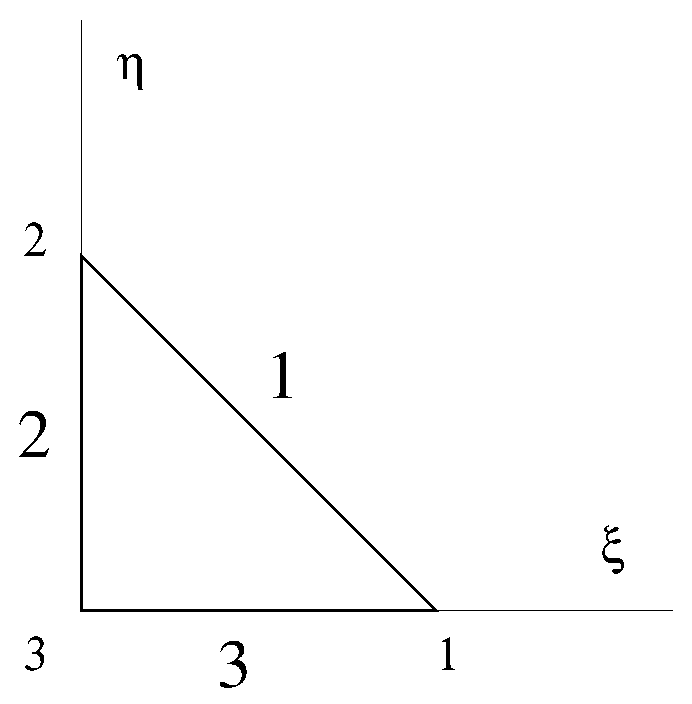
\includegraphics[width=60mm]{FIG/lintriangedges.eps}
\label{figlintriangedges}
\caption{Ordering of edges for triangular element with 3 nodes.}
\end{center}
\end{figure}

%%%%%%%%%%%%%%%%%%%%%%%%%%%%%%%%%%%%%%%%%%%%%%%%%%%%
\subsubsection{Triangular elements with six nodes}

\begin{table}[h]
\begin{center}
\begin{tabular}{|l|l|}
\hline
edge number & node numbers
\\ \hline
1 & 1, 2, 4
\\ \hline
2 & 2, 3, 5
\\ \hline
3 & 3, 1, 6
\\ \hline
\end{tabular}
\label{tabquadtriangedges}
\caption{Ordering of edges for triangular element with 6 nodes.}
\end{center}
\end{table}

\begin{figure}[h]
\begin{center}
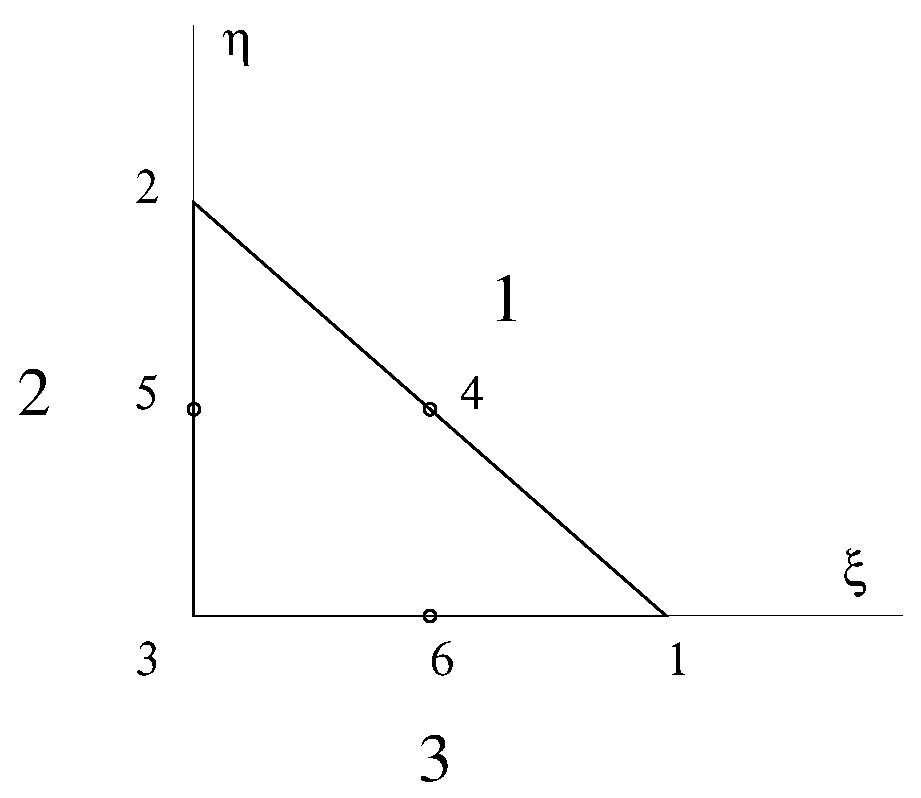
\includegraphics[width=80mm]{FIG/quadtriangedges.eps}
\label{figquadtriangedges}
\caption{Ordering of edges for triangular element with 6 nodes.}
\end{center}
\end{figure}

%%%%%%%%%%%%%%%%%%%%%%%%%%%%%%%%%%%%%%%%%%%%%
%%%%%%%%%%%%%%%%%%%%%%%%%%%%%%%%%%%%%%%%%%%%%
\subsection{Quadrilateral elements}

%%%%%%%%%%%%%%%%%%%%%%%%%%%%%%%%%%%%%%%%%%%%%
\subsubsection{Quadrilateral elements with four nodes}

\begin{table}[h]
\begin{center}
\begin{tabular}{|l|l|}
\hline
edge number & node numbers
\\ \hline
1 & 1, 2
\\ \hline
2 & 2, 3
\\ \hline
3 & 3, 4
\\ \hline
4 & 4, 1
\\ \hline
\end{tabular}
\label{tablinquadedges}
\caption{Ordering of edges for quadrilateral element with 4 nodes.}
\end{center}
\end{table}

\begin{figure}[h]
\begin{center}
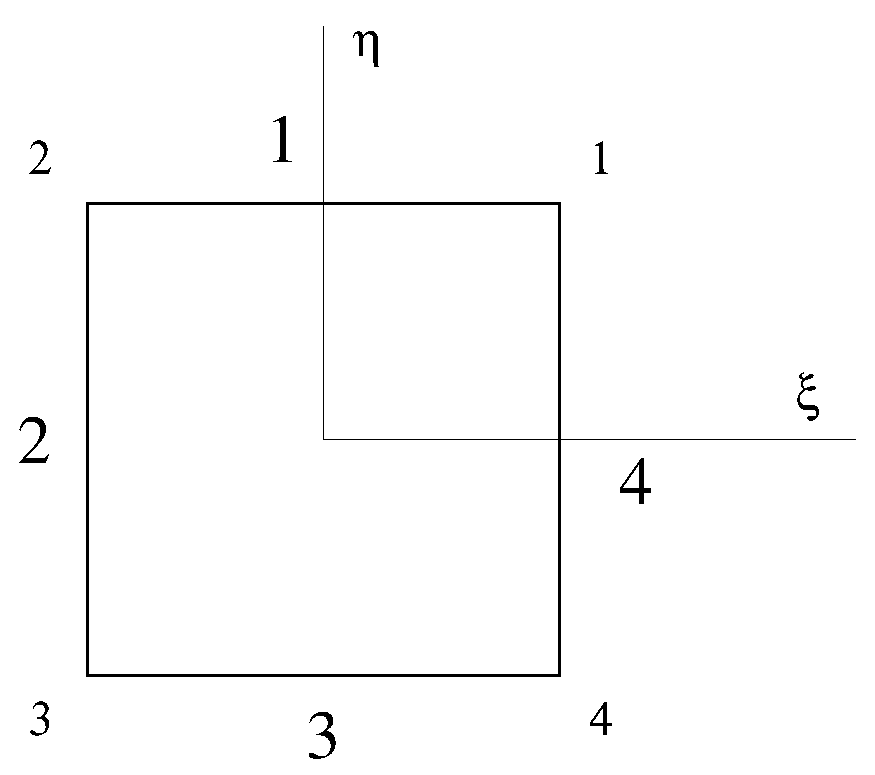
\includegraphics[width=60mm]{FIG/linquadedges.eps}
\label{figlinquadedges}
\caption{Ordering of edges for quadrilateral element with 4 nodes.}
\end{center}
\end{figure}

%%%%%%%%%%%%%%%%%%%%%%%%%%%%%%%%%%%%%%%%%%%%%
\subsubsection{Quadrilateral elements with eight nodes}

\begin{table}[h]
\begin{center}
\begin{tabular}{|l|l|}
\hline
edge number & node numbers
\\ \hline
1 & 1, 2, 5
\\ \hline
2 & 2, 3, 6
\\ \hline
3 & 3, 4, 7
\\ \hline
4 & 4, 1, 8
\\ \hline
\end{tabular}
\label{tabquadquadedges}
\caption{Ordering of edges for quadrilateral element with 8 nodes.}
\end{center}
\end{table}

\begin{figure}[h]
\begin{center}
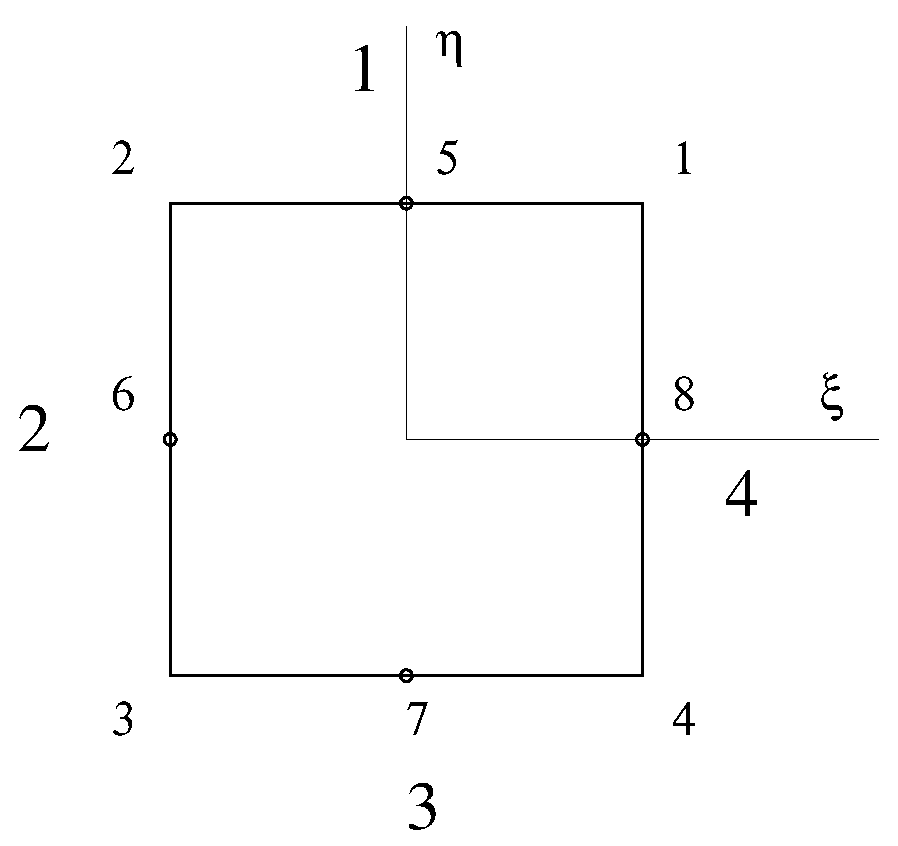
\includegraphics[width=60mm]{FIG/quadquadedges.eps}
\label{figquadquadedges}
\caption{Ordering of edges for quadrilateral element with 8 nodes.}
\end{center}
\end{figure}

%%%%%%%%%%%%%%%%%%%%%%%%%%%%%%%%%%%%%%%%%%%%%
%%%%%%%%%%%%%%%%%%%%%%%%%%%%%%%%%%%%%%%%%%%%%
\subsection{Hexahedral elements}

%%%%%%%%%%%%%%%%%%%%%%%%%%%%%%%%%%%%%%%%%%%%%
\subsubsection{Hexahedral elements with eight nodes}

\begin{table}[h]
\begin{center}
\begin{tabular}{|l|l|}
\hline
surface number & node numbers
\\ \hline
1 & 1, 4, 8, 5
\\ \hline
2 & 2, 1, 5, 6
\\ \hline
3 & 3, 2, 6, 7
\\ \hline
4 & 4, 3, 7, 8
\\ \hline
5 & 1, 2, 3, 4
\\ \hline
6 & 5, 6, 7, 8
\\ \hline
\end{tabular}
\label{tablinhexsurf}
\caption{Ordering of surfaces for hexahedral element with 8 nodes.}
\end{center}
\end{table}

\begin{figure}[h]
\begin{center}
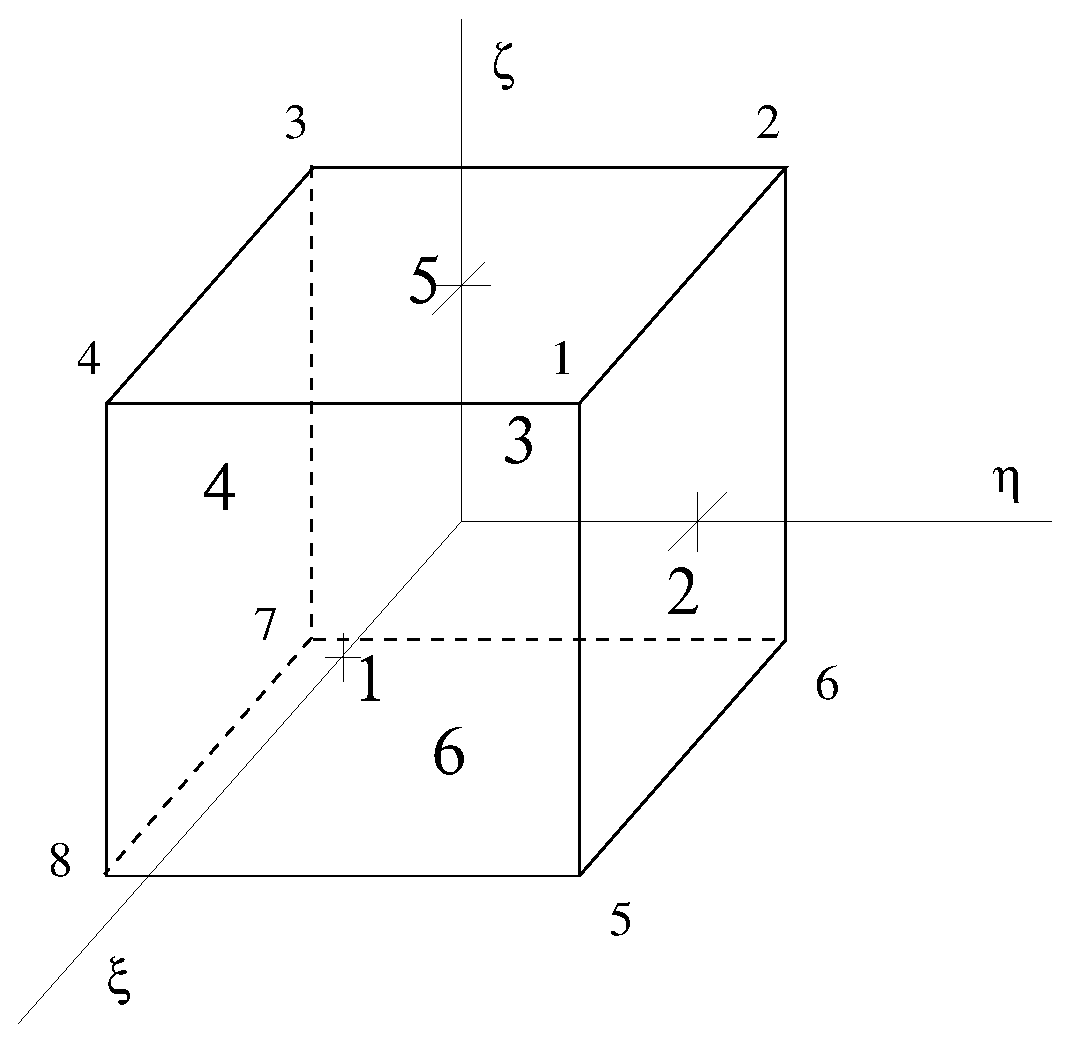
\includegraphics[width=60mm]{FIG/linhexsurf.eps}
\label{figlinhexsurf}
\caption{Ordering of surfaces for hexahedral element with 8 nodes.}
\end{center}
\end{figure}

%%%%%%%%%%%%%%%%%%%%%%%%%%%%%%%%%%%%%%%%%%%%%
\subsubsection{Hexahedral elements with twenty nodes}

\begin{table}[h]
\begin{center}
\begin{tabular}{|l|l|}
\hline
surface number & node numbers
\\ \hline
1 & 1, 4, 8, 5, 12, 16, 20, 13
\\ \hline
2 & 2, 1, 5, 6, 9, 13, 17, 14
\\ \hline
3 & 3, 2, 6, 7, 10, 14, 18, 15
\\ \hline
4 & 4, 3, 7, 8, 11, 15, 19, 16
\\ \hline
5 & 1, 2, 3, 4, 9, 10, 11, 12
\\ \hline
6 & 5, 6, 7, 8, 17, 18, 19, 20
\\ \hline
\end{tabular}
\label{tabquadhexsurf}
\caption{Ordering of surfaces for hexahedral element with 20 nodes.}
\end{center}
\end{table}

\begin{figure}[h]
\begin{center}
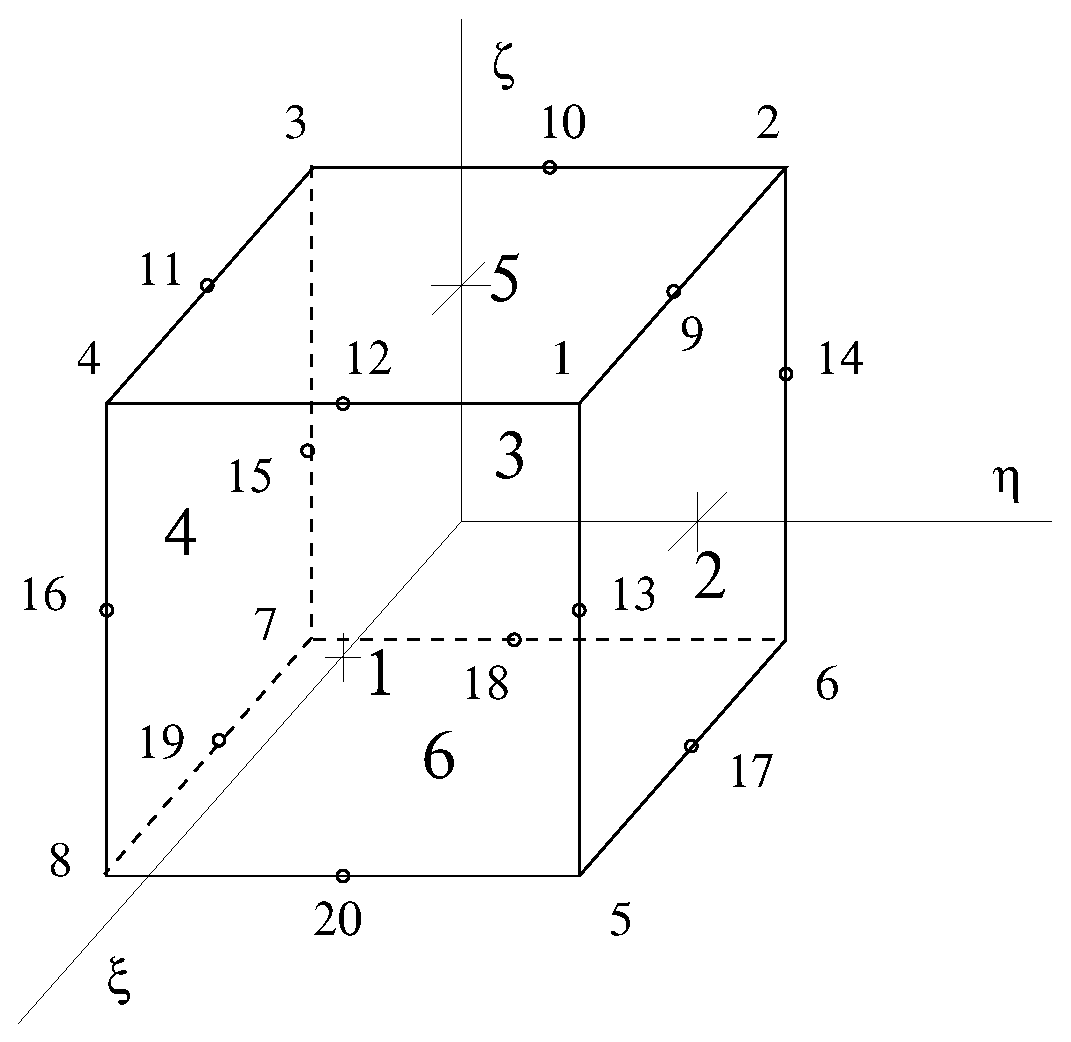
\includegraphics[width=60mm]{FIG/quadhexsurf.eps}
\label{figquadhexsurf}
\caption{Ordering of surfaces for hexahedral element with 20 nodes.}
\end{center}
\end{figure}

\chapter{Approximation functions}

%%%%%%%%%%%%%%%%%%%%%%%%%%%%%%%%%%%%%%%%%%%%%%%%%%%%%%%%%%%%%%%%%%%%%%%%%%%%%%%%%%%%%%%%%%%%%%%%
%%%%%%%%%%%%%%%%%%%%%%%%%%%%%%%%%%%%%%%%%%%%%%%%%%%%%%%%%%%%%%%%%%%%%%%%%%%%%%%%%%%%%%%%%%%%%%%%
%%%%%%%%%%%%%%%%%%%%%%%%%%%%%%%%%%%%%%%%%%%%%%%%%%%%%%%%%%%%%%%%%%%%%%%%%%%%%%%%%%%%%%%%%%%%%%%%
%%%%%%%%%%%%%%%%%%%%%%%%%%%%%%%%%%%%%%%%%%%%%%%%%%%%%%%%%%%%%%%%%%%%%%%%%%%%%%%%%%%%%%%%%%%%%%%%
%%%%%%%%%%%%%%%%%%%%%%%%%%%%%%%%%%%%%%%%%%%%%%%%%%%%%%%%%%%%%%%%%%%%%%%%%%%%%%%%%%%%%%%%%%%%%%%%
%%%%%%%%%%%%%%%%%%%%%%%%%%%%%%%%%%%%%%%%%%%%%%%%%%%%%%%%%%%%%%%%%%%%%%%%%%%%%%%%%%%%%%%%%%%%%%%%
%%%%%%%%%%%%%%%%%%%%%%%%%%%%%%%%%%%%%%%%%%%%%%%%%%%%%%%%%%%%%%%%%%%%%%%%%%%%%%%%%%%%%%%%%%%%%%%%
%%%%%%%%%%%%%%%%%%%%%%%%%%%%%%%%%%%%%%%%%%%%%%%%%%%%%%%%%%%%%%%%%%%%%%%%%%%%%%%%%%%%%%%%%%%%%%%%
\section{Linear approximation functions defined on triangles}
\begin{eqnarray}
\label{bflintrn1}
N_1^{(1)} &=& \xi\ ,
\\
\label{bflintrn2}
N_2^{(1)} &=& \eta\ ,
\\
\label{bflintrn3}
N_3^{(1)} &=& 1 - \xi - \eta\ .
\end{eqnarray}
\begin{figure}
\begin{center}
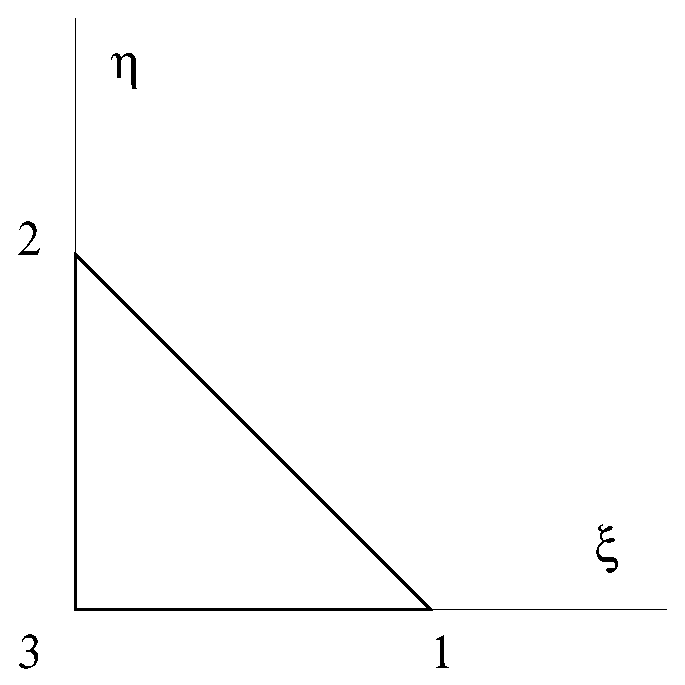
\includegraphics[width=80mm]{FIG/lintriang.eps}
\end{center}
\end{figure}
Partial derivatives with respect to $\xi$ have form
\begin{eqnarray}
\label{bflintrdx1}
\ppd{N_1^{(1)}}{\xi} &=& 1\ ,
\\
\label{bflintrdx2}
\ppd{N_2^{(1)}}{\xi} &=& 0\ ,
\\
\label{bflintrdx3}
\ppd{N_3^{(1)}}{\xi} &=& - 1\ .
\end{eqnarray}
Partial derivatives with respect to $\eta$ have form
\begin{eqnarray}
\label{bflintrdy1}
\ppd{N_1^{(1)}}{\eta} &=& 0\ ,
\\
\label{bflintrdy2}
\ppd{N_2^{(1)}}{\eta} &=& 1\ ,
\\
\label{bflintrdy3}
\ppd{N_3^{(1)}}{\eta} &=& - 1\ .
\end{eqnarray}


%%%%%%%%%%%%%%%%%%%%%%%%%%%%%%%%%%%%%%%%%%%%%%%%%%%%%%%%%%%%%%%%%%%%%%%%%%%%%%%%%%%%%%%%%%%%%%%%
%%%%%%%%%%%%%%%%%%%%%%%%%%%%%%%%%%%%%%%%%%%%%%%%%%%%%%%%%%%%%%%%%%%%%%%%%%%%%%%%%%%%%%%%%%%%%%%%
%%%%%%%%%%%%%%%%%%%%%%%%%%%%%%%%%%%%%%%%%%%%%%%%%%%%%%%%%%%%%%%%%%%%%%%%%%%%%%%%%%%%%%%%%%%%%%%%
%%%%%%%%%%%%%%%%%%%%%%%%%%%%%%%%%%%%%%%%%%%%%%%%%%%%%%%%%%%%%%%%%%%%%%%%%%%%%%%%%%%%%%%%%%%%%%%%
\section{Quadratic approximation functions defined on triangles}
\begin{eqnarray}
\label{bfquadtrn1}
N_1^{(2)} &=& 2\xi(\xi-0.5)\ ,
\\
\label{bfquadtrn2}
N_2^{(2)} &=& 2\eta(\eta-0.5)\ ,
\\
\label{bfquadtrn3}
N_3^{(2)} &=& 2(1 - \xi - \eta)(0.5-\xi-\eta)\ .
\\
\label{bfquadtrn4}
N_4^{(2)} &=& 4 \xi \eta \ ,
\\
\label{bfquadtrn5}
N_5^{(2)} &=& 4 \eta (1 - \xi - \eta)\ ,
\\
\label{bfquadtrn6}
N_6^{(2)} &=& 4 \xi (1 - \xi - \eta)\ ,
\\
\end{eqnarray}
\begin{figure}
\begin{center}
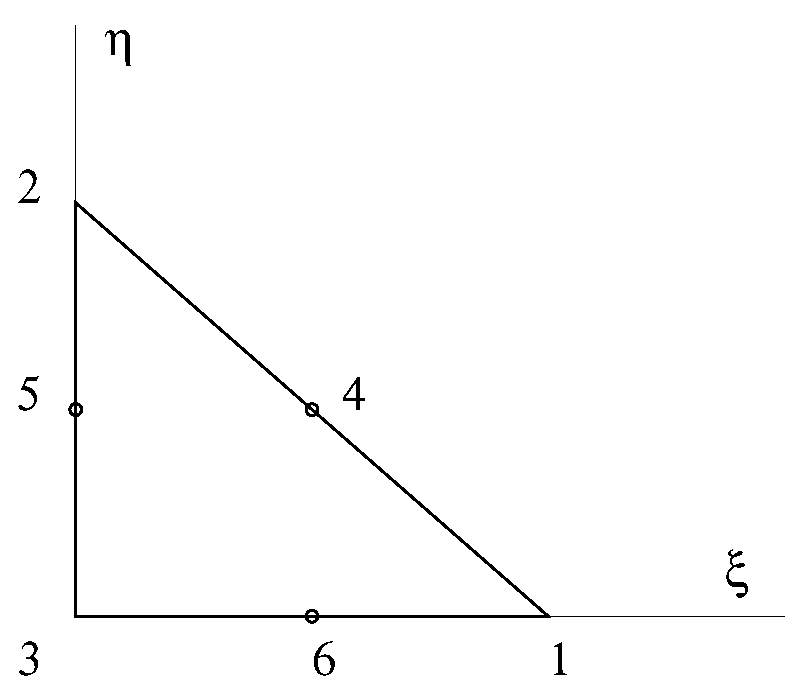
\includegraphics[width=80mm]{FIG/quadtriang.eps}
\end{center}
\end{figure}
Partial derivatives with respect to $\xi$ have form
\begin{eqnarray}
\label{bfquadtrdx1}
\ppd{N_1^{(2)}}{\xi} &=& 4 \xi - 1\ ,
\\
\label{bfquadtrdx2}
\ppd{N_2^{(2)}}{\xi} &=& 0\ ,
\\
\label{bfquadtrdx3}
\ppd{N_3^{(2)}}{\xi} &=& 4 \xi + 4 \eta - 3\ ,
\\
\label{bfquadtrdx4}
\ppd{N_4^{(2)}}{\xi} &=& 4 \eta\ ,
\\
\label{bfquadtrdx5}
\ppd{N_5^{(2)}}{\xi} &=& -4 \eta\ ,
\\
\label{bfquadtrdx6}
\ppd{N_6^{(2)}}{\xi} &=& 4 - 8 \xi - 4 \eta\ .
\end{eqnarray}
Partial derivatives with respect to $\eta$ have form
\begin{eqnarray}
\label{bfquadtrdy1}
\ppd{N_1^{(2)}}{\eta} &=& 0\ ,
\\
\label{bfquadtrdy2}
\ppd{N_2^{(2)}}{\eta} &=& 4 \eta -1\ ,
\\
\label{bfquadtrdy3}
\ppd{N_3^{(2)}}{\eta} &=& 4 \xi + 4 \eta -3\ ,
\\
\label{bfquadtrdy4}
\ppd{N_4^{(2)}}{\eta} &=& 4 \xi\ ,
\\
\label{bfquadtrdy5}
\ppd{N_5^{(2)}}{\eta} &=& 4 - 4 \xi - 8 \eta\ ,
\\
\label{bfquadtrdy6}
\ppd{N_6^{(2)}}{\eta} &=& - 4 \xi\ .
\end{eqnarray}



%%%%%%%%%%%%%%%%%%%%%%%%%%%%%%%%%%%%%%%%%%%%%%%%%%%%%%%%%%%%%%%%%%%%%%%%%%%%%%%%%%%%%%%%%%%%%%%%
%%%%%%%%%%%%%%%%%%%%%%%%%%%%%%%%%%%%%%%%%%%%%%%%%%%%%%%%%%%%%%%%%%%%%%%%%%%%%%%%%%%%%%%%%%%%%%%%
%%%%%%%%%%%%%%%%%%%%%%%%%%%%%%%%%%%%%%%%%%%%%%%%%%%%%%%%%%%%%%%%%%%%%%%%%%%%%%%%%%%%%%%%%%%%%%%%
%%%%%%%%%%%%%%%%%%%%%%%%%%%%%%%%%%%%%%%%%%%%%%%%%%%%%%%%%%%%%%%%%%%%%%%%%%%%%%%%%%%%%%%%%%%%%%%%
\section{Bi-linear approximation functions defined on quadrilateral elements}
$\xi$ and $\eta$ are natural coordinates defined on square $\langle-1;1\rangle\times\langle-1;1\rangle$. The functions
have form
\begin{eqnarray}
\label{bflinquadn1}
N_1^{(1)} &=& \del{1}{4} (1 + \xi) (1 + \eta)\ ,
\\
\label{bflinquadn2}
N_2^{(1)} &=& \del{1}{4} (1 - \xi) (1 + \eta)\ ,
\\
\label{bflinquadn3}
N_3^{(1)} &=& \del{1}{4} (1 - \xi) (1 - \eta)\ ,
\\
\label{bflinquadn4}
N_4^{(1)} &=& \del{1}{4} (1 + \xi) (1 - \eta)\ .
\end{eqnarray}
\begin{figure}
\begin{center}
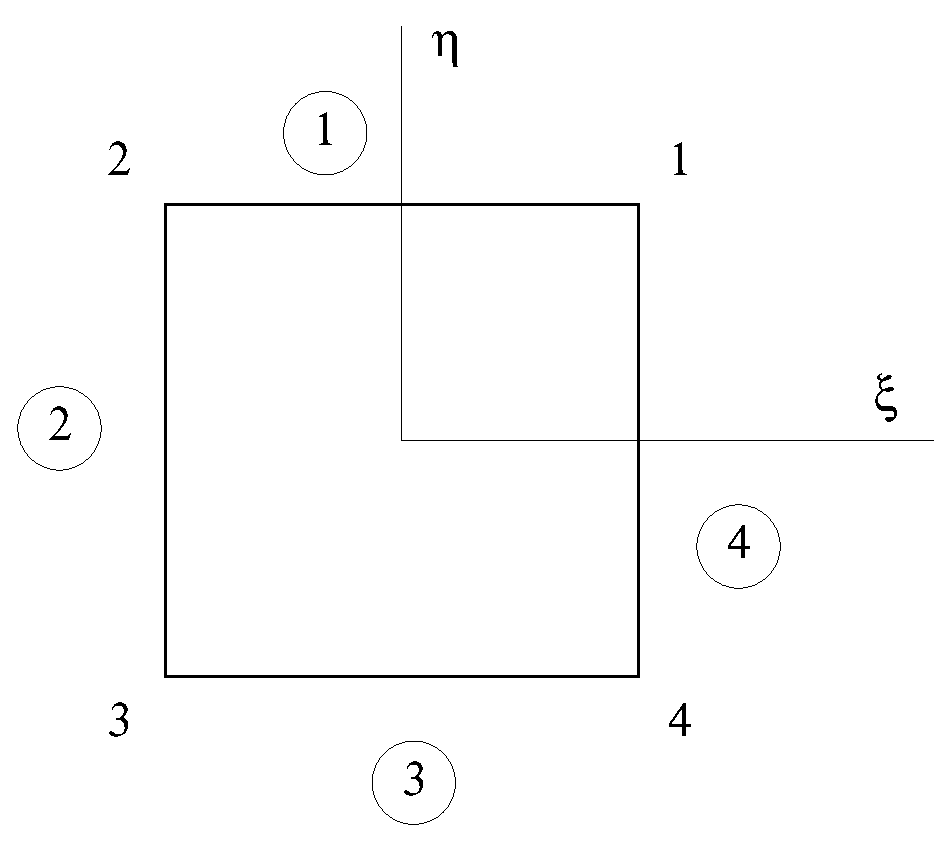
\includegraphics[width=80mm]{FIG/linquad.eps}
\end{center}
\end{figure}
Partial derivatives with respect to $\xi$ have form
\begin{eqnarray}
\label{bflinquaddx1}
\ppd{N_1^{(1)}}{\xi} &=& \del{1}{4} (1 + \eta)\ ,
\\
\label{bflinquaddx2}
\ppd{N_2^{(1)}}{\xi} &=& - \del{1}{4} (1 + \eta)\ ,
\\
\label{bflinquaddx3}
\ppd{N_3^{(1)}}{\xi} &=& - \del{1}{4} (1 - \eta)\ ,
\\
\label{bflinquaddx4}
\ppd{N_4^{(1)}}{\xi} &=& \del{1}{4} (1 - \eta)\ .
\end{eqnarray}
Partial derivatives with respect to $\eta$ have form
\begin{eqnarray}
\label{bflinquaddy1}
\ppd{N_1^{(1)}}{\eta} &=& \del{1}{4} (1 + \xi)\ ,
\\
\label{bflinquaddy2}
\ppd{N_2^{(1)}}{\eta} &=& \del{1}{4} (1 - \xi)\ ,
\\
\label{bflinquaddy3}
\ppd{N_3^{(1)}}{\eta} &=& - \del{1}{4} (1 - \xi)\ ,
\\
\label{bflinquaddy4}
\ppd{N_4^{(1)}}{\eta} &=& - \del{1}{4} (1 + \xi)\ .
\end{eqnarray}

%%%%%%%%%%%%%%%%%%%%%%%%%%%%%%%%%%%%%%%%%%%%%%%%%%%%%%%%%%%%%%%%%%%%%%%%%%%%%%%%%%%%%%%%%%%%%%%%
%%%%%%%%%%%%%%%%%%%%%%%%%%%%%%%%%%%%%%%%%%%%%%%%%%%%%%%%%%%%%%%%%%%%%%%%%%%%%%%%%%%%%%%%%%%%%%%%
%%%%%%%%%%%%%%%%%%%%%%%%%%%%%%%%%%%%%%%%%%%%%%%%%%%%%%%%%%%%%%%%%%%%%%%%%%%%%%%%%%%%%%%%%%%%%%%%
%%%%%%%%%%%%%%%%%%%%%%%%%%%%%%%%%%%%%%%%%%%%%%%%%%%%%%%%%%%%%%%%%%%%%%%%%%%%%%%%%%%%%%%%%%%%%%%%
\section{Bi-quadratic approximation functions defined on quadrilateral elements}
$\xi$ and $\eta$ are natural coordinates defined on square $\langle-1;1\rangle\times\langle-1;1\rangle$. The functions
have form
\begin{eqnarray}
\label{bfquadquadn1}
N_1^{(2)} &=& \del{1}{4} (1 + \xi) (1 + \eta) (\xi + \eta - 1)\ ,
\\
\label{bfquadquadn2}
N_2^{(2)} &=& \del{1}{4} (1 - \xi) (1 + \eta) (- \xi + \eta - 1)\ ,
\\
\label{bfquadquadn3}
N_3^{(2)} &=& \del{1}{4} (1 - \xi) (1 - \eta) (- \xi - \eta - 1)\ ,
\\
\label{bfquadquadn4}
N_4^{(2)} &=& \del{1}{4} (1 + \xi) (1 - \eta) (\xi - \eta - 1)\ ,
\\
\label{bfquadquadn5}
N_5^{(2)} &=& \del{1}{2} (1 - \xi^2) (1 + \eta)\ ,
\\
\label{bfquadquadn6}
N_6^{(2)} &=& \del{1}{2} (1 - \xi) (1 - \eta^2)\ ,
\\
\label{bfquadquadn7}
N_7^{(2)} &=& \del{1}{2} (1 - \xi^2) (1 - \eta)\ ,
\\
\label{bfquadquadn8}
N_8^{(2)} &=& \del{1}{2} (1 + \xi) (1 - \eta^2)\ .
\end{eqnarray}
\begin{figure}
\begin{center}
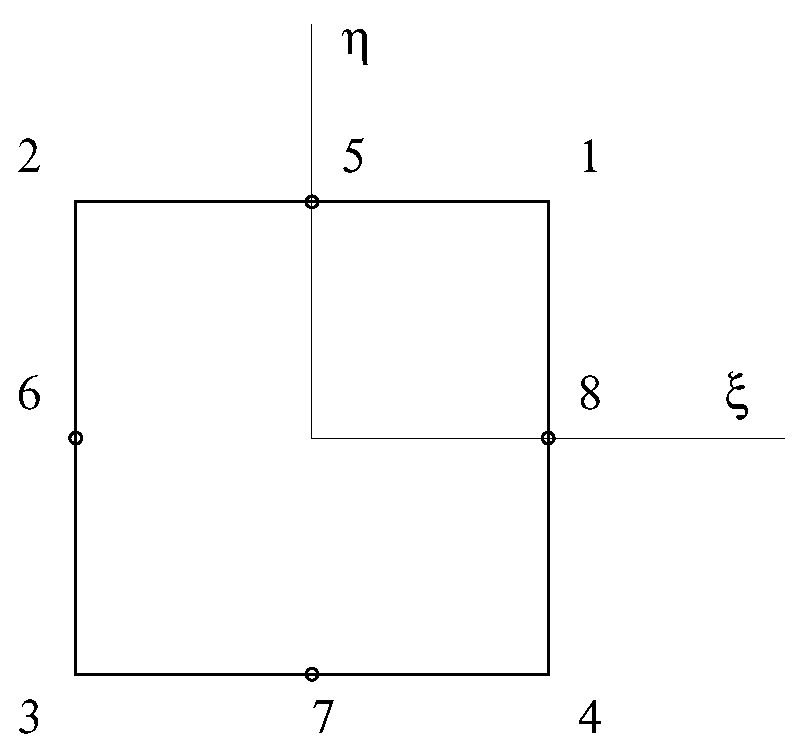
\includegraphics[width=80mm]{FIG/quadquad.eps}
\end{center}
\end{figure}
Partial derivatives with respect to $\xi$ have form
\begin{eqnarray}
\label{bfquadquaddx1}
\ppd{N_1^{(2)}}{\xi} &=& \del{1}{4} (1 + \eta) (\xi + \eta - 1) +
\del{1}{4} (1 + \xi) (1 + \eta)\ ,
\\
\label{bfquadquaddx2}
\ppd{N_2^{(2)}}{\xi} &=& - \del{1}{4} (1 + \eta) (- \xi + \eta - 1) -
\del{1}{4} (1 - \xi) (1 + \eta)\ ,
\\
\label{bfquadquaddx3}
\ppd{N_3^{(2)}}{\xi} &=& - \del{1}{4} (1 - \eta) (- \xi - \eta - 1) -
\del{1}{4} (1 - \xi) (1 - \eta)\ ,
\\
\label{bfquadquaddx4}
\ppd{N_4^{(2)}}{\xi} &=& \del{1}{4} (1 - \eta) (\xi - \eta - 1) +
\del{1}{4} (1 + \xi) (1 - \eta)\ ,
\\
\label{bfquadquaddx5}
\ppd{N_5^{(2)}}{\xi} &=& - \xi (1 + \eta)\ ,
\\
\label{bfquadquaddx6}
\ppd{N_6^{(2)}}{\xi} &=& - \del{1}{2} (1 - \eta^2)\ ,
\\
\label{bfquadquaddx7}
\ppd{N_7^{(2)}}{\xi} &=& - \xi (1 - \eta)\ ,
\\
\label{bfquadquaddx8}
\ppd{N_8^{(2)}}{\xi} &=& \del{1}{2} (1 - \eta^2)\ .
\end{eqnarray}
Partial derivatives with respect to $\eta$ have form
\begin{eqnarray}
\label{bfquadquaddy1}
\ppd{N_1^{(2)}}{\eta} &=& \del{1}{4} (1 + \xi) (\xi + \eta - 1) +
\del{1}{4} (1 + \xi) (1 + \eta)\ ,
\\
\label{bfquadquaddy2}
\ppd{N_2^{(2)}}{\eta} &=& \del{1}{4} (1 - \xi) (- \xi + \eta - 1) +
\del{1}{4} (1 - \xi) (1 + \eta)\ ,
\\
\label{bfquadquaddy3}
\ppd{N_3^{(2)}}{\eta} &=& - \del{1}{4} (1 - \xi) (- \xi - \eta - 1) -
\del{1}{4} (1 - \xi) (1 - \eta)\ ,
\\
\label{bfquadquaddy4}
\ppd{N_4^{(2)}}{\eta} &=& - \del{1}{4} (1 + \xi) (\xi - \eta - 1) -
\del{1}{4} (1 + \xi) (1 - \eta)\ ,
\\
\label{bfquadquaddy5}
\ppd{N_5^{(2)}}{\eta} &=& \del{1}{2} (1 - \xi^2)\ ,
\\
\label{bfquadquaddy6}
\ppd{N_6^{(2)}}{\eta} &=& (1 - \xi) (- \eta)\ ,
\\
\label{bfquadquaddy7}
\ppd{N_7^{(2)}}{\eta} &=& - \del{1}{2} (1 - \xi^2)\ ,
\\
\label{bfquadquaddy8}
\ppd{N_8^{(2)}}{\eta} &=& (1 + \xi) (- \eta)\ .
\end{eqnarray}

%%%%%%%%%%%%%%%%%%%%%%%%%%%%%%%%%%%%%%%%%%%%%%%%%%%%%%%%%%%%%%%%%%%%%%%%%%%%%
%%%%%%%%%%%%%%%%%%%%%%%%%%%%%%%%%%%%%%%%%%%%%%%%%%%%%%%%%%%%%%%%%%%%%%%%%%%%%%%%%%%%%%%%%%%%%%%%
%%%%%%%%%%%%%%%%%%%%%%%%%%%%%%%%%%%%%%%%%%%%%%%%%%%%%%%%%%%%%%%%%%%%%%%%%%%%%%%%%%%%%%%%%%%%%%%%
%%%%%%%%%%%%%%%%%%%%%%%%%%%%%%%%%%%%%%%%%%%%%%%%%%%%%%%%%%%%%%%%%%%%%%%%%%%%%%%%%%%%%%%%%%%%%%%%
%%%%%%%%%%%%%%%%%%%%%%%%%%%%%%%%%%%%%%%%%%%%%%%%%%%%%%%%%%%%%%%%%%%%%%%%%%%%%%%%%%%%%%%%%%%%%%%%
\section{Tri-linear approximation functions defined on hexahedral elements}
$\xi$, $\eta$ and $\zeta$ are natural coordinates defined on cube
$\langle-1;1\rangle\times\langle-1;1\rangle\times\langle-1;1\rangle$. The functions have form
\begin{eqnarray}
\label{bflinhexn1}
N_1^{(1)} &=& \del{1}{8} (1 + \xi) (1 + \eta) (1 + \zeta)\ ,
\\
\label{bflinhexn2}
N_2^{(1)} &=& \del{1}{8} (1 - \xi) (1 + \eta) (1 + \zeta)\ ,
\\
\label{bflinhexn3}
N_3^{(1)} &=& \del{1}{8} (1 - \xi) (1 - \eta) (1 + \zeta)\ ,
\\
\label{bflinhexn4}
N_4^{(1)} &=& \del{1}{8} (1 + \xi) (1 - \eta) (1 + \zeta)\ ,
\\
\label{bflinhexn5}
N_5^{(1)} &=& \del{1}{8} (1 + \xi) (1 + \eta) (1 - \zeta)\ ,
\\
\label{bflinhexn6}
N_6^{(1)} &=& \del{1}{8} (1 - \xi) (1 + \eta) (1 - \zeta)\ ,
\\
\label{bflinhexn7}
N_7^{(1)} &=& \del{1}{8} (1 - \xi) (1 - \eta) (1 - \zeta)\ ,
\\
\label{bflinhexn8}
N_8^{(1)} &=& \del{1}{8} (1 + \xi) (1 - \eta) (1 - \zeta)\ .
\end{eqnarray}
\begin{figure}
\begin{center}
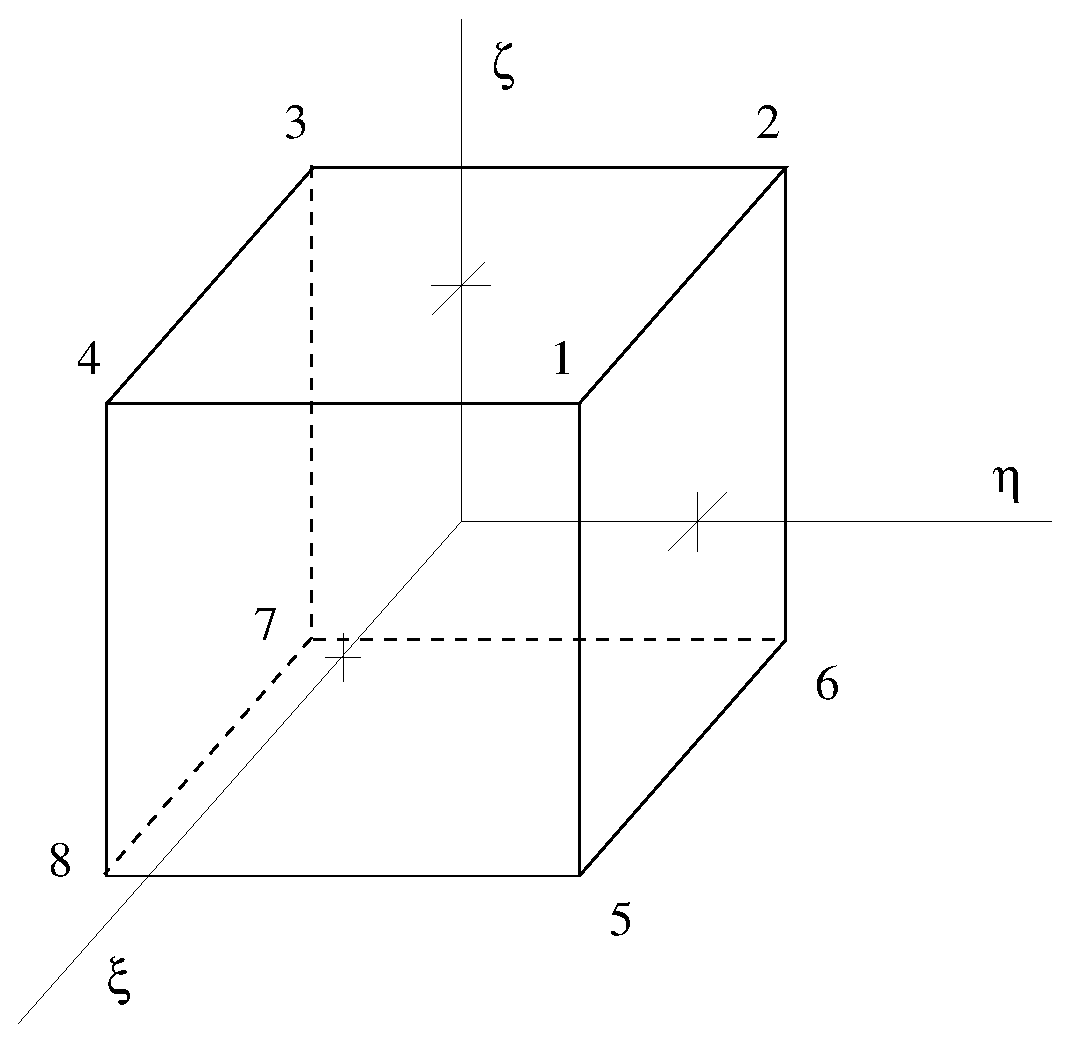
\includegraphics[width=80mm]{FIG/linhex.eps}
\end{center}
\end{figure}
Partial derivatives with respect to $\xi$ have form
\begin{eqnarray}
\label{bflinhexdx1}
\ppd{N_1^{(1)}}{\xi} &=& \del{1}{8} (1 + \eta) (1 + \zeta)\ ,
\\
\label{bflinhexdx2}
\ppd{N_2^{(1)}}{\xi} &=& - \del{1}{8} (1 + \eta) (1 + \zeta)\ ,
\\
\label{bflinhexdx3}
\ppd{N_3^{(1)}}{\xi} &=& - \del{1}{8} (1 - \eta) (1 + \zeta)\ ,
\\
\label{bflinhexdx4}
\ppd{N_4^{(1)}}{\xi} &=& \del{1}{8} (1 - \eta) (1 + \zeta)\ ,
\\
\label{bflinhexdx5}
\ppd{N_5^{(1)}}{\xi} &=& \del{1}{8} (1 + \eta) (1 - \zeta)\ ,
\\
\label{bflinhexdx6}
\ppd{N_6^{(1)}}{\xi} &=& - \del{1}{8} (1 + \eta) (1 - \zeta)\ ,
\\
\label{bflinhexdx7}
\ppd{N_7^{(1)}}{\xi} &=& - \del{1}{8} (1 - \eta) (1 - \zeta)\ ,
\\
\label{bflinhexdx8}
\ppd{N_8^{(1)}}{\xi} &=& \del{1}{8} (1 - \eta) (1 - \zeta)\ .
\end{eqnarray}
Partial derivatives with respect to $\eta$ have form
\begin{eqnarray}
\label{bflinhexdy1}
\ppd{N_1^{(1)}}{\eta} &=& \del{1}{8} (1 + \xi) (1 + \zeta)\ ,
\\
\label{bflinhexdy2}
\ppd{N_2^{(1)}}{\eta} &=& \del{1}{8} (1 - \xi) (1 + \zeta)\ ,
\\
\label{bflinhexdy3}
\ppd{N_3^{(1)}}{\eta} &=& - \del{1}{8} (1 - \xi) (1 + \zeta)\ ,
\\
\label{bflinhexdy4}
\ppd{N_4^{(1)}}{\eta} &=& - \del{1}{8} (1 + \xi) (1 + \zeta)\ ,
\\
\label{bflinhexdy5}
\ppd{N_5^{(1)}}{\eta} &=& \del{1}{8} (1 + \xi) (1 - \zeta)\ ,
\\
\label{bflinhexdy6}
\ppd{N_6^{(1)}}{\eta} &=& \del{1}{8} (1 - \xi) (1 - \zeta)\ ,
\\
\label{bflinhexdy7}
\ppd{N_7^{(1)}}{\eta} &=& - \del{1}{8} (1 - \xi) (1 - \zeta)\ ,
\\
\label{bflinhexdy8}
\ppd{N_8^{(1)}}{\eta} &=& - \del{1}{8} (1 + \xi) (1 - \zeta)\ .
\end{eqnarray}
Partial derivatives with respect to $\zeta$ have form
\begin{eqnarray}
\label{bflinhexdz1}
\ppd{N_1^{(1)}}{\zeta} &=& \del{1}{8} (1 + \xi) (1 + \eta)\ ,
\\
\label{bflinhexdz2}
\ppd{N_2^{(1)}}{\zeta} &=& \del{1}{8} (1 - \xi) (1 + \eta)\ ,
\\
\label{bflinhexdz3}
\ppd{N_3^{(1)}}{\zeta} &=& \del{1}{8} (1 - \xi) (1 - \eta)\ ,
\\
\label{bflinhexdz4}
\ppd{N_4^{(1)}}{\zeta} &=& \del{1}{8} (1 + \xi) (1 - \eta)\ ,
\\
\label{bflinhexdz5}
\ppd{N_5^{(1)}}{\zeta} &=& - \del{1}{8} (1 + \xi) (1 + \eta)\ ,
\\
\label{bflinhexdz6}
\ppd{N_6^{(1)}}{\zeta} &=& - \del{1}{8} (1 - \xi) (1 + \eta)\ ,
\\
\label{bflinhexdz7}
\ppd{N_7^{(1)}}{\zeta} &=& - \del{1}{8} (1 - \xi) (1 - \eta)\ ,
\\
\label{bflinhexdz8}
\ppd{N_8^{(1)}}{\zeta} &=& - \del{1}{8} (1 + \xi) (1 - \eta)\ .
\end{eqnarray}



%%%%%%%%%%%%%%%%%%%%%%%%%%%%%%%%%%%%%%%%%%%%%%%%%%%%%%%%%%%%%%%%%%%%%%%%%%%%%%%%%%%%%%%%%%%%%%%%
%%%%%%%%%%%%%%%%%%%%%%%%%%%%%%%%%%%%%%%%%%%%%%%%%%%%%%%%%%%%%%%%%%%%%%%%%%%%%%%%%%%%%%%%%%%%%%%%
%%%%%%%%%%%%%%%%%%%%%%%%%%%%%%%%%%%%%%%%%%%%%%%%%%%%%%%%%%%%%%%%%%%%%%%%%%%%%%%%%%%%%%%%%%%%%%%%
%%%%%%%%%%%%%%%%%%%%%%%%%%%%%%%%%%%%%%%%%%%%%%%%%%%%%%%%%%%%%%%%%%%%%%%%%%%%%%%%%%%%%%%%%%%%%%%%
\section{Tri-quadratic approximation functions defined on hexahedral elements}
$\xi$, $\eta$ and $\zeta$ are natural coordinates defined on cube
$\langle-1;1\rangle\times\langle-1;1\rangle\times\langle-1;1\rangle$. The functions have form
\begin{eqnarray}
\label{bfquadhexn1}
N_{1}^{(2)} &=& \del{1}{8} (1 + \xi) (1 + \eta) (1 + \zeta)
(\xi + \eta + \zeta - 2)\ ,
\\ \label{bfquadhexn2}
N_{2}^{(2)} &=& \del{1}{8} (1 - \xi) (1 + \eta) (1 + \zeta)
(- \xi + \eta + \zeta - 2)\ ,
\\ \label{bfquadhexn3}
N_{3}^{(2)} &=& \del{1}{8} (1 - \xi) (1 - \eta) (1 + \zeta)
(- \xi - \eta + \zeta - 2)\ ,
\\ \label{bfquadhexn4}
N_{4}^{(2)} &=& \del{1}{8} (1 + \xi) (1 - \eta) (1 + \zeta)
(\xi - \eta + \zeta - 2)\ ,
\\ \label{bfquadhexn5}
N_{5}^{(2)} &=& \del{1}{8} (1 + \xi) (1 + \eta) (1 - \zeta)
(\xi + \eta - \zeta - 2)\ ,
\\ \label{bfquadhexn6}
N_{6}^{(2)} &=& \del{1}{8} (1 - \xi) (1 + \eta) (1 - \zeta)
(- \xi + \eta - \zeta - 2)\ ,
\\ \label{bfquadhexn7}
N_{7}^{(2)} &=& \del{1}{8} (1 - \xi) (1 - \eta) (1 - \zeta)
(- \xi - \eta - \zeta - 2)\ ,
\\ \label{bfquadhexn8}
N_{8}^{(2)} &=& \del{1}{8} (1 + \xi) (1 - \eta) (1 - \zeta)
(\xi - \eta - \zeta - 2)\ ,
\\ \label{bfquadhexn9}
N_{9}^{(2)} &=& \del{1}{4} (1 - \xi^2) (1 + \eta) (1 + \zeta)\ ,
\\ \label{bfquadhexn10}
N_{10}^{(2)} &=& \del{1}{4} (1 - \xi) (1 - \eta^2) (1 + \zeta)\ ,
\\ \label{bfquadhexn11}
N_{11}^{(2)} &=& \del{1}{4} (1 - \xi^2) (1 - \eta) (1 + \zeta)\ ,
\\ \label{bfquadhexn12}
N_{12}^{(2)} &=& \del{1}{4} (1 + \xi) (1 - \eta^2) (1 + \zeta)\ ,
\\ \label{bfquadhexn13}
N_{13}^{(2)} &=& \del{1}{4} (1 + \xi) (1 + \eta) (1 - \zeta^2)\ ,
\\ \label{bfquadhexn14}
N_{14}^{(2)} &=& \del{1}{4} (1 - \xi) (1 + \eta) (1 - \zeta^2)\ ,
\\ \label{bfquadhexn15}
N_{15}^{(2)} &=& \del{1}{4} (1 - \xi) (1 - \eta) (1 - \zeta^2)\ ,
\\ \label{bfquadhexn16}
N_{16}^{(2)} &=& \del{1}{4} (1 + \xi) (1 - \eta) (1 - \zeta^2)\ ,
\\ \label{bfquadhexn17}
N_{17}^{(2)} &=& \del{1}{4} (1 - \xi^2) (1 + \eta) (1 - \zeta)\ ,
\\ \label{bfquadhexn18}
N_{18}^{(2)} &=& \del{1}{4} (1 - \xi) (1 - \eta^2) (1 - \zeta)\ ,
\\ \label{bfquadhexn19}
N_{19}^{(2)} &=& \del{1}{4} (1 - \xi^2) (1 - \eta) (1 - \zeta)\ ,
\\ \label{bfquadhexn20}
N_{20}^{(2)} &=& \del{1}{4} (1 + \xi) (1 - \eta^2) (1 - \zeta)\ .
\end{eqnarray}
\begin{figure}
\begin{center}
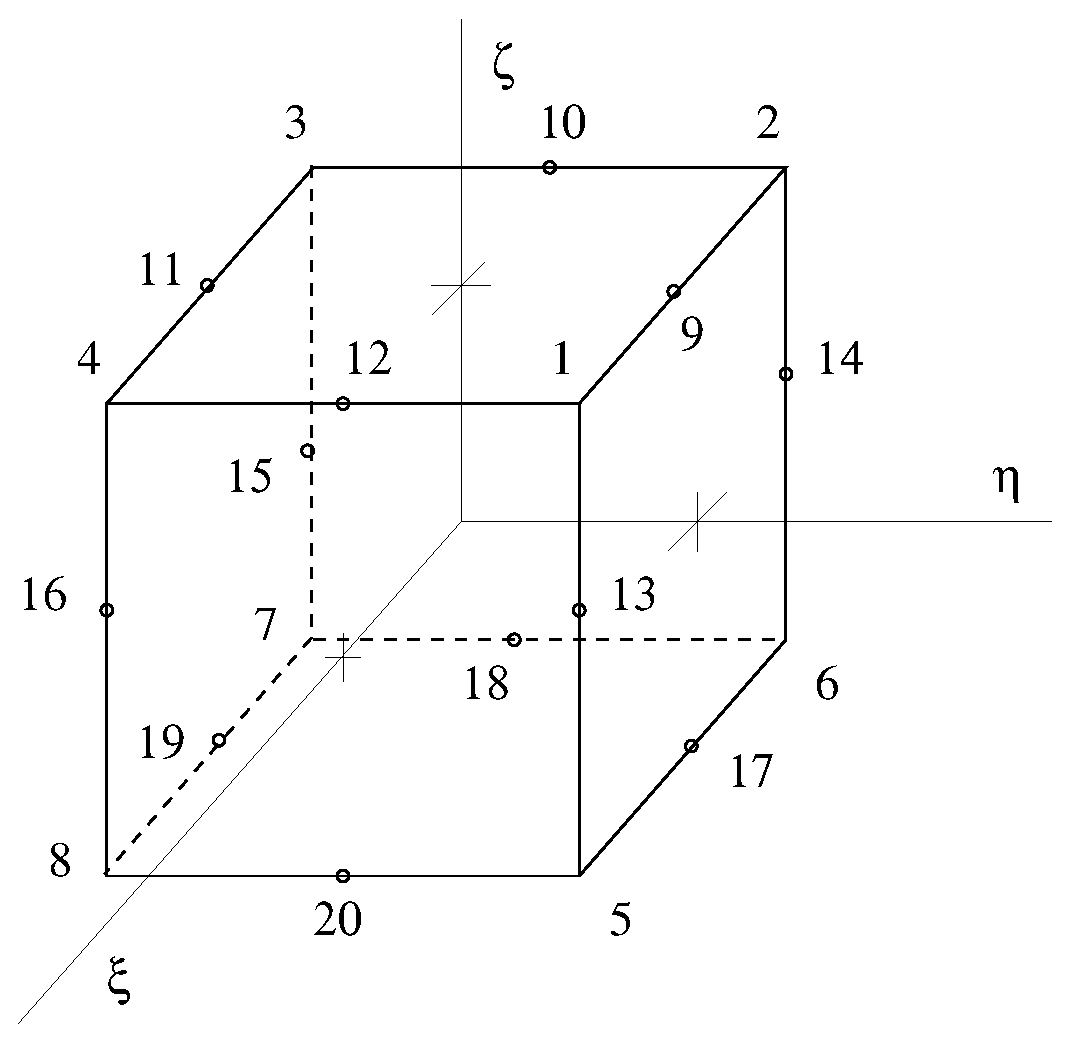
\includegraphics[width=80mm]{FIG/quadhex.eps}
\end{center}
\end{figure}
Partial derivatives with respect to $\xi$ have form
\begin{eqnarray}
\label{bfquadhexdx1}
\ppd{N_{1}^{(2)}}{\xi} &=& \del{1}{8} (1 + \eta) (1 + \zeta)
(\xi + \eta + \zeta - 2) + \del{1}{8} (1 + \xi) (1 + \eta) (1 + \zeta)\ ,
\\ \label{bfquadhexdx2}
\ppd{N_{2}^{(2)}}{\xi} &=& - \del{1}{8} (1 + \eta) (1 + \zeta)
(- \xi + \eta + \zeta - 2) - \del{1}{8} (1 - \xi) (1 + \eta) (1 + \zeta)\ ,
\\ \label{bfquadhexdx3}
\ppd{N_{3}^{(2)}}{\xi} &=& - \del{1}{8} (1 - \eta) (1 + \zeta)
(- \xi - \eta + \zeta - 2) - \del{1}{8} (1 - \xi) (1 - \eta) (1 + \zeta)\ ,
\\ \label{bfquadhexdx4}
\ppd{N_{4}^{(2)}}{\xi} &=& \del{1}{8} (1 - \eta) (1 + \zeta)
(\xi - \eta + \zeta - 2) + \del{1}{8} (1 + \xi) (1 - \eta) (1 + \zeta)\ ,
\\ \label{bfquadhexdx5}
\ppd{N_{5}^{(2)}}{\xi} &=& \del{1}{8} (1 + \eta) (1 - \zeta)
(\xi + \eta - \zeta - 2) + \del{1}{8} (1 + \xi) (1 + \eta) (1 - \zeta)\ ,
\\ \label{bfquadhexdx6}
\ppd{N_{6}^{(2)}}{\xi} &=& - \del{1}{8} (1 + \eta) (1 - \zeta)
(- \xi + \eta - \zeta - 2) - \del{1}{8} (1 - \xi) (1 + \eta) (1 - \zeta)\ ,
\\ \label{bfquadhexdx7}
\ppd{N_{7}^{(2)}}{\xi} &=& - \del{1}{8} (1 - \eta) (1 - \zeta)
(- \xi - \eta - \zeta - 2) - \del{1}{8} (1 - \xi) (1 - \eta) (1 - \zeta)\ ,
\\ \label{bfquadhexdx8}
\ppd{N_{8}^{(2)}}{\xi} &=& \del{1}{8} (1 - \eta) (1 - \zeta)
(\xi - \eta - \zeta - 2) + \del{1}{8} (1 + \xi) (1 - \eta) (1 - \zeta)\ ,
\\ \label{bfquadhexdx9}
\ppd{N_{9}^{(2)}}{\xi} &=& - \del{1}{2} \xi (1 + \eta) (1 + \zeta)\ ,
\\ \label{bfquadhexdx10}
\ppd{N_{10}^{(2)}}{\xi} &=& - \del{1}{4} (1 - \eta^2) (1 + \zeta)\ ,
\\ \label{bfquadhexdx11}
\ppd{N_{11}^{(2)}}{\xi} &=& - \del{1}{2} \xi (1 - \eta) (1 + \zeta)\ ,
\\ \label{bfquadhexdx12}
\ppd{N_{12}^{(2)}}{\xi} &=& \del{1}{4} (1 - \eta^2) (1 + \zeta)\ ,
\\ \label{bfquadhexdx13}
\ppd{N_{13}^{(2)}}{\xi} &=& \del{1}{4} (1 + \eta) (1 - \zeta^2)\ ,
\\ \label{bfquadhexdx14}
\ppd{N_{14}^{(2)}}{\xi} &=& - \del{1}{4} (1 + \eta) (1 - \zeta^2)\ ,
\\ \label{bfquadhexdx15}
\ppd{N_{15}^{(2)}}{\xi} &=& - \del{1}{4} (1 - \eta) (1 - \zeta^2)\ ,
\\ \label{bfquadhexdx16}
\ppd{N_{16}^{(2)}}{\xi} &=& \del{1}{4} (1 - \eta) (1 - \zeta^2)\ ,
\\ \label{bfquadhexdx17}
\ppd{N_{17}^{(2)}}{\xi} &=& - \del{1}{2} \xi (1 + \eta) (1 - \zeta)\ ,
\\ \label{bfquadhexdx18}
\ppd{N_{18}^{(2)}}{\xi} &=& - \del{1}{4} (1 - \eta^2) (1 - \zeta)\ ,
\\ \label{bfquadhexdx19}
\ppd{N_{19}^{(2)}}{\xi} &=& - \del{1}{2} \xi (1 - \eta) (1 - \zeta)\ ,
\\ \label{bfquadhexdx20}
\ppd{N_{20}^{(2)}}{\xi} &=& \del{1}{4} (1 - \eta^2) (1 - \zeta)\ .
\end{eqnarray}
Partial derivatives with respect to $\eta$ have form
\begin{eqnarray}
\label{bfquadhexdy1}
\ppd{N_{1}^{(2)}}{\eta} &=& \del{1}{8} (1 + \xi) (1 + \zeta)
(\xi + \eta + \zeta - 2) + \del{1}{8} (1 + \xi) (1 + \eta) (1 + \zeta)\ ,
\\ \label{bfquadhexdy2}
\ppd{N_{2}^{(2)}}{\eta} &=& \del{1}{8} (1 - \xi) (1 + \zeta)
(- \xi + \eta + \zeta - 2) + \del{1}{8} (1 - \xi) (1 + \eta) (1 + \zeta)\ ,
\\ \label{bfquadhexdy3}
\ppd{N_{3}^{(2)}}{\eta} &=& - \del{1}{8} (1 - \xi) (1 + \zeta)
(- \xi - \eta + \zeta - 2) - \del{1}{8} (1 - \xi) (1 - \eta) (1 + \zeta)\ ,
\\ \label{bfquadhexdy4}
\ppd{N_{4}^{(2)}}{\eta} &=& - \del{1}{8} (1 + \xi) (1 + \zeta)
(\xi - \eta + \zeta - 2) - \del{1}{8} (1 + \xi) (1 - \eta) (1 + \zeta)\ ,
\\ \label{bfquadhexdy5}
\ppd{N_{5}^{(2)}}{\eta} &=& \del{1}{8} (1 + \xi) (1 - \zeta)
(\xi + \eta - \zeta - 2) + \del{1}{8} (1 + \xi) (1 + \eta) (1 - \zeta)\ ,
\\ \label{bfquadhexdy6}
\ppd{N_{6}^{(2)}}{\eta} &=& \del{1}{8} (1 - \xi) (1 - \zeta)
(- \xi + \eta - \zeta - 2) + \del{1}{8} (1 - \xi) (1 + \eta) (1 - \zeta)\ ,
\\ \label{bfquadhexdy7}
\ppd{N_{7}^{(2)}}{\eta} &=& - \del{1}{8} (1 - \xi) (1 - \zeta)
(- \xi - \eta - \zeta - 2) - \del{1}{8} (1 - \xi) (1 - \eta) (1 - \zeta)\ ,
\\ \label{bfquadhexdy8}
\ppd{N_{8}^{(2)}}{\eta} &=& - \del{1}{8} (1 + \xi) (1 - \zeta)
(\xi - \eta - \zeta - 2) - \del{1}{8} (1 + \xi) (1 - \eta) (1 - \zeta)\ ,
\\ \label{bfquadhexdy9}
\ppd{N_{9}^{(2)}}{\eta} &=& \del{1}{4} (1 - \xi^2) (1 + \zeta)\ ,
\\ \label{bfquadhexdy10}
\ppd{N_{10}^{(2)}}{\eta} &=& - \del{1}{2} (1 - \xi) \eta (1 + \zeta)\ ,
\\ \label{bfquadhexdy11}
\ppd{N_{11}^{(2)}}{\eta} &=& - \del{1}{4} (1 - \xi^2) (1 + \zeta)\ ,
\\ \label{bfquadhexdy12}
\ppd{N_{12}^{(2)}}{\eta} &=& - \del{1}{2} (1 + \xi) \eta (1 + \zeta)\ ,
\\ \label{bfquadhexdy13}
\ppd{N_{13}^{(2)}}{\eta} &=& \del{1}{4} (1 + \xi) (1 - \zeta^2)\ ,
\\ \label{bfquadhexdy14}
\ppd{N_{14}^{(2)}}{\eta} &=& \del{1}{4} (1 - \xi) (1 - \zeta^2)\ ,
\\ \label{bfquadhexdy15}
\ppd{N_{15}^{(2)}}{\eta} &=& - \del{1}{4} (1 - \xi) (1 - \zeta^2)\ ,
\\ \label{bfquadhexdy16}
\ppd{N_{16}^{(2)}}{\eta} &=& - \del{1}{4} (1 + \xi) (1 - \zeta^2)\ ,
\\ \label{bfquadhexdy17}
\ppd{N_{17}^{(2)}}{\eta} &=& \del{1}{4} (1 - \xi^2) (1 - \zeta)\ ,
\\ \label{bfquadhexdy18}
\ppd{N_{18}^{(2)}}{\eta} &=& - \del{1}{2} (1 - \xi) \eta (1 - \zeta)\ ,
\\ \label{bfquadhexdy19}
\ppd{N_{19}^{(2)}}{\eta} &=& - \del{1}{4} (1 - \xi^2) (1 - \zeta)\ ,
\\ \label{bfquadhexdy20}
\ppd{N_{20}^{(2)}}{\eta} &=& - \del{1}{2} (1 + \xi) \eta (1 - \zeta)\ .
\end{eqnarray}
Partial derivatives with respect to $\zeta$ have form
\begin{eqnarray}
\label{bfquadhexdz1}
\ppd{N_{1}^{(2)}}{\zeta} &=& \del{1}{8} (1 + \xi) (1 + \eta)
(\xi + \eta + \zeta - 2) + \del{1}{8} (1 + \xi) (1 + \eta) (1 + \zeta)\ ,
\\ \label{bfquadhexdz2}
\ppd{N_{2}^{(2)}}{\zeta} &=& \del{1}{8} (1 - \xi) (1 + \eta)
(- \xi + \eta + \zeta - 2) + \del{1}{8} (1 - \xi) (1 + \eta) (1 + \zeta)\ ,
\\ \label{bfquadhexdz3}
\ppd{N_{3}^{(2)}}{\zeta} &=& \del{1}{8} (1 - \xi) (1 - \eta)
(- \xi - \eta + \zeta - 2) + \del{1}{8} (1 - \xi) (1 - \eta) (1 + \zeta)\ ,
\\ \label{bfquadhexdz4}
\ppd{N_{4}^{(2)}}{\zeta} &=& \del{1}{8} (1 + \xi) (1 - \eta)
(\xi - \eta + \zeta - 2) + \del{1}{8} (1 + \xi) (1 - \eta) (1 + \zeta)\ ,
\\ \label{bfquadhexdz5}
\ppd{N_{5}^{(2)}}{\zeta} &=& - \del{1}{8} (1 + \xi) (1 + \eta)
(\xi + \eta - \zeta - 2) - \del{1}{8} (1 + \xi) (1 + \eta) (1 - \zeta)\ ,
\\ \label{bfquadhexdz6}
\ppd{N_{6}^{(2)}}{\zeta} &=& - \del{1}{8} (1 - \xi) (1 + \eta)
(- \xi + \eta - \zeta - 2) - \del{1}{8} (1 - \xi) (1 + \eta) (1 - \zeta)\ ,
\\ \label{bfquadhexdz7}
\ppd{N_{7}^{(2)}}{\zeta} &=& - \del{1}{8} (1 - \xi) (1 - \eta)
(- \xi - \eta - \zeta - 2) - \del{1}{8} (1 - \xi) (1 - \eta) (1 - \zeta)\ ,
\\ \label{bfquadhexdz8}
\ppd{N_{8}^{(2)}}{\zeta} &=& - \del{1}{8} (1 + \xi) (1 - \eta)
(\xi - \eta - \zeta - 2) - \del{1}{8} (1 + \xi) (1 - \eta) (1 - \zeta)\ ,
\\ \label{bfquadhexdz9}
\ppd{N_{9}^{(2)}}{\zeta} &=& \del{1}{4} (1 - \xi^2) (1 + \eta)\ ,
\\ \label{bfquadhexdz10}
\ppd{N_{10}^{(2)}}{\zeta} &=& \del{1}{4} (1 - \xi) (1 - \eta^2)\ ,
\\ \label{bfquadhexdz11}
\ppd{N_{11}^{(2)}}{\zeta} &=& \del{1}{4} (1 - \xi^2) (1 - \eta)\ ,
\\ \label{bfquadhexdz12}
\ppd{N_{12}^{(2)}}{\zeta} &=& \del{1}{4} (1 + \xi) (1 - \eta^2)\ ,
\\ \label{bfquadhexdz13}
\ppd{N_{13}^{(2)}}{\zeta} &=& - \del{1}{2} (1 + \xi) (1 + \eta) \zeta\ ,
\\ \label{bfquadhexdz14}
\ppd{N_{14}^{(2)}}{\zeta} &=& - \del{1}{2} (1 - \xi) (1 + \eta) \zeta\ ,
\\ \label{bfquadhexdz15}
\ppd{N_{15}^{(2)}}{\zeta} &=& - \del{1}{2} (1 - \xi) (1 - \eta) \zeta\ ,
\\ \label{bfquadhexdz16}
\ppd{N_{16}^{(2)}}{\zeta} &=& - \del{1}{2} (1 + \xi) (1 - \eta) \zeta\ ,
\\ \label{bfquadhexdz17}
\ppd{N_{17}^{(2)}}{\zeta} &=& - \del{1}{4} (1 - \xi^2) (1 + \eta)\ ,
\\ \label{bfquadhexdz18}
\ppd{N_{18}^{(2)}}{\zeta} &=& - \del{1}{4} (1 - \xi) (1 - \eta^2)\ ,
\\ \label{bfquadhexdz19}
\ppd{N_{19}^{(2)}}{\zeta} &=& - \del{1}{4} (1 - \xi^2) (1 - \eta)\ ,
\\ \label{bfquadhexdz20}
\ppd{N_{20}^{(2)}}{\zeta} &=& - \del{1}{4} (1 + \xi) (1 - \eta^2)\ .
\end{eqnarray}

%%%%%%%%%%%%%%%%%%%%%%%%%%%%%%%%%%%%%%%%%%%%%%%%%%%%%%%%%%%%%%%%%%%%
%%%%%%%%%%%%%%%%%%%%%%%%%%%%%%%%%%%%%%%%%%%%%%%%%%%%%%%%%%%%%%%%%%%%

%%%%%%%%%%%%%%%%%%%%%%%%%%%%%%%%%%%%%%%%%%%%%%%%%%%%%%%%%%%%%%%%%%%%%%%%%%%%%
%%%%%%%%%%%%%%%%%%%%%%%%%%%%%%%%%%%%%%%%%%%%%%%%%%%%%%%%%%%%%%%%%%%%%%%%%%%%%%%%%%%%%%%%%%%%%%%%
%%%%%%%%%%%%%%%%%%%%%%%%%%%%%%%%%%%%%%%%%%%%%%%%%%%%%%%%%%%%%%%%%%%%%%%%%%%%%%%%%%%%%%%%%%%%%%%%
%%%%%%%%%%%%%%%%%%%%%%%%%%%%%%%%%%%%%%%%%%%%%%%%%%%%%%%%%%%%%%%%%%%%%%%%%%%%%%%%%%%%%%%%%%%%%%%%
%%%%%%%%%%%%%%%%%%%%%%%%%%%%%%%%%%%%%%%%%%%%%%%%%%%%%%%%%%%%%%%%%%%%%%%%%%%%%%%%%%%%%%%%%%%%%%%%
\section{Linear approximation functions defined on wedge elements}
$\xi$, $\eta$ and $\zeta$ are natural coordinates. The functions have form
\begin{eqnarray}
\label{bflinwedn1}
N_1^{(1)} &=& \del{1}{2} \xi (1 + \zeta)\ ,
\\ \label{bflinwedn2}
N_2^{(1)} &=& \del{1}{2} \eta (1 + \zeta)\ ,
\\ \label{bflinwedn3}
N_3^{(1)} &=& \del{1}{2} (1 - \xi -\eta) (1 + \zeta)\ ,
\\ \label{bflinwedn4}
N_4^{(1)} &=& \del{1}{2} \xi (1 - \zeta)\ ,
\\ \label{bflinwedn5}
N_5^{(1)} &=& \del{1}{2} \eta (1 - \zeta)\ ,
\\ \label{bflinwedn6}
N_6^{(1)} &=& \del{1}{2} (1 - \xi -\eta) (1 - \zeta)\ ,
\end{eqnarray}
\begin{figure}
\begin{center}
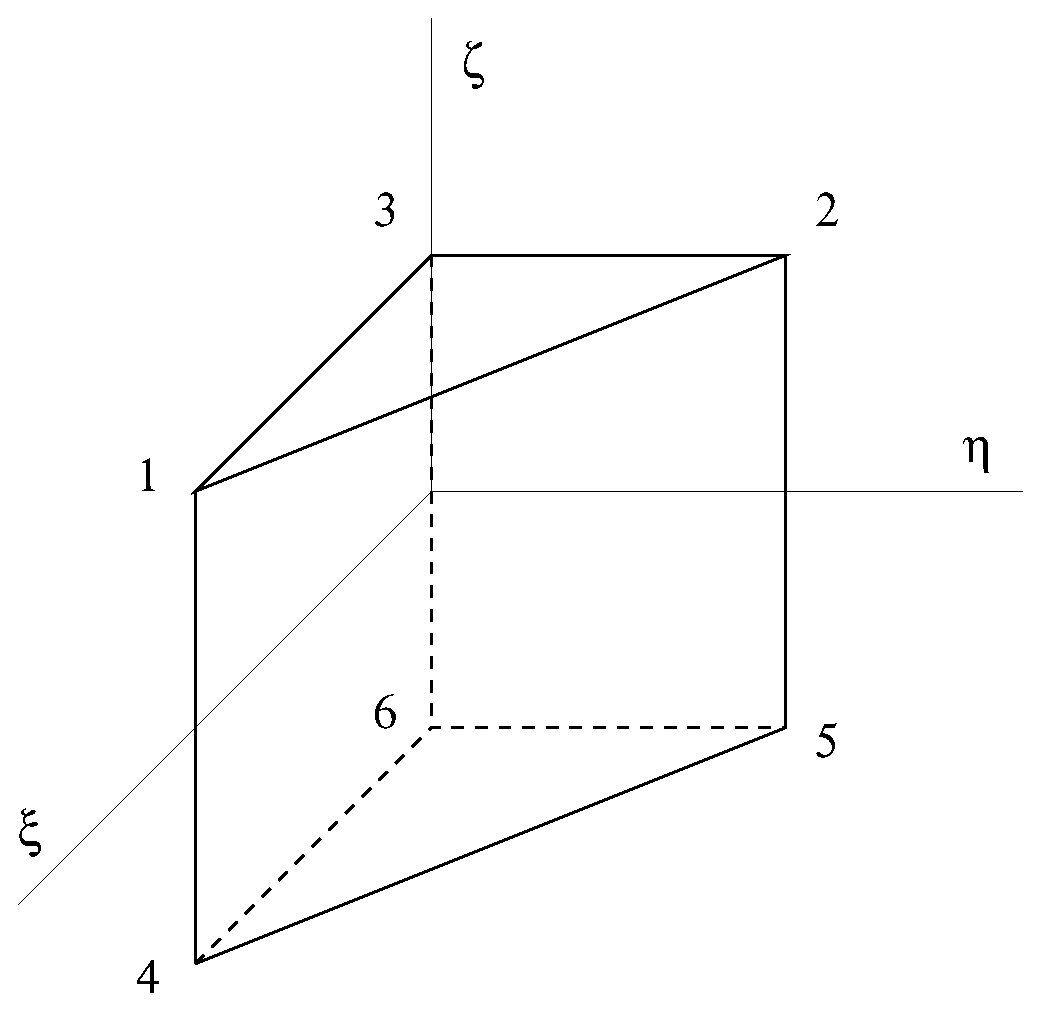
\includegraphics[width=80mm]{FIG/linwedge.eps}
\end{center}
\end{figure}
Partial derivatives with respect to $\xi$ have form
\begin{eqnarray}
\label{bflinweddx1}
\ppd{N_1^{(1)}}{\xi} &=& \del{1}{2} (1 + \zeta)\ ,
\\ \label{bflinweddx2}
\ppd{N_2^{(1)}}{\xi} &=& 0\ ,
\\ \label{bflinweddx3}
\ppd{N_3^{(1)}}{\xi} &=& - \del{1}{2} (1 + \zeta)\ ,
\\ \label{bflinweddx4}
\ppd{N_4^{(1)}}{\xi} &=& \del{1}{2} (1 - \zeta)\ ,
\\ \label{bflinweddx5}
\ppd{N_5^{(1)}}{\xi} &=& 0\ ,
\\ \label{bflinweddx6}
\ppd{N_6^{(1)}}{\xi} &=& - \del{1}{2} (1 - \zeta)\ ,
\end{eqnarray}
Partial derivatives with respect to $\eta$ have form
\begin{eqnarray}
\label{bflinweddy1}
\ppd{N_1^{(1)}}{\eta} &=& 0\ ,
\\ \label{bflinweddy2}
\ppd{N_2^{(1)}}{\eta} &=& \del{1}{2} (1 + \zeta)\ ,
\\ \label{bflinweddy3}
\ppd{N_3^{(1)}}{\eta} &=& - \del{1}{2} (1 + \zeta)\ ,
\\ \label{bflinweddy4}
\ppd{N_4^{(1)}}{\eta} &=& 0\ ,
\\ \label{bflinweddy5}
\ppd{N_5^{(1)}}{\eta} &=& \del{1}{2} (1 - \zeta)\ ,
\\ \label{bflinweddy6}
\ppd{N_6^{(1)}}{\eta} &=& - \del{1}{2} (1 - \zeta)\ ,
\end{eqnarray}
Partial derivatives with respect to $\zeta$ have form
\begin{eqnarray}
\label{bflinweddz1}
\ppd{N_1^{(1)}}{\zeta} &=& \del{\xi}{2}\ ,
\\ \label{bflinweddz2}
\ppd{N_2^{(1)}}{\zeta} &=& \del{\eta}{2}\ ,
\\ \label{bflinweddz3}
\ppd{N_3^{(1)}}{\zeta} &=& \del{1}{2} (1 - \xi - \eta)\ ,
\\ \label{bflinweddz4}
\ppd{N_4^{(1)}}{\zeta} &=& - \del{\xi}{2}\ ,
\\ \label{bflinweddz5}
\ppd{N_5^{(1)}}{\zeta} &=& - \del{\eta}{2}\ ,
\\ \label{bflinweddz6}
\ppd{N_6^{(1)}}{\zeta} &=& - \del{1}{2} (1 - \xi - \eta)\ ,
\end{eqnarray}

%%%%%%%%%%%%%%%%%%%%%%%%%%%%%%%%%%%%%%%%%%%%%%%%%%%%%%%%%%%%%%%%%%%%%%%%%%%%%
%%%%%%%%%%%%%%%%%%%%%%%%%%%%%%%%%%%%%%%%%%%%%%%%%%%%%%%%%%%%%%%%%%%%%%%%%%%%%%%%%%%%%%%%%%%%%%%%
%%%%%%%%%%%%%%%%%%%%%%%%%%%%%%%%%%%%%%%%%%%%%%%%%%%%%%%%%%%%%%%%%%%%%%%%%%%%%%%%%%%%%%%%%%%%%%%%
%%%%%%%%%%%%%%%%%%%%%%%%%%%%%%%%%%%%%%%%%%%%%%%%%%%%%%%%%%%%%%%%%%%%%%%%%%%%%%%%%%%%%%%%%%%%%%%%
%%%%%%%%%%%%%%%%%%%%%%%%%%%%%%%%%%%%%%%%%%%%%%%%%%%%%%%%%%%%%%%%%%%%%%%%%%%%%%%%%%%%%%%%%%%%%%%%
\section{Quadratic approximation functions defined on wedge elements}
$\xi$, $\eta$ and $\zeta$ are natural coordinates. The functions have form
\begin{eqnarray}
\label{bfquadwedn1}
N_1^{(2)} &=& \xi(\xi-0.5)(1 + \zeta)\zeta\ ,
\\
\label{bfquadwedn2}
N_2^{(2)} &=& \eta(\eta-0.5)(1 + \zeta)\zeta\ ,
\\
\label{bfquadwedn3}
N_3^{(2)} &=& (1 - \xi - \eta)(0.5-\xi-\eta)(1 + \zeta)\zeta\ .
\\
\label{bfquadwedn4}
N_4^{(2)} &=& \xi(\xi-0.5)(\zeta - 1)\zeta\ ,
\\
\label{bfquadwedn5}
N_5^{(2)} &=& \eta(\eta-0.5)(\zeta - 1)\zeta\ ,
\\
\label{bfquadwedn6}
N_6^{(2)} &=& (1 - \xi - \eta)(0.5-\xi-\eta)(\zeta - 1)\zeta\ .
\\
\label{bfquadwedn7}
N_7^{(2)} &=& 2 \xi \eta (1 + \zeta)\ ,
\\
\label{bfquadwedn8}
N_8^{(2)} &=& 2 \eta (1 - \xi - \eta)(1 + \zeta)\ ,
\\
\label{bfquadwedn9}
N_9^{(2)} &=& 2 \xi (1 - \xi - \eta)(1 + \zeta)\ ,
\\
\label{bfquadwedn10}
N_{10}^{(2)} &=& \xi (1 - \zeta^2)\ ,
\\
\label{bfquadwedn11}
N_{11}^{(2)} &=& \eta (1 - \zeta^2)\ ,
\\
\label{bfquadwedn12}
N_{12}^{(2)} &=& (1 - \xi - \eta)(1 - \zeta^2)\ ,
\\
\label{bfquadwedn13}
N_{13}^{(2)} &=& 2 \xi \eta (1 - \zeta)\ ,
\\
\label{bfquadwedn14}
N_{14}^{(2)} &=& 2 \eta (1 - \xi - \eta)(1 - \zeta)\ ,
\\
\label{bfquadwedn15}
N_{15}^{(2)} &=& 2 \xi (1 - \xi - \eta)(1 - \zeta)\ ,
\end{eqnarray}


\begin{figure}
\begin{center}
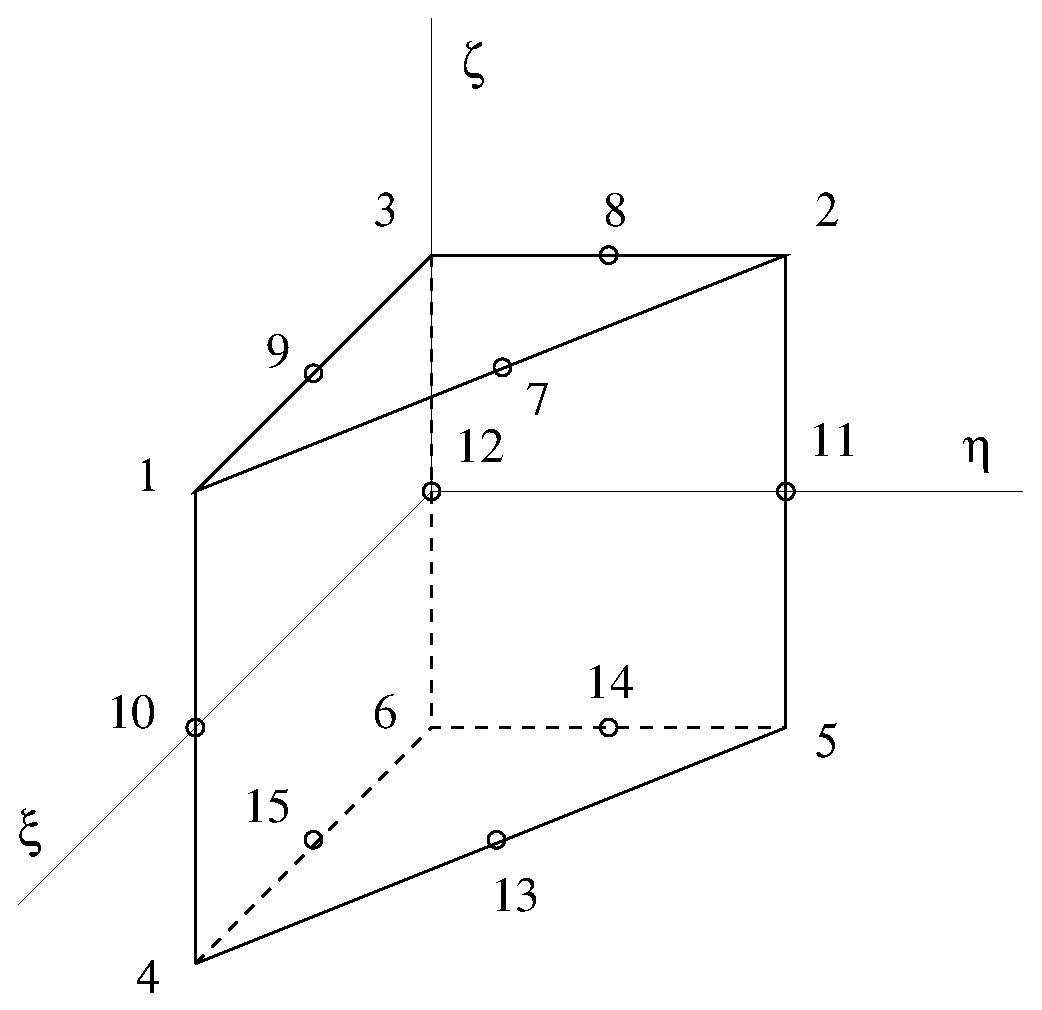
\includegraphics[width=80mm]{FIG/quadwedge.eps}
\end{center}
\end{figure}

Partial derivatives with respect to $\xi$ have form
\begin{eqnarray}
\label{bfquadweddx1}
\ppd{N_1^{(2)}}{\xi} &=& (2 \xi - 0.5) (1 + \zeta)\zeta\ ,
\\
\label{bfquadweddx2}
\ppd{N_2^{(2)}}{\xi} &=& 0\ ,
\\
\label{bfquadweddx3}
\ppd{N_3^{(2)}}{\xi} &=& (2\xi + 2\eta - \del{3}{2})(1 + \zeta)\zeta\ .
\\
\label{bfquadweddx4}
\ppd{N_4^{(2)}}{\xi} &=& (2\xi-0.5)(\zeta - 1)\zeta\ ,
\\
\label{bfquadweddx5}
\ppd{N_5^{(2)}}{\xi} &=& 0\ ,
\\
\label{bfquadweddx6}
\ppd{N_6^{(2)}}{\xi} &=& (2 \xi + 2\eta -\del{3}{2})(\zeta-1)\zeta\ .
\\
\label{bfquadweddx7}
\ppd{N_7^{(2)}}{\xi} &=& 2 \eta (1 + \zeta)\ ,
\\
\label{bfquadweddx8}
\ppd{N_8^{(2)}}{\xi} &=& - 2 \eta (1 + \zeta)\ ,
\\
\label{bfquadweddx9}
\ppd{N_9^{(2)}}{\xi} &=& (2 - 4\xi - 2\eta)(1 + \zeta)\ ,
\\
\label{bfquadweddx10}
\ppd{N_{10}^{(2)}}{\xi} &=& (1 - \zeta^2)\ ,
\\
\label{bfquadweddx11}
\ppd{N_{11}^{(2)}}{\xi} &=& 0\ ,
\\
\label{bfquadweddx12}
\ppd{N_{12}^{(2)}}{\xi} &=& \zeta^2 - 1\ ,
\\
\label{bfquadweddx13}
\ppd{N_{13}^{(2)}}{\xi} &=& 2 \eta (1 - \zeta)\ ,
\\
\label{bfquadweddx14}
\ppd{N_{14}^{(2)}}{\xi} &=& 2 \eta (\zeta - 1)\ ,
\\
\label{bfquadweddx15}
\ppd{N_{15}^{(2)}}{\xi} &=& (2 - 4\xi - 2\eta)(1 - \zeta)\ .
\end{eqnarray}



Partial derivatives with respect to $\eta$ have form
\begin{eqnarray}
\label{bfquadweddy1}
\ppd{N_1^{(2)}}{\eta} &=& 0\ ,
\\
\label{bfquadweddy2}
\ppd{N_2^{(2)}}{\eta} &=& (2\eta-0.5)(1 + \zeta)\zeta\ ,
\\
\label{bfquadweddy3}
\ppd{N_3^{(2)}}{\eta} &=& (2\xi + 2\eta -\del{3}{2})(1 + \zeta)\zeta\ ,
\\
\label{bfquadweddy4}
\ppd{N_4^{(2)}}{\eta} &=& 0\ ,
\\
\label{bfquadweddy5}
\ppd{N_5^{(2)}}{\eta} &=& (2\eta-0.5)(\zeta - 1)\zeta\ ,
\\
\label{bfquadweddy6}
\ppd{N_6^{(2)}}{\eta} &=& (2\xi + 2\eta - \del{3}{2})(\zeta - 1)\zeta\ .
\\
\label{bfquadweddy7}
\ppd{N_7^{(2)}}{\eta} &=& 2 \xi (1 + \zeta)\ ,
\\
\label{bfquadweddy8}
\ppd{N_8^{(2)}}{\eta} &=& (2 - 2\xi - 4\eta)(1 + \zeta)\ ,
\\
\label{bfquadweddy9}
\ppd{N_9^{(2)}}{\eta} &=& -2 \xi (1 + \zeta)\ ,
\\
\label{bfquadweddy10}
\ppd{N_{10}^{(2)}}{\eta} &=& 0\ ,
\\
\label{bfquadweddy11}
\ppd{N_{11}^{(2)}}{\eta} &=& 1 - \zeta^2\ ,
\\
\label{bfquadweddy12}
\ppd{N_{12}^{(2)}}{\eta} &=& \zeta^2 - 1\ ,
\\
\label{bfquadweddy13}
\ppd{N_{13}^{(2)}}{\eta} &=& 2 \xi (1 - \zeta)\ ,
\\
\label{bfquadweddy14}
\ppd{N_{14}^{(2)}}{\eta} &=& (2 - 2\xi - 4\eta)(1 - \zeta)\ ,
\\
\label{bfquadweddy15}
\ppd{N_{15}^{(2)}}{\eta} &=& 2 \xi (\zeta - 1)\ ,
\end{eqnarray}


Partial derivatives with respect to $\zeta$ have form
\begin{eqnarray}
\label{bfquadweddz1}
\ppd{N_1^{(2)}}{\zeta} &=& \xi(\xi-0.5)(1 + 2\zeta)\ ,
\\
\label{bfquadweddz2}
\ppd{N_2^{(2)}}{\zeta} &=& \eta(\eta-0.5)(1 + 2\zeta)\ ,
\\
\label{bfquadweddz3}
\ppd{N_3^{(2)}}{\zeta} &=& (1 - \xi - \eta)(0.5-\xi-\eta)(1 + 2\zeta)\ .
\\
\label{bfquadweddz4}
\ppd{N_4^{(2)}}{\zeta} &=& \xi(\xi-0.5)(2\zeta - 1)\ ,
\\
\label{bfquadweddz5}
\ppd{N_5^{(2)}}{\zeta} &=& \eta(\eta-0.5)(2\zeta - 1)\ ,
\\
\label{bfquadweddz6}
\ppd{N_6^{(2)}}{\zeta} &=& (1 - \xi - \eta)(0.5-\xi-\eta)(2\zeta - 1)\ .
\\
\label{bfquadweddz7}
\ppd{N_7^{(2)}}{\zeta} &=& 2 \xi \eta\ ,
\\
\label{bfquadweddz8}
\ppd{N_8^{(2)}}{\zeta} &=& 2 \eta (1 - \xi - \eta)\ ,
\\
\label{bfquadweddz9}
\ppd{N_9^{(2)}}{\zeta} &=& 2 \xi (1 - \xi - \eta)\ ,
\\
\label{bfquadweddz10}
\ppd{N_{10}^{(2)}}{\zeta} &=& -2 \xi \zeta\ ,
\\
\label{bfquadweddz11}
\ppd{N_{11}^{(2)}}{\zeta} &=& -2 \eta \zeta\ ,
\\
\label{bfquadweddz12}
\ppd{N_{12}^{(2)}}{\zeta} &=& -2 \zeta (1 - \xi - \eta)\ ,
\\
\label{bfquadweddz13}
\ppd{N_{13}^{(2)}}{\zeta} &=& -2 \xi \eta \ ,
\\
\label{bfquadweddz14}
\ppd{N_{14}^{(2)}}{\zeta} &=& -2 \eta (1 - \xi - \eta)\ ,
\\
\label{bfquadweddz15}
\ppd{N_{15}^{(2)}}{\zeta} &=& -2 \xi (1 - \xi - \eta)\ ,
\end{eqnarray}

%%%%%%%%%%%%%%%%%%%%%%%%%%%%%%%%%%%%%%%%%%%%%%%%%%%%%%%%%%%%%%%%%%%%
%%%%%%%%%%%%%%%%%%%%%%%%%%%%%%%%%%%%%%%%%%%%%%%%%%%%%%%%%%%%%%%%%%%%
%%%%%%%%%%%%%%%%%%%%%%%%%%%%%%%%%%%%%%%%%%%%%%%%%%%%%%%%%%%%%%%%%%%%
%%%%%%%%%%%%%%%%%%%%%%%%%%%%%%%%%%%%%%%%%%%%%%%%%%%%%%%%%%%%%%%%%%%%

%%%%%%%%%%%%%%%%%%%%%%%%%%%%%%%%%%%%%%%%%%%%%%%%%%%%%%%%%%%%%%%%%%%%%%%%%%%%%%%%%%%%%%%%%%%%%%%%
%%%%%%%%%%%%%%%%%%%%%%%%%%%%%%%%%%%%%%%%%%%%%%%%%%%%%%%%%%%%%%%%%%%%%%%%%%%%%%%%%%%%%%%%%%%%%%%%
%%%%%%%%%%%%%%%%%%%%%%%%%%%%%%%%%%%%%%%%%%%%%%%%%%%%%%%%%%%%%%%%%%%%%%%%%%%%%%%%%%%%%%%%%%%%%%%%
%%%%%%%%%%%%%%%%%%%%%%%%%%%%%%%%%%%%%%%%%%%%%%%%%%%%%%%%%%%%%%%%%%%%%%%%%%%%%%%%%%%%%%%%%%%%%%%%
\section{Transformation of derivatives}

\subsection{Transformation of derivatives in 2D}

Let function $f$ depends on two variables $x$ and $y$. Let following
relations hold:
\begin{eqnarray}
x(\xi,\eta) &=& \sum_{i=1}^{n} N_i(\xi,\eta) x_i\ ,
\\
y(\xi,\eta) &=& \sum_{i=1}^{n} N_i(\xi,\eta) y_i\ .
\end{eqnarray}
Then function $f$ can be expressed as $f(x,y)=f(x(\xi,\eta),y(\xi,\eta))=f(\xi,\eta)$. The first partial
derivatives of the function $f$ with respect to variables $\xi$ and $\eta$ have form
\begin{eqnarray}
\ppd{f}{\xi} &=& \ppd{f}{x}\ppd{x}{\xi} + \ppd{f}{y}\ppd{y}{\xi}\ ,
\\
\ppd{f}{\eta} &=& \ppd{f}{x}\ppd{x}{\eta} + \ppd{f}{y}\ppd{y}{\eta}\ .
\end{eqnarray}
Previous relations can be rewritten as
\begin{equation}
\left(\begin{array}{cc}
\ppd{x}{\xi} & \ppd{y}{\xi}
\\
\ppd{x}{\eta} & \ppd{y}{\eta}
\end{array}\right)
\left(\begin{array}{c}
\ppd{f}{x}
\\
\ppd{f}{y}
\end{array}\right)
=
\left(\begin{array}{c}
\ppd{f}{\xi}
\\
\ppd{f}{\eta}
\end{array}\right)\ .
\end{equation}
Solution of previous system can be expressed in the form
\begin{eqnarray}
\ppd{f}{x} &=& \del{1}{J}\left(\ppd{f}{\xi}\ppd{y}{\eta} - \ppd{f}{\eta}\ppd{y}{\xi}\right)\ ,
\\
\ppd{f}{y} &=& \del{1}{J}\left(\ppd{f}{\eta}\ppd{x}{\xi} - \ppd{f}{\xi}\ppd{x}{\eta}\right)\ ,
\end{eqnarray}
where $J$ denotes Jacobian and has form
\begin{equation}
J = \ppd{x}{\xi}\ppd{y}{\eta} - \ppd{x}{\eta}\ppd{y}{\xi}\ .
\end{equation}
Let the function $f$ is approximated by $m$ functions
\begin{equation}
f(\xi,\eta) = \sum_{j=1}^{m} M_j(\xi,\eta) f_j\ .
\end{equation}
The first partial derivatives with respect to variables $x$ and $y$ are
\begin{eqnarray}
\ppd{f}{x} &=& \del{1}{J}\left(\sum_{j=1}^{m} \ppd{M_j}{\xi} f_j  \sum_{i=1}^{n} \ppd{N_i}{\eta} y_i -
\sum_{j=1}^{m} \ppd{M_j}{\eta} f_j  \sum_{i=1}^{n} \ppd{N_i}{\xi} y_i\right)\ ,
\\
\ppd{f}{y} &=& \del{1}{J}\left(\sum_{j=1}^{m} \ppd{M_j}{\eta} f_j  \sum_{i=1}^{n} \ppd{N_i}{\xi} x_i -
\sum_{j=1}^{m} \ppd{M_j}{\xi} f_j  \sum_{i=1}^{n} \ppd{N_i}{\eta} x_i\right)\ ,
\end{eqnarray}



%%%%%%%%%%%%%%%%%%%%%%%%%%%%%%%%%%%%%%%%%%%%%%%%%%%%%%%%%%%%%%%%%%%%
%%%%%%%%%%%%%%%%%%%%%%%%%%%%%%%%%%%%%%%%%%%%%%%%%%%%%%%%%%%%%%%%%%%%
%%%%%%%%%%%%%%%%%%%%%%%%%%%%%%%%%%%%%%%%%%%%%%%%%%%%%%%%%%%%%%%%%%%%
%%%%%%%%%%%%%%%%%%%%%%%%%%%%%%%%%%%%%%%%%%%%%%%%%%%%%%%%%%%%%%%%%%%%
\subsection{Transformation of derivatives in 3D}

Let function $f$ depends on three variables $x$,$y$ and $z$. Let following
relations hold:
\begin{eqnarray}
x(\xi,\eta,\zeta) &=& \sum_{i=1}^{n} N_i(\xi,\eta,\zeta) x_i\ ,
\\
y(\xi,\eta,\zeta) &=& \sum_{i=1}^{n} N_i(\xi,\eta,\zeta) y_i\ ,
\\
z(\xi,\eta,\zeta) &=& \sum_{i=1}^{n} N_i(\xi,\eta,\zeta) z_i\ .
\end{eqnarray}
Then function $f$ can be expressed as
$f(x,y,z)=f(x(\xi,\eta,\zeta),y(\xi,\eta,\zeta),z(\xi,\eta,\zeta))=f(\xi,\eta,\zeta)$. The first partial
derivatives of the function $f$ with respect to variables $\xi$,$\eta$ and $\zeta$ have form
\begin{eqnarray}
\ppd{f}{\xi} &=& \ppd{f}{x}\ppd{x}{\xi} + \ppd{f}{y}\ppd{y}{\xi} + \ppd{f}{z}\ppd{z}{\xi}\ ,
\\
\ppd{f}{\eta} &=& \ppd{f}{x}\ppd{x}{\eta} + \ppd{f}{y}\ppd{y}{\eta} + \ppd{f}{z}\ppd{z}{\eta}\ ,
\\
\ppd{f}{\zeta} &=& \ppd{f}{x}\ppd{x}{\zeta} + \ppd{f}{y}\ppd{y}{\zeta} + \ppd{f}{z}\ppd{z}{\zeta}\ .
\end{eqnarray}
Previous relations can be rewritten as
\begin{equation}
\left(\begin{array}{ccc}
\ppd{x}{\xi} & \ppd{y}{\xi} & \ppd{z}{\xi}
\\
\ppd{x}{\eta} & \ppd{y}{\eta} & \ppd{z}{\eta}
\\
\ppd{x}{\zeta} & \ppd{y}{\zeta} & \ppd{z}{\zeta}
\end{array}\right)
\left(\begin{array}{c}
\ppd{f}{x}
\\
\ppd{f}{y}
\\
\ppd{f}{z}
\end{array}\right)
=
\left(\begin{array}{c}
\ppd{f}{\xi}
\\
\ppd{f}{\eta}
\\
\ppd{f}{\zeta}
\end{array}\right)\ .
\end{equation}
Solution of previous system can be expressed in the form
\begin{eqnarray}
\ppd{f}{x} &=& \del{1}{J}\left(
\ppd{f}{\xi}\ppd{y}{\eta}\ppd{z}{\zeta} + \ppd{f}{\zeta}\ppd{y}{\xi}\ppd{z}{\eta} +
\ppd{f}{\eta}\ppd{y}{\zeta}\ppd{z}{\xi} -\right.
\\
&-& \left.\ppd{f}{\zeta}\ppd{y}{\eta}\ppd{z}{\xi} -
\ppd{f}{\xi}\ppd{y}{\zeta}\ppd{z}{\eta} - \ppd{f}{\eta}\ppd{y}{\xi}\ppd{z}{\zeta}
\right)\ ,
\\
\ppd{f}{y} &=& \del{1}{J}\left(
\ppd{f}{\eta}\ppd{x}{\xi}\ppd{z}{\zeta} + \ppd{f}{\xi}\ppd{x}{\zeta}\ppd{z}{\eta} +
\ppd{f}{\zeta}\ppd{x}{\eta}\ppd{z}{\xi} -\right.
\\
&-& \left.\ppd{f}{\eta}\ppd{x}{\zeta}\ppd{z}{\xi} -
\ppd{f}{\zeta}\ppd{x}{\xi}\ppd{z}{\eta} - \ppd{f}{\xi}\ppd{x}{\eta}\ppd{z}{\zeta}
\right)\ ,
\\
\ppd{f}{z} &=& \del{1}{J}\left(
\ppd{f}{\zeta}\ppd{x}{\xi}\ppd{y}{\eta} + \ppd{f}{\eta}\ppd{x}{\zeta}\ppd{y}{\xi} +
\ppd{f}{\xi}\ppd{x}{\eta}\ppd{y}{\zeta} -\right.
\\
&-& \left.\ppd{f}{\xi}\ppd{x}{\zeta}\ppd{y}{\eta} -
\ppd{f}{\eta}\ppd{x}{\xi}\ppd{y}{\zeta} - \ppd{f}{\zeta}\ppd{x}{\eta}\ppd{y}{\xi}
\right)\ ,
\end{eqnarray}
where $J$ denotes Jacobian and has form
\begin{equation}
J = 
\ppd{x}{\xi}\ppd{y}{\eta}\ppd{z}{\zeta} + \ppd{x}{\zeta}\ppd{y}{\xi}\ppd{z}{\eta} +
\ppd{x}{\eta}\ppd{y}{\zeta}\ppd{z}{\xi} - \ppd{x}{\zeta}\ppd{y}{\eta}\ppd{z}{\xi} -
\ppd{x}{\xi}\ppd{y}{\zeta}\ppd{z}{\eta} - \ppd{x}{\eta}\ppd{y}{\xi}\ppd{z}{\zeta}\ .
\end{equation}
Let the function $f$ is approximated by $m$ functions
\begin{equation}
f(\xi,\eta,\zeta) = \sum_{j=1}^{m} M_j(\xi,\eta,\zeta) f_j\ .
\end{equation}
The first partial derivatives with respect to variables $x$,$y$ and $z$ are
\begin{eqnarray}\nonumber
\ppd{f}{x} &=& \del{1}{J}\left(
\sum_{j=1}^{m}\ppd{M_j}{\xi}f_j \sum_{i=1}^{n}\ppd{N_i}{\eta}y_i \sum_{i=1}^{n}\ppd{N_i}{\zeta}z_i +
\sum_{j=1}^{m}\ppd{M_j}{\zeta}f_j \sum_{i=1}^{n}\ppd{N_i}{\xi}y_i \sum_{i=1}^{n}\ppd{N_i}{\eta}z_i +\right.
\\[2mm] \nonumber &+&
\sum_{j=1}^{m}\ppd{M_j}{\eta}f_j \sum_{i=1}^{n}\ppd{N_i}{\zeta}y_i \sum_{i=1}^{n}\ppd{N_i}{\xi}z_i -
\sum_{j=1}^{m}\ppd{M_j}{\zeta}f_j \sum_{i=1}^{n}\ppd{N_i}{\eta}y_i \sum_{i=1}^{n}\ppd{N_i}{\xi}z_i -
\\ &-& \left.
\sum_{j=1}^{m}\ppd{M_j}{\xi}f_j \sum_{i=1}^{n}\ppd{N_i}{\zeta}y_i \sum_{i=1}^{n}\ppd{N_i}{\eta}z_i -
\sum_{j=1}^{m}\ppd{M_j}{\eta}f_j \sum_{i=1}^{n}\ppd{N_i}{\xi}y_i \sum_{i=1}^{n}\ppd{N_i}{\zeta}z_i
\right)\ ,
\\ \nonumber
\ppd{f}{y} &=& \del{1}{J}\left(
\sum_{j=1}^{m}\ppd{M_j}{\eta}f_j \sum_{i=1}^{n}\ppd{N_i}{\xi}x_i \sum_{i=1}^{n}\ppd{N_i}{\zeta}z_i +
\sum_{j=1}^{m}\ppd{M_j}{\xi}f_j \sum_{i=1}^{n}\ppd{N_i}{\zeta}x_i \sum_{i=1}^{n}\ppd{N_i}{\eta}z_i +\right.
\\ &+& \nonumber
\sum_{j=1}^{m}\ppd{M_j}{\zeta}f_j \sum_{i=1}^{n}\ppd{N_i}{\eta}x_i \sum_{i=1}^{n}\ppd{N_i}{\xi}z_i -
\sum_{j=1}^{m}\ppd{M_j}{\eta}f_j \sum_{i=1}^{n}\ppd{N_i}{\zeta}x_i \sum_{i=1}^{n}\ppd{N_i}{\xi}z_i -
\\ &-& \left.
\sum_{j=1}^{m}\ppd{M_j}{\zeta}f_j \sum_{i=1}^{n}\ppd{N_i}{\xi}x_i \sum_{i=1}^{n}\ppd{N_i}{\eta}z_i -
\sum_{j=1}^{m}\ppd{M_j}{\xi}f_j \sum_{i=1}^{n}\ppd{N_i}{\eta}x_i \sum_{i=1}^{n}\ppd{N_i}{\zeta}z_i
\right)\ ,
\\ \nonumber
\ppd{f}{z} &=& \del{1}{J}\left(
\sum_{j=1}^{m}\ppd{f}{\zeta}f_j \sum_{i=1}^{n}\ppd{N_i}{\xi}x_i \sum_{i=1}^{n}\ppd{N_i}{\eta}y_i +
\sum_{j=1}^{m}\ppd{f}{\eta}f_j \sum_{i=1}^{n}\ppd{N_i}{\zeta}x_i \sum_{i=1}^{n}\ppd{N_i}{\xi}y_i +\right.
\\ &+& \nonumber
\sum_{j=1}^{m}\ppd{f}{\xi}f_j \sum_{i=1}^{n}\ppd{N_i}{\eta}x_i \sum_{i=1}^{n}\ppd{N_i}{\zeta}y_i -
\sum_{j=1}^{m}\ppd{f}{\xi}f_j \sum_{i=1}^{n}\ppd{N_i}{\zeta}x_i \sum_{i=1}^{n}\ppd{N_i}{\eta}y_i -
\\ &-& \left.
\sum_{j=1}^{m}\ppd{f}{\eta}f_j \sum_{i=1}^{n}\ppd{N_i}{\xi}x_i \sum_{i=1}^{n}\ppd{N_i}{\zeta}y_i -
\sum_{j=1}^{m}\ppd{f}{\zeta}f_j \sum_{i=1}^{n}\ppd{N_i}{\eta}x_i \sum_{i=1}^{n}\ppd{N_i}{\xi}y_i
\right)\ ,
\end{eqnarray}
%%%%%%%%%%%%%%%%%%%%%%%%%%%%%%%%%%%%%%%%%%%%%%%%%%%%%%%%%%%%%%%%%%%%
%%%%%%%%%%%%%%%%%%%%%%%%%%%%%%%%%%%%%%%%%%%%%%%%%%%%%%%%%%%%%%%%%%%%
%%%%%%%%%%%%%%%%%%%%%%%%%%%%%%%%%%%%%%%%%%%%%%%%%%%%%%%%%%%%%%%%%%%%
%%%%%%%%%%%%%%%%%%%%%%%%%%%%%%%%%%%%%%%%%%%%%%%%%%%%%%%%%%%%%%%%%%%%

\chapter{Matrix storage}
There are many various types of matrices which are used in numerical
mathematics and appropriate matrix storage is important for efficient
algorithms. There several possibilities of sorting matrices.
Especially two main properties of matrices are extremely important
in computer manipulation, symmetry and density/sparsity of matrices. Many
matrices in numerical mathematics are symmetric and therefore only
half of the matrix is stored (skyline, symmetric compressed rows).
The second important property is the density/sparsity of matrix. There is no
exact definition of dense or sparse matrix. But it is known fact in
numerical solution of ordinary or partial differential equations that
matrices arisen from finite element method, finite difference method and
finite volume method are sparse, because there are only tens of nonzero entries
in one row what is small number in comparison with the total number of rows.

\noindent
The most important storage types of matrices are:
\begin{itemize}
\item{dense matrix}\index{matrix storage!dense}
\item{skyline}\index{matrix storage!skyline}
\item{double skyline}\index{matrix storage!double skyline}
\item{compressed rows}\index{matrix storage!compressed rows}
\item{symmetrix compressed rows}\index{matrix storage!symm. comp. rows}
\end{itemize}

Following matrix will be used as an example of storage systems.
\begin{equation}\label{prmat}
A=\left(
\begin{tabular}{rrrrrrrrrrrr}
  15 &   0 &  -4 &   3 &  -2 &   1 &   0 &   0 &   0 &   0 &  -4 &  0
\\
   0 &  23 &   3 &  -6 &  -1 &   4 &   0 &   0 &   0 &   0 &   0 & -19
\\
  -4 &   3 &  15 &   0 &  -4 &   0 &  -2 &  -1 &  -4 &  -3 &  -2 &   1
\\
   3 &  -6 &   0 &  23 &   0 & -19 &   1 &   4 &  -3 &  -6 &  -1 &   4
\\
  -2 &  -1 &  -4 &   0 &  15 &   0 &  -4 &   3 &  -2 &   1 &  -4 &  -3
\\
   1 &   4 &   0 & -19 &   0 &  23 &   3 &  -6 &  -1 &   4 &  -3 &  -6
\\
   0 &   0 &  -2 &   1 &  -4 &   3 &   7 &  -3 &  -2 &  -1 &   0 &   0
\\
   0 &   0 &  -1 &   4 &   3 &  -6 &  -3 &  11 &   1 &  -9 &   0 &   0
\\
   0 &   0 &  -4 &  -3 &  -2 &  -1 &  -2 &   1 &   7 &   3 &   0 &   0
\\
   0 &   0 &  -3 &  -6 &   1 &   4 &  -1 &  -9 &   3 &  11 &   0 &   0
\\
  -4 &   0 &  -2 &  -1 &  -4 &  -3 &   0 &   0 &   0 &   0 &  15 &   0
\\
  0 & -19 &   1 &   4 &  -3 &  -6 &   0 &   0 &   0 &   0 &   0 &  23
\end{tabular}
\right)
\end{equation}


\section{Dense matrix storage}
\index{matrix storage!dense}
\label{sectdensematstor}
Dense matrix storage is very simple technique and no special comments are necessary.
All matrix entries are stored and no additional informations are necessary.

\section{Skyline}
\index{matrix storage!skyline}
\label{sectskylinestor}

Skyline storage is applicable for symmetric matrices with reasonable bandwidth.
For each column, the diagonal element is stored and then all matrix entries in the
column up to the farthest nonzero offdiagonal entry are stored into one array
of type double. It is clear that the upper triangular elements and the diagonal
elements will be stored for really dense matrix. Conversly, only the diagonal
entries will be stored for diagonal matrix. The skyline storage is efficient for
matrices with narrow bandwidth. It is default matrix storage for mechanical
problems.

\begin{table}[tbh]
\begin{center}
Array A contains matrix entries
\\[3mm]
\begin{tabular}{|c|c|c|c|c|c|c|c|c|c|}
\hline
 {\bf 15} & {\bf 23} &  {\bf 15} &   3 &  -4 & {\bf 23} &   0 &  -6 &   3 & {\bf 15}
\\ \hline
   0 &  -4 &  -1 &  -2 & {\bf 23} &   0 & -19 &   0 &   4 &   1 
\\ \hline
 {\bf 7} &   3 &  -4 &   1 &  -2 & {\bf 11} &  -3 &  -6 &   3 &   4 
\\ \hline
  -1 &  {\bf 7} &   1 &  -2 &  -1 &  -2 &  -3 &  -4 & {\bf 11} &   3 
\\ \hline
  -9 &  -1 &   4 &   1 &  -6 &  -3 & {\bf 15} &   0 &   0 &   0 
\\ \hline
   0 &  -3 &  -4 &  -1 &  -2 &   0 &  -4 & {\bf 23} &   0 &   0 
\\ \hline
   0 &   0 &   0 &  -6 &  -3 &   4 &   1 & -19 & \multicolumn{2}{c}{}
\\ \cline{1-8}
\end{tabular}
\\[5mm]
Array ADR contains addresses of the diagonal elements
\\[3mm]
\begin{tabular}{|c|c|c|c|c|c|c|c|c|c|c|c|c|}
\hline
0 & 1 & 2 & 5 & 9 & 14 & 20 & 25 & 31 & 38 & 46 & 57 & 68
\\ \hline
\end{tabular}
\caption{Skyline storage of matrix}
\label{tabskymat}
\end{center}
\end{table}

\section{Double skyline}
\index{matrix storage!double skyline}
\label{sectdoubleskylinestor}

Double skyline is generalization of the simple skyline for nonsymmetric matrices.
Diagonal entries are stored and then all row either column entries up to farthest
nonzero offdiagonal entries are stored.

\section{Compressed rows}
\index{storage!compressed rows}
\label{sectcrstor}

Storage of all matrix entries does not respect the sparsity of stored matrix. Skyline storage
respects envelope of the stored matrix but it stores many zero entries which are inside of the envelope.
If some iterative method will be used for solution of equation system, only nonzero entries are required
because iterative methods are usually based on matrix-vector multiplication. Therefore compressed rows
storage was introduced many years ago. Only nonzero matrix entries are stored row after row into
one-dimensional array. Appropriate column indices are stored into one-dimensional integer array. Third
and last necessary integer array contains addresses of first numbers in rows.

The sizes of arrays are not known in advance and should be computed to avoid dynamic allocation.
In connection with finite element method, the sizes of array can be computed as follows. Nonzero
matrix entry can be placed only on position where matrix of one finite element has nonzero entry.
Positions of entries in the matrix of the system is defined by unknowns ordering and therefore
list of adjacent nodes (unknowns) must be created. Lists of all adjacent finite elements to each node
are assembled first. Lists of adjacent nodes of each node are created from lists of adjacent finite
elements. Number of nonzero entries in one row of the matrix is defined by the list of adjacent nodes
of node where the required unknown is defined.

The illustration matrix is stored in compressed rows format and three basic arrays are summarized
in Table \ref{tabcrmat}. The diagonal entries are characterized by bold letters.

\begin{table}[tbh]
\begin{center}
Array K contains matrix entries,
\\
array CI contains column indices.
\\[3mm]
\begin{tabular}{|c|c|c|c|c|c|c|c|c|c|c|c|}
\hline
{\bf 15} &  -4 &   3 &  -2 &   1 &  -4 & {\bf 23} &   3 &  -6 &  -1 &   4 & -19
\\ \hline
1 & 3 & 4 & 5 & 6 & 11 & 2 & 3 & 4 & 5 & 6 & 12
\\ \hline \hline
  -4 &   3 & {\bf 15} &  -4 &  -2 &  -1 &  -4 &  -3 &  -2 &   1 &   3 &  -6
\\ \hline
1 & 2 & 3 & 5 & 7 & 8 & 9 & 10 & 11 & 12 & 1 & 2
\\ \hline \hline
 {\bf 23} & -19 &   1 &   4 &  -3 &  -6 &  -1 &   4 &  -2 &  -1 &  -4 & {\bf 15}
\\ \hline
4 & 6 & 7 & 8 & 9 & 10 & 11 & 12 & 1 & 2 & 3 & 5
\\ \hline \hline
  -4 &   3 &  -2 &   1 &  -4 &  -3 &   1 &   4 & -19 & {\bf 23} &   3 &  -6
\\ \hline
7 & 8 & 9 & 10 & 11 & 12 & 1 & 2 & 4 & 6 & 7 & 8
\\ \hline \hline
  -1 &   4 &  -3 &  -6 &  -2 &   1 &  -4 &   3 &  {\bf 7} &  -3 &  -2 &  -1
\\ \hline
9 & 10 & 11 & 12 & 3 & 4 & 5 & 6 & 7 & 8 & 9 & 10
\\ \hline \hline
  -1 &   4 &   3 &  -6 &  -3 & {\bf 11} &   1 &  -9 &  -4 &  -3 &  -2 &  -1
\\ \hline
3 & 4 & 5 & 6 & 7 & 8 & 9 & 10 & 3 & 4 & 5 & 6
\\ \hline \hline
  -2 &   1 &  {\bf 7} &   3 &  -3 &  -6 &   1 &   4 &  -1 &  -9 &   3 & {\bf 11}
\\ \hline
7 & 8 & 9 & 10 & 3 & 4 & 5 & 6 & 7 & 8 & 9 & 10
\\ \hline \hline
  -4 &  -2 &  -1 &  -4 &  -3 & {\bf 15} & -19 &   1 &   4 &  -3 &  -6 & {\bf 23}
\\ \hline
1 & 3 & 4 & 5 & 6 & 11 & 2 & 3 & 4 & 5 & 6 & 12
\\ \hline
\end{tabular}
\\[5mm]
Array ADR contains addresses of the first nonzero entries in rows.
\\[3mm]
\begin{tabular}{|c|c|c|c|c|c|c|c|c|c|c|c|c|}
\hline
0 & 6 & 12 & 22 & 32 & 42 & 52 & 60 & 68 & 76 & 84 & 90 & 96
\\ \hline
\end{tabular}
\caption{Compressed rows storage of test matrix.}
\label{tabcrmat}
\end{center}
\end{table}

%%%%%%%%%%%%%%%%%%%%%%%%%%%%%%%%%%%%%%%%%%%%%%%%%%%%%%%%%%%%%%%%%%%%%%%%%%%%%%%%
%%%%%%%%%%%%%%%%%%%%%%%%%%%%%%%%%%%%%%%%%%%%%%%%%%%%%%%%%%%%%%%%%%%%%%%%%%%%%%%%
\section{Symmetric compressed rows}
\index{storage!symmetric compressed rows}
\label{sectscrstor}

Compressed rows storage is the most efficient storage for general matrices. Numerical methods used
in engineering and scientific problems lead usually to symmetric matrices which deserve special attention.
In case of symmetric matrices, it is not necessary to store all row entries but only entries from the first
one in the row up to the diagonal entry. This is modification of compressed rows storage which is called
symmetric compressed rows. Three arrays are necessary for this storage. Only nonzero entries from the
lower part including diagonal of the matrix are stored into one-dimensional array. Appropriate column indices
are stored into integer array and third integer array contains addresses of the first entries in the rows.

Similarly as in compressed rows storage, the sizes of three array should be computed in advance.
The strategy is the same as for compressed rows but only nonzero entries of lower triangular part of the matrix
are considered. The illustration matrix is stored in compressed rows storage and necessary arrays are
summarized in Table \ref{tabscrmat}. Diagonal entries are once again characterized by bold letters.

\begin{table}[tbh]
\begin{center}
K contains matrix entries
\\
CI contains column indices
\\[3mm]
\begin{tabular}{|c|c|c|c|c|c|c|c|c|c|}
\hline
{\bf 15} & {\bf 23} &  -4 &   3 & {\bf 15} &   3 &  -6 & {\bf 23} &  -2 &  -1 
\\ \hline
1 & 2 & 1 & 2 & 3 & 1 & 2 & 4 & 1 & 2
\\ \hline \hline
  -4 & {\bf 15} &   1 &   4 & -19 & {\bf 23} &  -2 &   1 &  -4 &   3 
\\ \hline
3 & 5 & 1 & 2 & 4 & 6 & 3 & 4 & 5 & 6
\\ \hline \hline
{\bf 7} &  -1 &   4 &   3 &  -6 &  -3 & {\bf 11} &  -4 &  -3 &  -2 
\\ \hline
7 & 3 & 4 & 5 & 6 & 7 & 8 & 3 & 4 & 5
\\ \hline \hline
  -1 &  -2 &   1 &  {\bf 7} &  -3 &  -6 &   1 &   4 &  -1 &  -9 
\\ \hline
6 & 7 & 8 & 9 & 3 & 4 & 5 & 6 & 7 & 8
\\ \hline \hline
   3 & {\bf 11} &  -4 &  -2 &  -1 &  -4 &  -3 & {\bf 15} & -19 &   1 
\\ \hline
9 & 10 & 1 & 3 & 4 & 5 & 6 & 11 & 2 & 3
\\ \hline \cline{1-4}
   4 &  -3 &  -6 & {\bf 23} & \multicolumn{6}{c}{}
\\ \cline{1-4}
4 & 5 & 6 & 12 & \multicolumn{6}{c}{}
\\ \cline{1-4}
\end{tabular}
\\[5mm]
ADR contains addresses of the first entries in rows.
\\[3mm]
\begin{tabular}{|c|c|c|c|c|c|c|c|c|c|c|c|c|}
\hline
0 & 1 & 2 & 5 & 8 & 12 & 16 & 21 & 27 & 34 & 42 & 48 & 54
\\ \hline
\end{tabular}
\caption{Symmetric compressed rows storage of test matrix.}
\label{tabscrmat}
\end{center}
\end{table}

\chapter{Fuzzy computations}

\section{Generator of $\alpha$-cuts of fuzzy numbers}

\subsection{Input to the generator of $\alpha$-cuts of fuzzy numbers}

number of fuzzy numbers nfv
\\
number of $\alpha$-cuts nalph
\\
list of values of $\alpha$-cuts alpha
\\
list of fuzzy numbers--number of alpha cuts, list of alpha, minimum, maximum

Example

{\tt
4 3
\\
0.0 0.5 1.0
\\
3  0.0 27.0e9 33.0e9   0.5 28.5e9 31.5e9   1.0 30.0e9 30.0e9
\\
3  0.0 27.0e9 33.0e9   0.5 28.5e9 31.5e9   1.0 30.0e9 30.0e9
\\
3  0.0 27.0e9 33.0e9   0.5 28.5e9 31.5e9   1.0 30.0e9 30.0e9
\\
3  0.0 27.0e9 33.0e9   0.5 28.5e9 31.5e9   1.0 30.0e9 30.0e9
}


%%%%%%%%%%%%%%%%%%%%%%%%%%%%%%%%%%%%%%%%%%%%%%%%%%%%%%%%%%
%%%%%%%%%%%%%%%%%%%%%%%%%%%%%%%%%%%%%%%%%%%%%%%%%%%%%%%%%%
%%%%%%%%%%%%%%%%%%%%%%%%%%%%%%%%%%%%%%%%%%%%%%%%%%%%%%%%%%
%%%%%%%%%%%%%%%%%%%%%%%%%%%%%%%%%%%%%%%%%%%%%%%%%%%%%%%%%%
%\part{Computer implementation}

\chapter{GEFEL data types}

Description of GEFEL enumerate data types is summarized in this section. 

\section{Type {\sf storagetype}}
\index{type!{\sf storagetype}}
\label{sectstoragetype}
Type {\sf storagetype} serves to definition of type of storage of matrices.
Admissible values of a variable of the {\sf storagetype} are defined by a list of symbolic constant names (aliases)
and their numerical representation:

\begin{center}
\begin{tabular}{|l|c|l|}
\hline
{\tt dense\_matrix} & 1 & classical dense matrix storage where all components
\\
 & & are stored, suitable only for small problems or debugging,
\\
 & & all type of solvers are applicable
\\ \hline
{\tt skyline\_matrix} & 2 & only for symmetric matrices, $\mbf{LDL}^T$ factorization
\\
 & & is usually used, factorization with pivotting is not possible
\\
 & & for this storage, for additional informations about this
\\
 & & storage see Section \ref{sectskylinestor}
\\ \hline
{\tt double\_skyline} & 3 & suitable for nonsymmetric matrices with symmetric
\\
 & & envelope, $\mbf{LU}$ factorization or GMRES iterative method
\\
 & & must be used, for additional informations about this
\\
 & & storage see Section \ref{sectdoubleskylinestor},
\\ \hline
{\tt compressed\_rows} & 10 & suitable for nonsymmetric matrices, very efficient for
\\
 & & really sparse matrices, only iterative methods are applicable,
\\
 & & no direct method is applicable because of the fill-in,
\\
 & & for additional information about this storage see Section \ref{sectcrstor},
\\ \hline
{\tt symm\_comp\_rows} & 11 & symmetric compressed rows, similar to the previous
\\
 & & case but only for symmetric matrices, for additional
\\
 & & informations about this storage see Section \ref{sectscrstor},
\\ \hline
{\tt spdirect\_stor} & 140 & storage for sparse direct solver, only for symmetric matrices
\\ \hline
\end{tabular}
\end{center}

\clearpage
\section{Type {\sf linsolvertype}}
\index{type!{\sf linsolvertype}}
\label{sectlinsolvertype}
Type {\sf linsolvertype} serves to definition of type of solver of linear algebraic systems of equations.
Admissible values of a variable of the {\sf linsolvertype} are defined by a list of symbolic constant names (aliases)
and their numerical representation:

\begin{center}
\begin{tabular}{|l|c|l|}
\hline
{\tt gauss\_elim} & 1 & Gaussian elimination method with pivotting, pivotting is used
\\
 & & if there is a zero on the diagonal, pivotting can be used in every
\\
 & & step of elimination, this solver can be used only in connection
\\
 & & with dense matrix storage
\\ \hline
{\tt ldl} & 2 & $\mbf{LDL}^T$ factorization, applicable only for symmetric problems,
\\
 & & matrix must be stored as skyline
\\ \hline
{\tt lu} & 3 & $\mbf{LU}$ factorization, applicable for all problems, matrix must be
\\
 & & stored as dense or in double skyline
\\ \hline
{\tt cg} & 20 & conjugate gradient method, applicable only for symmetric positive
\\
 & & definite problems
\\ \hline
{\tt bicg} & 30 & bi-conjugate gradient method, applicable for all matrices
\\ \hline
{\tt spdirect} & 140 & sparse direct solver, applicable only for symmetric positive
\\
 & & definite problems, special storage of the matrix must be used
\\ \hline
\end{tabular}
\end{center}

\section{Type {\sf precondtype}}
\index{type!{\sf precondtype}}
\label{sectprecontype}
Type {\sf precondtype} serves to definition of preconditioner of iterative method.
Admissible values of a variable of the {\sf precondtype} are defined by a list of symbolic constant names (aliases)
and their numerical representation:

\begin{center}
\begin{tabular}{|l|c|l|}
\hline
{\tt noprecond} & 0 & no preconditioner is used
\\ \hline
{\tt diagprec} & 1 & diagonal preconditioner is applied (also called Jacobi
\\
 & & preconditioner or diagonal scaling)
\\ \hline
{\tt ssorprec} & 5 & preconditioner based on the method SSOR (Symmetric
\\
 & & Successive OverRelaxation)
\\ \hline
{\tt incomdec} & 10 & preconditioner based on incomplete factorization
\\ \hline
\end{tabular}
\end{center}






\section{Type {\sf meshdescription}}
\index{type!{\sf meshdescription}}
\label{sectmeshdescription}
Type {\sf meshdescription} describes mesh used in domain decomposition methods
Admissible values of a variable of the {\sf meshdescription} are defined by a list of symbolic constant names (aliases)
and their numerical representation:

\begin{center}
\begin{tabular}{|l|c|l|}
\hline
{\tt all\_nodes} & 1 & global ordering is used
\\ \hline
{\tt bound\_nodes} & 2 & coarse ordering is used
\\ \hline
{\tt neg\_bound\_nodes} & 3 & negative global ordering is used
\\ \hline
\end{tabular}
\end{center}


%%%%%%%%%%%%%%%%%%%%%%%%%%%%%%%%%%%%%%%%%%%%%%%%%%%%%%%%%%
%%%%%%%%%%%%%%%%%%%%%%%%%%%%%%%%%%%%%%%%%%%%%%%%%%%%%%%%%%
%%%%%%%%%%%%%%%%%%%%%%%%%%%%%%%%%%%%%%%%%%%%%%%%%%%%%%%%%%
%%%%%%%%%%%%%%%%%%%%%%%%%%%%%%%%%%%%%%%%%%%%%%%%%%%%%%%%%%
\chapter{Class {\sf gtopology}}
\index{class!{\sf gtopology}}

Name {\sf gtopology} is an abbreviation of General TOPOLOGY. Class {\sf gtopology} contains
all necessary data about topology which are independent on type of solved
problem. In other words, it contains common data to all problems solvable
by the SIFEL system.

Class  contains basic attributes (Sect. \ref{gtopologybatt}),
array of instances of the class {\sf gnode} (Sect. \ref{gtopologygnode})
and array of instances of the class {\sf gelement} (Sect. \ref{gtopologygelement}).

\section{Basic attributes}
\label{gtopologybatt}
The class {\sf gtopology} contains following important attributes:
\begin{itemize}
\item{nn - number of nodes,}
\item{ne - number of finite elements,}
\item{nln - number of layered nodes; this is important for layered problems where
structured nodes along the thickness are used.}
\end{itemize}
Meanings of mentioned attributes are clear.

%%%%%%%%%%%%%%%%%%%%%%%%%%%%%%%%%%%%%%%%%%%%%%%%%%%%%%%%%%%%%%%%%%%%%%%%%%%%%
%%%%%%%%%%%%%%%%%%%%%%%%%%%%%%%%%%%%%%%%%%%%%%%%%%%%%%%%%%%%%%%%%%%%%%%%%%%%%
\section{Class {\sf gnode}}
\index{class!{\sf gnode}}
\label{gtopologygnode}
Name {\sf gnode} is an abbreviation of General NODE. The class {\sf gnode} contains important
informations about nodes. All informations are read from the input file.
\subsection{Basic attributes}
\begin{itemize}
\item{{\sf ndofn} - number of degrees of freedom of node, (number of unknowns defined on node),}
\item{{\sf cn} - array of code numbers,}
\item{{\sf x,y,z} - coordinates of node (all three coordinates are used in all problems without regard to
problem type).}
\item{{\sf ai} - auxiliary indicator,}
\item{{\sf av} - auxiliary variable,}
\end{itemize}
If there are {\sf nn} nodes in the solved problem, {\sf nn} instances (objects) of the class {\sf gnode} are created.

%%%%%%%%%%%%%%%%%%%%%%%%%%%%%%%%%%%%%%%%%%%%%%%%%%%%%%%%%%%%%%%%%%%%%%%%%%%%%
%%%%%%%%%%%%%%%%%%%%%%%%%%%%%%%%%%%%%%%%%%%%%%%%%%%%%%%%%%%%%%%%%%%%%%%%%%%%%
\section{Class {\sf gelement}}
\index{class!{\sf gelement}}
\label{gtopologygelement}
Name {\sf gelement} is an abbreviation of General ELEMENT. The class {\sf gelement} contains important
informations about elements. Informations are read from the input file or they are instantiated
implicitly.
\subsection{Basic attributes}
\begin{itemize}
\item{{\sf nne} - number of nodes on one element,}
\item{{\sf ndofe} - number of degrees of freedom of element (number of unknowns defined on element),}
\item{{\sf nmult} - number of Lagrange multipliers on element (important only in layered problems, otherwise
nmult is prescribed to 0),}
\item{{\sf nodes} - array of node numbers,}
\item{{\sf cne} - indicator of code numbers on element (degrees of freedom are implicitly defined on nodes,
then cne=0, but DOFs can be defined also on elements, then cne=1),}
\item{{\sf cn} - array of code numbers (if DOFs are defined on elements instead of nodes, this array contains
code numbers of DOFs),}
\item{{\sf auxinf} - auxiliary variable}
\item{{\sf get} - type of element (triangle, quadrilateral, etc.}
\end{itemize}
If there are {\sf ne} elements in the solved problem, {\sf ne} instances (objects) of the class {\sf gelement} are created.

\begin{center}
\begin{tabular}{lll}
0 & noelem & not defined
\\
1 & linbar & one-dimensional element with 2 nodes
\\
2 & quadbar & one-dimensional element with 3 nodes
\\
21 & lintriag & triangular element with 3 nodes
\\
22 & quadtriag & triangular element with 6 nodes
\\
25 & linquad & quadrilateral element with 4 nodes
\\
26 & quadquad & quadrilateral element with 8 nodes
\\
41 & lintetra & tetrahedral element with 4 nodes
\\
42 & quadtetra & tetrahedral element with 10 nodes
\\
45 & linhexa & hexahedral elements with 8 nodes
\\
46 & quadhexa & hexahedral element with 20 nodes
\\
\end{tabular}
\end{center}

%%%%%%%%%%%%%%%%%%%%%%%%%%%%%%%%%%%%%%%%%%%%%%%%%%%%%%%%%%%%%%%%%%%%%%%%%%%%%
%%%%%%%%%%%%%%%%%%%%%%%%%%%%%%%%%%%%%%%%%%%%%%%%%%%%%%%%%%%%%%%%%%%%%%%%%%%%%
\section{Class {\sf lgnode}}
\index{class!{\sf lgnode}}
\label{gtopologylgnode}
Name {\sf lgnode} is an abbreviation of Layered General NODE. The class {\sf lgnode} is used only in layered problems.
It is assumed that one reference finite element mesh is used for all layers. If the number of layers is not constant
on all finite elements, mesh belonging to appropriate layer is obtained from the reference mesh by removing
elements. The reference mesh is copied to each layer and therefore nodes of the mesh are copied several times.
{\sf lgnode} represents all nodes located on the line crossing the thickness.
\subsection{Basic attributes}
\begin{itemize}
\item{{\sf nl} - number of layers,}
\item{{\sf nmult} - number of Lagrange multipliers,}
\item{{\sf ndofn} - number of degrees of freedom of one node,}
\item{{\sf nodes} - array of node numbers,}
\item{{\sf cn} - array of code numbers.}
\end{itemize}
If there are {\sf nln} layered nodes in the solved problem, {\sf nln} instances (objects) of the class {\sf lgnode} are created.
The number of nodes {\sf nn} is greater than number of layered nodes {\sf nln} (they are equal only for one-level problem
where no objects of the class {\sf lgnode} are created) and besides {\sf nln} objects of the class {\sf lgnode} {\sf nn} objects of
the class {\sf gnode} are created.
%%%%%%%%%%%%%%%%%%%%%%%%%%%%%%%%%%%%%%%%%%%%%%%%%%%%%%%%%%
%%%%%%%%%%%%%%%%%%%%%%%%%%%%%%%%%%%%%%%%%%%%%%%%%%%%%%%%%%
%%%%%%%%%%%%%%%%%%%%%%%%%%%%%%%%%%%%%%%%%%%%%%%%%%%%%%%%%%
%%%%%%%%%%%%%%%%%%%%%%%%%%%%%%%%%%%%%%%%%%%%%%%%%%%%%%%%%%
\chapter{Class {\sf gmatrix}}
\index{class!{\sf gmatrix}}

Name {\sf gmatrix} is an abbreviation of General MATRIX. This class assures interface between
any part of the SIFEL code and numerical methods collected in the GEFEL.

With respect to the attribute {\sf ts} which is a {\sf storagetype} appropriate
type of matrix storage is created. Classes dealing with storage are mentioned in Sections
\ref{sectclassdensemat}-\ref{sectclasssymcomprow}.

\section{Basic attributes}
\begin{itemize}
\item{{\sf ts} - type of storage, see GEFEL type in Section \ref{sectstoragetype},}
\item{{\sf tlinsol} - type of solver of system of linear algebraic equations, see GEFEL type in Section \ref{sectlinsolvertype},}
\item{{\sf tprec} - type of preconditioner, see GEFEL type in Section \ref{sectprecontype}.}
\end{itemize}

\section{Class {\sf densemat}}
\index{class!{\sf densemat}}
\label{sectclassdensemat}

\section{Class {\sf skyline}}
\index{class!{\sf skyline}}
\label{sectclassskyline}

\section{Class {\sf dskyline}}
\index{class!{\sf dskyline}}
\label{sectclassdskyline}

\section{Class {\sf comprow}}
\index{class!{\sf comprow}}
\label{sectclasscomprow}

\section{Class {\sf symcomprow}}
\index{class!{\sf symcomprow}}
\label{sectclasssymcomprow}

%%%%%%%%%%%%%%%%%%%%%%%%%%%%%%%%%%%%%%%%%%%%%%%%%%%%%%%%%%
%%%%%%%%%%%%%%%%%%%%%%%%%%%%%%%%%%%%%%%%%%%%%%%%%%%%%%%%%%
\chapter{Other classes}

%%%%%%%%%%%%%%%%%%%%%%%%%%%%%%%%%%%%%%%%%%%%%%%%%%%%%%%%%%
%%%%%%%%%%%%%%%%%%%%%%%%%%%%%%%%%%%%%%%%%%%%%%%%%%%%%%%%%%
\section{Class {\sf slesolv}}
\index{class!{\sf slesolv}}
Class {\sf slesolv} contains all necessary informations about solver of
system of linear algebraic equations.

\begin{center}
\begin{tabular}{|l|c|l|}
\hline
attribute & data type & meaning and remarks
\\ \hline \hline
{\sf tlinsol} & {\sf linsolvertype} & type of solver, see Section \ref{sectlinsolvertype}
\\ \hline
{\sf tprec} & {\sf precondtype} & type of preconditioner (only for iterative methods),
\\
 & & see Section \ref{sectprecontype}
\\ \hline
{\sf zero} & {\sf double} &  computer zero, expressions are compared to this
\\
 & & value to avoid e.g. division by zero
\\ \hline
{\sf nicg} & {\sf long} & number of required iterations in conjugate
\\
 & & gradient method
\\ \hline
{\sf errcg} & {\sf double} & required error, that is required norm of the
\\
 & & residual vector
\\ \hline
{\sf anicg} & {\sf long} & number of used iterations
\\ \hline
{\sf aerrcg} & {\sf double} & attained error, that is attained norm of residual vector
\\ \hline
{\sf ssoromega} & {\sf double} & parameter of SSOR preconditioning
\\ \hline
{\sf indegamma} & {\sf double} & parameter of incomplete factorization
\\ \hline
\end{tabular}
\end{center}

%%%%%%%%%%%%%%%%%%%%%%%%%%%%%%%%%%%%%%%%%%%%%%%%%%%%%%%%%%
%%%%%%%%%%%%%%%%%%%%%%%%%%%%%%%%%%%%%%%%%%%%%%%%%%%%%%%%%%
\section{Class {\sf timecontr}}
\index{class!{\sf timecontr}}
Class {\sf timecontr} controles time in time dependent problems. Attributes of the class are summarized
in the following table.

\begin{center}
\begin{tabular}{|l|c|l|}
\hline
attribute & data type & description and remarks
\\ \hline \hline
{\sf time} & {\sf double} & actual time
\\ \hline
{\sf dt} & {\sf double} & actual time increment
\\ \hline
{\sf start\_time} & {\sf double} & starting time
\\ \hline
{\sf end\_time} & {\sf double} & end time
\\ \hline
{\sf timefun} & {\sf gfunct} & function describing time increments
\\ \hline
{\sf nit} & {\sf long} & number of important times
\\ \hline
{\sf *imptime} & {\sf double} & array of important times
\\ \hline
{\sf apit} & {\sf long} & actual position in imptime array
\\ \hline
\end{tabular}
\end{center}

Time interval is defined by the beginning time which is represented by the attribute {\sf start\_time}
and the end time which is represented by attribute {\sf end\_time}. Time step (increment) is defined
by function {\sf timefun} of type {\sf gfunct}. Generalized data type {\sf gfunct} enables application
of any standard mathematical function. The most common function is constant function. Exponential
increase of time steps is used in problems of creep of concrete structures etc.

Member function {\sf newtime} of the class {\sf timecontr} is called at every instance of time. The class {\sf timecontr}
contains actual time which is represented by the attribute {\sf time}. Actual time is substituted into
instance {\sf timefun} of the class {\sf gfunct}. Instance {\sf timefun} returns new time increment (the length
of the time step). The member function {\sf newtime} add new time increment to actual time. Then the member function
returns new actual time and new time increment.

So called important times are defined for convenience. Important time must not be skipped and solved problem
must be evaluated at this times. If the member function {\sf newtime} computes time increment which leads to new
time bigger than important time, important time is used and time increment is modified. Important times are used
in cases of suddenly acting force etc.

\section {Class {\sf hdbcontr}}
The class stores the setup of backup procedure for particular SIFEL modules (so called backup controller). 
The backup procedure allows for storage of all necessary data from computer memory to file in prescribed 
times during a calculation process. The backup is usefull in many cases from power or network failure to 
moderate changes in setup of computation process. In the case of changes in setup, the modifications should 
be moderate and they have to respect certain rules. The following lists describes what can or must not be 
changed in retorage input file, which data are rewriten by stored ones and what is checked during 
restorage process.
\\

\noindent {\bf What CAN be changed in the input file used for restorage:}
\begin{itemize}
\item material parameters,
\item new materials can be added,
\item material types of elements (but the values of eqother arrays read from backup file should
      be reordered with help of setup in {\sf hdbcontr})
\item intensity of load or load cases (MEFEL)
\item prescribed fluxes (TRFEL)
\item output setup (outdriver section)
\end{itemize}

\noindent {\bf What MUST NOT be changed in the input file used for restorage:}
\begin{itemize}
\item start time and important times in time controller,
\item number of nodes and number of DOFs on nodes,
\item number of elements and their types,
\item Dirichlet boundary conditions (i.e. supports and prescribed displacements in MEFEL and prescribed unknowns 
      in TRFEL).
\item number of load cases (MEFEL) or number of transported media (TRFEL)
\end{itemize}


\noindent {\bf Data that are rewritten after restorage:}
\begin{itemize}
\item {\sf timecontr} data - actual {\sf time}, actual backward time step {\sf bdt}, actual 
      forward time step {\sf fdt},  backup of forward time step {\sf bfdt}, actual important time 
      {\sf apit} and flag for important time {\sf iiit}
\item solver data - attained time of solver {\sf time}, attained time increment of solver {\sf dt},
      attained number of steps {\sf ni}, total number of degrees of freedom {\sf n}, 
      left hand side vector {\sf r}, increment of left hand side vector {\sf dr}, vector of the right 
      hand side from previous step {\sf fp}
\item data of integration points (MEFEL) - stress array, strain array, array of internal variables ({\sf eqother} array) 
\item data of integration points (TRFEL) - gardients, fluxes and internal variables ({\sf eqother} array)
\item non-mechanical quantities at integration points in MEFEL (temperature, moisture)
\end{itemize}

\noindent {\bf Data that are checked up during restorage:}
\begin{itemize}
\item identical number of integration points
\item identical number of load cases (MEFEL), identical number of transported media (TRFEL)
\item identical number of strain components at integration points (MEFEL {\sf ncompstr}), 
      identical number of gradient components at integration points (TRFEL {\sf ncompgrad})
\end{itemize}

Attributes of {\sf hdbcontr} class are summarized in the following table.

\begin{center}
\begin{tabular}{|l|c|l|}
\hline
attribute & data type & description and remarks
\\ \hline \hline
{\sf  hdbtype}  & {\sf hdbackuptype} &   type of backup on harddisk
\\ \hline
{\sf hdbfmtr}   & {\sf hdbackupfmttype} &  format of backup file for restoring (text/binary)
\\ \hline
{\sf hdbfmts}   & {\sf hdbackupfmttype} &  format of backup file for saving (text/binary)
\\ \hline
{\sf rmold}    & {\sf answertype} &  flag for removing old previous backup files\\
             &                  & (rmold=1 - i.e. only one backup file will be hold)
\\ \hline
{\sf rmold\_id}      & {\sf long} &  id of previous backup files 
\\ \hline
{\sf prec}     & {\sf long} &  precision of real numbers in output files
\\ \hline
{\sf hdbnamer}  & {\sf char} &  backup filename for restoring
\\ \hline
{\sf hdbnames}  & {\sf char} &  backup filename for saving
\\ \hline
{\sf selelems}  & {\sf sel} &  selelemr
\\ \hline
{\sf selother\_s} & {\sf sel*} &  selection of other components for saving
\\ \hline
{\sf selother\_r} & {\sf sel*} &  selection of other components for restoring
\\ \hline
{\sf selother\_id} & {\sf long**} &  array of indeces of starting positions\\
              &              &  for restoring of other array
\\ \hline
\end{tabular}
\end{center}

Type of backup procedures performed by program are controlled by {\sf hdbtype} attribute
whose values are defined by enumeration {\sf hdbackuptype} (see {\sf galias.h}) which is described
in the following table.

\begin{center}
\begin{tabular}{|l|c|l|}
\hline
list of identifiers & integer value & description and remarks
\\ \hline \hline
{\sf nohdb}       & {\sf 0} & no backup is performed
\\ \hline
{\sf hdbs\_single}   & {\sf 1} & data are stored to the single backup file
\\ \hline
{\sf hdbs\_multiple}  & {\sf 2} & data are stored to the multiple files\\
                 &         & according to stored quantities
\\ \hline
{\sf hdbr\_single}   & {\sf 3} & data are recovered from the single backup file
\\ \hline
{\sf hdbr\_multiple}  & {\sf 4} & data are recovered from the multiple backup files\\
                 &         & with stored particular quantities
\\ \hline
{\sf hdbrs\_single}   & {\sf 5} & both of above procedures 1 and 2 are performed
\\ \hline
{\sf hdbrs\_multiple} & {\sf 6} & both of above procedures 3 and 4 are performed
\\ \hline
{\sf hdbr\_nonloc}   & {\sf 7} & recovery of surrounding integration point\\
                 &        & used for non-local material models
\\ \hline
{\sf hdbs\_nonloc}   & {\sf 8} & storage of surrounding integration point\\
                 &        & used for non-local material models
\\ \hline
{\sf hdbrs\_nonloc}  & {\sf 9} & both of above procedures 7 and 8 are performed
\\ \hline
\end{tabular}
\end{center}

The class {\sf hdbcont} has the following member functions\\ 

{\sf
  \indent \hspace{20mm} long restore\_stat(void);\\
  \indent \hspace{20mm} long save\_stat(void);\\
}

that determine whether the storage, recovery or both should be performed.
Main procedures controlling storage or recovery in MEFEL are defined in the 
{\sf backupsol.cpp}\\

{\sf
  \indent \hspace{20mm}  void solver\_save (..)\\
  \indent \hspace{20mm}  void solver\_restore (..)\\
}

They are called in the solvers depending on the problem solved and the appropriate 
{\sf hdbcont} setup. There are also member functions in classes {\sf intpoints}, ({\sf intpoints.cpp}) 
which perform storage or recovery of quantities at one integration point.

Similarly, there are corresponding procedures in TRFEL  defined in the {\sf backupsolt.cpp}\\

{\sf 
  \indent \hspace{20mm}  void solvert\_save (..)\\
  \indent \hspace{20mm}  void solvert\_restore (..)\\
}

and member functions in classes {\sf intpointst}, ({\sf intpointst.cpp}) 
which perform storage or recovery of quantities at one integration point.

\section{Class {\sf tablefunct}}
\index{class!{\sf tablefunct}}
Class {\sf tablefunct} defines function given by a table of values. It means, the function is defined in 
discrete points only and several interpolation techniques can be used. It is also possible to calculate 
first derivative at the particular intervals. It is used in classes {\sf gfunct}, {\sf loadcaset} and in 
some material models. Attributes of the class are summarized in the following table.

\begin{center}
\begin{tabular}{|l|c|l|}
\hline
attribute & data type & description and remarks
\\ \hline \hline
{\sf itype} & {\sf interpoltype} & type of used interpolation on intervals
\\ \hline
{\sf asize} & {\sf long} & number of points with defined function values, \\
          &            & it represents the size of arrays {\sf x} and {\sf y}
\\ \hline
{\sf x}    & {\sf double*} &   array of independent variable values \\
          &                &  (usually denoted x)
\\ \hline
{\sf y}    & {\sf double*} &   array of function values\\
          &                &  (dependent variable, usually denoted y)
\\ \hline
\end{tabular}
\end{center}
Type of interpolation on intervals is given by {\sf itype} attribute whose values are defined by 
enumeration {\sf interpoltype} (see {\sf tablefunc.h}) which is described in the following table.

\begin{center}
\begin{tabular}{|l|c|l|}
\hline
list of identifiers & integer value & description and remarks
\\ \hline \hline
{\sf piecewiselin}    & {\sf 1} & piecewise linear approximation
\\ \hline
{\sf piecewiseconst}   & {\sf 2} & piecewise constant approximation
\\ \hline
{\sf lagrange}       & {\sf 3} & Lagrange polynomial approximation
\\ \hline
{\sf piecewiselin2}   & {\sf 4}  &
\\ \hline
{\sf dirac2}        & {\sf 5}  &
\\ \hline
\end{tabular}
\end{center}

The class {\sf gfunct} has several member functions for function evaluation\\

{\sf
  \indent \hspace{20mm} double getval(double t);\\
  \indent \hspace{20mm} double getval2(double t, double \&k);\\
  \indent \hspace{20mm} double getval3(double t, double \&k);\\
  \indent \hspace{20mm} double getderiv (double t);\\
}

where {\sf getval(t)} returns the approximated function value for given value of independent 
variable {\sf t}. Function {\sf getval2(t, k)} returns the function value for given value of the independent 
variable {\sf t} and derivative of approximation function in argument {\sf k} (it is used in the case 
of earth pressures). On the other hand, function {\sf getval3(t, k)} returns value of 
independent variable for the given dependent value {\sf t} and derivative of inverse approximation 
function (it is inverse procedure to {\sf getval2(t, k)}). Function {\sf getderiv(t)} returns the value 
of approximation function derivative at {\sf t}.



\section{Class {\sf gfunct}}
\index{class!{\sf gfunct}}
Class {\sf gfunct} defines mathematical function of one or more variables used in the code for 
various purposes. It can be defined by the table of values, constant value or by the mathematical 
expression, which can be specified for several intervals. The mathematical expression is defined 
in the input file by the string with usual C/C++ format. This string is read and then is parsed 
by binary tree parser. This parser allows also for derivatives or integrals of the given expression.

Attributes of the class are summarized in the following table.
\begin{center}
\begin{tabular}{|l|c|l|}
\hline
attribute & data type & description and remarks
\\ \hline \hline
{\sf tfunc} & {\sf generalfunct} & type of function (constant, table, parser, ...)
\\ \hline
{\sf neqs} & {\sf long} & number of expressions used for function evaluation
\\ \hline
{\sf ngf} & {\sf long} & number of gfunct objects for \\
         &            & function type {\sf tfunc = gfunct\_set}
\\ \hline
{\sf f} & {\sf double} & constant value returned by function\\
       &               & for function type {\sf tfunc = stat}
\\ \hline
{\sf func} & {\sf char**} & array of strings with expressions for parser\\
       &               & dimension of the array is given by {\sf neqs}
\\ \hline
{\sf eq} & {\sf Equation **} & array of parsed expressions from strings \\
        &                   & given by {\sf func}
\\ \hline
{\sf var} & {\sf variable ***} & twodimensional array of pointers to variables\\
         &                    & detected in parsed strings\\
         &                    & {\sf var[i][j]} returns pointer to {\sf j}-th variable from {\sf i}-th interval
\\ \hline
{\sf limval} & {\sf double *}   & limit values for particular intervals
\\ \hline
{\sf tabf} & {\sf tablefunct *}  & pointer to {\sf tablefunct} object for\\
         &                     & function type {\sf tfunc = tab} (all values are real)
\\ \hline
{\sf itabf} & {\sf itablefunct *}   & pointer to {\sf itablefunct} object for\\
         &                     & function type {\sf tfunc = tab} \\
         &                     & (x values are real numbers while y values are integers)
\\ \hline
{\sf gfs} & {\sf gfunct *}      & array of general functions for\\
         &                     & function type {\sf tfunc = gfunct\_set} \\
         &                     & dimension of the array is given by {\sf ngf}
\\ \hline
\end{tabular}
\end{center}

Type of {\sf gfunct} is given by the {\sf tfunc} attribute whose values are defined by 
enumeration {\sf generalfunct} (see {\sf galias.h}) which is described in the following table.

\begin{center}
\begin{tabular}{|l|c|l|}
\hline
list of identifiers & integer value & description and remarks
\\ \hline \hline
{\sf stat}    & {\sf 0} & constant function type
\\ \hline
{\sf pars}    & {\sf 1} & function is parsed form a string
\\ \hline
{\sf tab}     &  {\sf 2} & function is given by table values\\
             &          & with various interpolations for intervals
\\ \hline
{\sf pars\_set} & {\sf 3}  & set of parsed strings given on intervals
\\ \hline
{\sf multpv}   & {\sf 10} & constant value multiplied by \\
             &          & one common function
\\ \hline
{\sf itab}     & {\sf 20} & table of integer values for intervals
\\ \hline
{\sf gfunct\_set} & {\sf 30} & set of general functions for particular intervals
\\ \hline
\end{tabular}
\end{center}

The class {\sf gfunct} has several member functions for function evaluation\\

{\sf
  \indent \hspace{20mm} double getval(double t);\\
  \indent \hspace{20mm} double getval(double t, double t0);\\
  \indent \hspace{20mm} long   getval\_long (double t);\\
  \indent \hspace{20mm} double getderiv (double t);\\
}

where {\sf getval(t)} returns the function value for given value of variable {\sf t},
{\sf getval(t, t0)} returns the function value for given values of the principle variable {\sf t}
and auxiliary variable {\sf t0} (it is used in the case of earth pressures), {\sf getval\_long(t)}
returns an integer value for given value of variable {\sf t} (it is used for time controlled DOFs) and
{\sf getderiv(t)} returns the value of function derivative at {\sf t}.


\section {Class {\sf sel}} \label{sel}
The class is used in {\sf outdriverm} and {\sf outdrivert} classes (MEFEL, TRFEL) and it contains the 
selection of variety items such as load cases, time steps, nodes, elements, particular quantities 
defined at nodes or elements, etc. Depending on the selected items or quantities, 
integer indeces or real numbers are used for the selection. Attributes of the class are summarized 
in the following table.

\begin{center}
\begin{tabular}{|l|c|l|}
\hline
attribute   & data type &     description and remarks
\\ \hline \hline
{\sf st}     & {\sf seltype} & type of selection (no, all, list, range, ...)
\\ \hline
{\sf n}     & {\sf long} &   represents number of list items or number of ranges\\
            &           &   or {\sf n} = 1 for other values of {\sf st}
\\ \hline
{\sf id1}    & {\sf long*} &  array with the initial indices of ranges\\
            &             &  or indeces of list
\\ \hline
{\sf ncomp}   & {\sf long*} &  array with lengthes of ranges
\\ \hline
{\sf rid1}   & {\sf double*} &  array with initial values of real ranges,\\
            &              &   values of real lists or real period
\\ \hline
{\sf rid2}   & {\sf double*} &  array with end values of real ranges
\\ \hline
{\sf err}    & {\sf double} &  required error of real lists \\
            &              &  or real period - searched items may vary  \\
            &              &  by this {\sf err}.
\\ \hline
{\sf initime} & {\sf double} &  initial time for selection of real period
\\ \hline
{\sf fintime} & {\sf double} &  end time for selection of real period
\\ \hline
{\sf r}     & {\sf double} &  real period
\\ \hline
\end{tabular}
\end{center}

Type of {\sf sel} is given by the {\sf st} attribute whose values are defined by 
enumeration {\sf seltype} (see {\sf galias.h}) which is described in the following table.

\begin{center}
\begin{tabular}{|l|c|l|}
\hline
list of identifiers & integer value & description and remarks
\\ \hline \hline
{\sf sel\_no}       &  0 &  nothing is selected
\\ \hline
{\sf sel\_all}      &  1 &  all values/indeces are selected
\\ \hline
{\sf sel\_range}     &  2 &  selection by ranges of indeces
\\ \hline
{\sf sel\_list}      &  3 &  selection by list of individual indeces
\\ \hline
{\sf sel\_period}     &  4 &  selection by constant period \\
                  &    &  (each n-th index is selected)          
\\ \hline
{\sf sel\_realrange}   &  5 &  selection by range of real values
\\ \hline
{\sf sel\_reallist}    &  6 &  selection by list of real values
\\ \hline
{\sf sel\_mtx}       &  7 &   selection of all components of a tensorial\\
                  &    &   quantity for GiD
\\ \hline
{\sf sel\_range\_mtx}  &  8 &   selection of all components of a tensorial quantity\\
                  &    &   for GiD by range of indeces, the quantity \\
                  &    &   is stored in larger array (e.g. {\sf eqother})
\\ \hline
{\sf sel\_range\_vec}  &  9 &   selection of a vector quantity for GiD\\
                  &    &   by range of indeces - the quantity \\
                  &    &   is stored inside larger array (e.g. {\sf eqother})
\\ \hline
{\sf sel\_realperiod}  &  10 &  option used for selection of time steps with \\
                  &     &  real period {\sf r}
\\ \hline
{\sf sel\_impvalues}   &  11 &  option used for selection of time steps \\
                  &      &  according to important times defined in \\
                  &      &  time controller (class {\sf timecontr})
\\ \hline
\end{tabular}
\end{center}

The class {\sf sel} has also attribute {\sf n} which represents the number of 
selected ranges or items depending on the type of selection ({\sf st} attribute).

\begin{center}
\begin{tabular}{|l|l|}
\hline
{\tt st} = 0           & {\tt n} = 0
\\
{\tt st} = 1           & {\tt n} = 1
\\ 
{\tt st} = 2           & {\tt n} = number of selected ranges
\\
{\tt st} = 3           & {\tt n} = number of list items
\\
{\tt st} = 4           & {\tt n} = 1
\\
{\tt st} = 5           & {\tt n} = number of selected real ranges
\\
{\tt st} = 6           & {\tt n} = number of real items in the list
\\
{\tt st} = 7           & {\tt n} = 1
\\
{\tt st} = 8           & {\tt n} = 1
\\
{\tt st} = 9           & {\tt n} = 1
\\
{\tt st} = 10          & {\tt n} = number is calculated from the time \\
                       & interval length and given period
\\
{\tt st} = 11          & {\tt n} = 1
\\
\hline
\end{tabular}
\end{center}

The class {\sf sel} has four basic member functions for the determination whether the
specified index {\sf id} or real value {\sf rid} are present in the selection.
The index of matched range or item in list is passed via argument {\sf ir}.\\

{\sf
  \indent \hspace{20mm} long presence\_id(double rid);\\
  \indent \hspace{20mm} long presence\_id(long id);\\
  \indent \hspace{20mm} long presence\_id(double id, long \&ir);\\
  \indent \hspace{20mm} long presence\_id(long id, long \&ir);\\
}

There are also two alternatives of the above member functions that are used in connection
of time step selection (time steps can be selected either by the time step id or
directly by the time value)\\

{\sf
  \indent \hspace{20mm} long presence\_id(long id, double rid);\\
  \indent \hspace{20mm} long presence\_id(long id, double rid, timecontr \&tc);\\
}

Additionally, there are some other variants of the {\sf presence\_id()} member functions
that are used for the internal purposes (see {\sf selection.cpp} for their description). 

\subsection {Conjugated selection} \label{consel}
The class {\sf sel} was designed for the selection of output data and there is often 
required the output of different quantities for given selection of elements 
or nodes. The typical case represents output of selected internal variables stored 
in the {\sf eqother} array on integration points of elements. If the problem domain 
is heterogeneous and different material models are used then the order of internal 
variables is not the same for all integration points and consequently, the selection of 
required internal variables differs on particular elements. This case can be solved by 
using of conjugated selections where the main selection is connected with required 
elements/nodes and conjugated selection is connected with the required internal 
variables. The number of conjugated selections is given by the number of items
in the main selection i.e., attribute {\sf } of main selection is the number of 
conjugated selections. Presence of the required element/node with the 
index {\sf id} and required quantity with the index {\sf idc} in the main and 
conjugated selections is checked by the following function\\

{\sf
  \indent \hspace{20mm} long presence\_id(sel *consel, long id, long idc);\\
}

where {\sf consel} is the array of conjugated selections connected with the instance 
of the main selection whose member function {\sf presence\_id()} is called.

\subsection {Input record for one selection} \label{irecsel}
In the input file, the record for the {\sf sel} class has the format decribed in 
Tab.~\ref{tabsel}. The first colmun contains input values for particular types of selection 
(see {\sf st} attribute). The second column contains rest of input record. For each selection 
type, two alternatives of input record are specified - without and with keywords. Each row 
of table contains the input record itself and below the this record, the corresponding C 
{\sf xfscanf()} function format is specified.

\begin{table}[!p]
\begin{center}
\begin{tabular}{||l|l||}
\hline
\hline
Attribute {\sf st} & Rest of input record\\
\hline
\hline

0             &  \\
{\sf \%m}     &  \\ 
\cline{1-2}
{\sf sel\_no} &  \\
{\sf \%m}     &  \\ 

\hline
\hline

1              &  \\
{\sf \%m}      &  \\
\cline{1-2}
{\sf sel\_all} &  \\
{\sf \%m}      &  \\

\hline
\hline

2                & {\sf n} ({\sf id1} {\sf ncomp})$\times${\sf n}   \\
{\sf \%m}        &  {\sf \%ld} ({\sf \%ld \%ld})$\times${\sf n} \\
\cline{1-2}
{\sf sel\_range} & {\sf numranges} {\sf n} ({\sf id1} {\sf ncomp})$\times${\sf n}   \\
{\sf \%m}        & {\sf \%k \%ld} ({\sf \%ld \%ld})$\times${\sf n}  \\

\hline
\hline

3               &  {\sf n} ({\sf id1})$\times${\sf n}  \\
{\sf \%m}       &  {\sf \%ld} ({\sf \%ld})$\times${\sf n}      \\
\cline{1-2}
{\sf sel\_list} &  {\sf numlist\_items } {\sf n} ({\sf id1})$\times${\sf n}  \\
{\sf \%m}       &  {\sf \%k \%ld} ({\sf \%ld})$\times${\sf n}      \\

\hline
\hline

4                 &  {\sf id1}   \\
{\sf \%m}         &  {\sf \%ld} \\
\cline{1-2}
{\sf sel\_period} &  {\sf id1}   \\
{\sf \%m}         &  {\sf \%ld} \\

\hline
\hline

5                    & {\sf n} ({\sf rid1} {\sf rid2})$\times${\sf n}  \\
{\sf \%m}            & {\sf \%ld} ({\sf \%lf \%lf})$\times${\sf n}      \\
\cline{1-2}
{\sf sel\_realrange} & {\sf numranges} {\sf n} ({\sf rid1} {\sf rid2})$\times${\sf n}  \\
{\sf \%m}            & {\sf \%k \%ld} ({\sf \%lf \%lf})$\times${\sf n}      \\

\hline
\hline

6                   & {\sf n} ({\sf rid1})$\times${\sf n} {\sf err} \\
{\sf \%m}           & {\sf \%ld} ({\sf \%lf})$\times${\sf n} {\sf \%lf}  \\
\cline{1-2}
{\sf sel\_reallist} & {\sf numlist\_items } {\sf n} ({\sf rid1})$\times${\sf n} {\sf err} \\
{\sf \%m}           & {\sf \%k \%ld} ({\sf \%lf})$\times${\sf n} {\sf \%lf}  \\

\hline
\hline

7              & \\
{\sf \%m}      & \\
\cline{1-2}
{\sf sel\_mtx} & \\
{\sf \%m}      & \\

\hline
\hline

8                   & {\sf id1} {\sf ncomp}  \\
{\sf \%m}           & {\sf \%ld \%ld} \\
\cline{1-2}
{\sf sel\_rangemtx} & {\sf id1} {\sf ncomp}\\
{\sf \%m}           & {\sf \%ld \%ld}\\

\hline
\hline

9                           &  {\sf id1}  {\sf ncomp} \\
{\sf \%m}                   &  {\sf \%ld \%ld}     \\
\cline{1-2}
{\sf sel\_rangevec}         &  {\sf id1} {\sf ncomp}  \\
{\sf \%m}                   &  {\sf \%ld \%ld}     \\

\hline
\hline

10                    & {\sf initime fintime r err}      \\
{\sf \%m}             & {\sf \%lf \%lf \%lf \%lf} \\
\cline{1-2}
{\sf sel\_realperiod} & {\sf ini\_time} {\sf initime} {\sf fin\_time} {\sf fintime} {\sf period} {\sf r} {\sf err} {\sf err}      \\
{\sf \%m}             & {\sf \%k \%lf \%k \%lf \%k \%lf \%k \%lf} \\

\hline
\hline

11                   & \\
{\sf \%m}            & \\
\cline{1-2}
{\sf sel\_impvalues} & \\
{\sf \%m}            & \\

\hline
\hline
\end{tabular}
\caption{Input record for {\sf sel}}
\label{tabsel}
\end{center}
\end{table}

\subsection{Input record for conjugated selections}
The input record of conjugated selections contains input record of the main selection
{\sf mainsel} according to section~\ref{irecsel} followed by input records of conjugated
selections {\sf consel$_1$}, {\sf consel$_2$}, $\ldots$, {\sf consel$_n$} where $n$ is
given by the value specified for attribute {\sf n} of {\sf mainsel}. Input records of 
particular conjugated selections {\sf consel$_i$} have the same format as the main selection
{\sf mainsel}. Formally, the format can be written as follows \\

\indent \hspace{20mm} {\sf mainsel} ({\sf consel})$\times${\sf mainsel.n}\\

\subsection {Examples of input record for basic selection types} \label{basicsel_ex}
This section describes basic selections used for selection of list of integer identifiers or 
indeces (ids), e.g. nodes, elements, load cases, strain components, time steps, etc.



\subsubsection{Definition of empty list}
Example without keywords
\begin{center}
\begin{tabular}{|ll|}
\hline
0 & \# type of selection = no selection or empty list
\\ \hline
\end{tabular}\\
\end{center}
Example with keywords
\begin{center}
\begin{tabular}{|ll|}
\hline
sel\_no & \# type of selection = no selection or empty list
\\ \hline
\end{tabular}\\
\end{center}



\subsubsection{Definition of list of all ids}
Example without keywords
\begin{center}
\begin{tabular}{|ll|}
\hline
1 & \# type of selection = all ids are selected
\\ \hline
\end{tabular}\\
\end{center}
Example with keywords
\begin{center}
\begin{tabular}{|ll|}
\hline
sel\_all & \# type of selection = all ids are selected
\\ \hline
\end{tabular}\\
\end{center}



\subsubsection{Definition of id ranges}
Example without keywords
\begin{center}
\begin{tabular}{|ll|}
\hline
2   & \# type of selection = integer ranges \\
2   & \# two ranges will be specified       \\
    & \# first range <1, 5>                 \\
1   & \# initial id - range 1.              \\
5   & \# number of selected ids - range 1.  \\
    & \# second range <23, 24>              \\
23  & \# initial id - range 2.              \\
2   & \# number of selected ids - range 2.  \\
\hline
\end{tabular}\\
\end{center}
Example with keywords
\begin{center}
\begin{tabular}{|ll|}
\hline
sel\_range    & \# type of selection = integer ranges \\
num\_ranges 2 & \# two ranges will be specified       \\
              & \# first range <1,5>                  \\
1             & \# initial id - range 1.              \\
5             & \# number of selected ids - range 1.  \\
              & \# second range <23, 24>              \\
23            & \# initial id - range 2.              \\
2             & \# number of selected ids - range 2.  \\
\hline
\end{tabular}\\
\end{center}



\subsubsection{Definition of list of individual ids}
Example without keywords
\begin{center}
\begin{tabular}{|ll|}
\hline
3          & \# type of selection = integer list \\
4          & \# number of selected ids           \\
8 15 17 11 & \# list of selected ids             \\
\hline
\end{tabular}\\
\end{center}
Example with keywords
\begin{center}
\begin{tabular}{|ll|}
\hline
sel\_list        & \# type of selection = integer list \\
numlist\_items 4 & \# number of selected ids           \\
8 15 17 11       & \# list of selected ids             \\
\hline
\end{tabular}\\
\end{center}



\subsection{Examples of input record for selections of periodic indeces and real values} \label{timesel_ex}
This section describes examples of input records of for periodic selection of indeces 
and selection of real values. They are used only in the cases of time step selection.

\subsubsection{Integer periodic selection type}
Example without keywords
\begin{center}
\begin{tabular}{|ll|}
\hline
4 & \# type of selection = integer periodic \\
5 & \# period                               \\
\hline
\end{tabular}\\
\end{center}
Example with keywords
\begin{center}
\begin{tabular}{|ll|}
\hline
sel\_period & \# type of selection = integer periodic \\
5          & \# period                               \\
\hline
\end{tabular}\\
\end{center}



\subsubsection{Selection of real ranges}
Example without keywords
\begin{center}
\begin{tabular}{|ll|}
\hline
5    & \# type of selection = real ranges \\
2    & \# number of ranges                \\
     & \# range 1. = <1.0, 5.0>           \\
1.0  & \# lower limit of range 1.       \\
5.0  & \# upper limit of range 1.       \\
     & \# range 2. = <50.0, 65.2>         \\
50.0 & \# lower limit of range 2.       \\
65.2 & \# upper limit of range 2.           \\
\hline
\end{tabular}\\
\end{center}
Example with keywords
\begin{center}
\begin{tabular}{|ll|}
\hline
sel\_realrange  & \# type of selection = real ranges \\
numranges 2     & \# number of ranges                \\
                & \# range 1. = <1.0, 5.0>           \\
1.0             & \# lower limit of range 1.       \\
5.0             & \# upper     limit of range 1.       \\
                & \# range 2. = <50.0, 65.2>         \\
50.0            & \# lower limit of range 2.       \\
65.2            & \# upper limit of range 2.           \\
\hline
\end{tabular}\\
\end{center}



\subsubsection{Selection of real list}
Example without keywords
\begin{center}
\begin{tabular}{|ll|}
\hline
6            & \# type of selection = list of real values \\ 
3            & \# number of selected values               \\
5.8 7.5 12.4 & \# list of selected real values            \\
1.0e-3       & \# required error of real lists;           \\
             & \# selected time steps may be different    \\
             & \# from the above ones about 1.0e-3        \\
\hline
\end{tabular}\\
\end{center}
Example with keywords
\begin{center}
\begin{tabular}{|ll|}
\hline
sel\_reallist    & \# type of selection = list of real values \\ 
numlist\_items 3 & \# number of selected values               \\
5.8 7.5 12.4     & \# list of selected real values            \\
1.0e-3           & \# required error of selected items;       \\
                 & \# selected time steps may be different    \\
                 & \# from the above ones about 1.0e-3        \\
\hline
\end{tabular}\\
\end{center}



\subsubsection{Periodic selection from real range}
Example without keywords
\begin{center}
\begin{tabular}{|ll|}
\hline
        & \# time steps 3.0, 4.0 and 5.0 will be selected \\
10      & \# type of selection = real periodic selection  \\  
3.0     & \# lower limit of range                         \\
5.0     & \# upper limit of range                         \\
1.0     & \# period                                       \\
1.0e-2  & \# required error of selected items             \\
        & \# selected time steps may be different         \\
        & \# from the above ones about 1.0e-2             \\
\hline
\end{tabular}\\
\end{center}
Example with keywords
\begin{center}
\begin{tabular}{|ll|}
\hline
                & \# time steps 3.0, 4.0 and 5.0 will be selected \\
sel\_realperiod & \# type of selection = real periodic selection  \\  
ini\_time   3.0 & \# lower limit of range                         \\
fin\_time   5.0 & \# upper limit of range                         \\
period      1.0 & \# period                                       \\
err      1.0e-2 & \# required error of selected items             \\
                & \# selected time steps may be different         \\
                & \# from the above ones about 1.0e-2             \\
\hline
\end{tabular}\\
\end{center}



\subsubsection{Selection of all important times defined in {\sf timecontr}}
Example without keywords
\begin{center}
\begin{tabular}{|ll|}
\hline
   & \# selects important time steps defined in time controler \\
11 & \# type of selection = sel\_impvalues                     \\
\hline
\end{tabular}\\
\end{center}
Example with keywords
\begin{center}
\begin{tabular}{|ll|}
\hline
               & \# selects important time steps defined in time controler \\
sel\_impvalues & \# type of selection = selection of important values      \\
\hline
\end{tabular}\\
\end{center}

\subsection{Examples of input record of selections used for GiD} \label{gidsel_ex}
This section describes examples of input records used for the selections of 
quantity components that will be written to GiD post-processor file in the tensorial 
or vector formats.



\subsubsection{Selection of tensorial quantity stored as vector}
\noindent Example without keywords
\begin{center}
\begin{tabular}{|ll|}
\hline
   & \# select all component of the given quantity \\
   & \# write them in the GiD tensorial format     \\
7  & \# type of selection = sel\_mtx               \\
\hline
\end{tabular}\\
\end{center}
Example with keywords
\begin{center}
\begin{tabular}{|ll|}
\hline
         & \# select all component of the given quantity \\
         & \# write them in the GiD tensorial format     \\
sel\_mtx  & \# type of selection = sel\_mtx               \\
\hline
\end{tabular}\\
\end{center}



\subsubsection{Selection of tensorial quantity stored as vector in larger array}
\noindent Example without keywords
\begin{center}
\begin{tabular}{|ll|}
\hline
   & \# select n component of the given quantity \\
   & \# write them in the GiD tensorial format   \\
8  & \# type of selection = sel\_range\_mtx      \\
3  & \# initial id of large array                \\
4  & \# number of quantity components            \\
\hline
\end{tabular}\\
\end{center}
Example with keywords
\begin{center}
\begin{tabular}{|ll|}
\hline
                & \# select n component of the given quantity         \\
                & \# write them in the GiD tensorial format           \\
sel\_range\_mtx & \# type of selection = sel\_range\_mtx              \\
3               & \# initial id of the first component in large array \\
4               & \# number of quantity components                    \\
\hline
\end{tabular}\\
\end{center}



\subsubsection{Selection of vector quantity stored in larger array}
\noindent Example without keywords
\begin{center}
\begin{tabular}{|ll|}
\hline
   & \# select n component of the given quantity \\
   & \# write them in the GiD vector format      \\
9  & \# type of selection = sel\_range\_vec      \\
3  & \# initial id of large array                \\
3  & \# number of vector components              \\
\hline
\end{tabular}\\
\end{center}
Example with keywords
\begin{center}
\begin{tabular}{|ll|}
\hline
                & \# select n component of the given quantity         \\
                & \# write them in the GiD tensorial format           \\
sel\_range\_vec & \# type of selection = sel\_mtx                     \\
3               & \# initial id of the first component in large array \\
3               & \# number of vector components                      \\
\hline
\end{tabular}\\
\end{center}

\subsection {Example of conjugated selection for plastic strains on elements} \label{consel_ex}
In this example, the output of plastic strain components $\eps^p_x$ and $\eps^p_y$ will 
be specified for integration points of elements 1-25 and 36-40 .

\vspace{3mm}
\noindent Example without keywords

\begin{center}
\begin{tabular}{|ll|}
\hline
     & \# SELECTION OF REQUIRED ELEMENTS                    \\
2    & \# type of selection = integer ranges                \\
2    & \# two ranges will be specified                      \\
     & \# first range $<$1, 25$>$                           \\
1    & \# initial id - range 1.                             \\
25   & \# number of selected ids - range 1.                 \\
     & \# second range $<$36, 40$>$                         \\
36   & \# initial id - range 2.                             \\
5    & \# number of selected ids - range 2.                 \\
     &                                                      \\
     & \# SELECTION OF REQUIRED PLASTIC STRAIN COMPONENTS   \\
     &                                                      \\
3    & \# type of conjugated selection for range 1.         \\
2    & \# number of selected pl. strain components          \\
1 2  & \# indeces of eqother array corresponding to         \\
     & \# required pl. strain components eps\^p\_x and eps\^p\_y\\      
     &                                                      \\
3    & \# type of conjugated selection for range 2.         \\
2    & \# number of selected pl. strain components          \\
1 2  & \# indeces of eqother array corresponding to         \\
     & \# required pl. strain components eps\^p\_x and eps\^p\_y\\      
\hline
\end{tabular}\\
\end{center}

\noindent Example with keywords
\begin{center}
\begin{tabular}{|ll|}
\hline
                 & \# SELECTION OF REQUIRED ELEMENTS                    \\
sel\_range       & \# type of selection = integer ranges                \\
num\_ranges 2    & \# two ranges will be specified                      \\
                 & \# first range $<$1, 25$>$                           \\
1                & \# initial id - range 1.                             \\
25               & \# number of selected ids - range 1.                 \\
                 & \# second range $<$36, 40$>$                         \\
36               & \# initial id - range 2.                             \\
5                & \# number of selected ids - range 2.                 \\
                 &                                                      \\
                 & \# SELECTION OF REQUIRED PLASTIC STRAIN COMPONENTS   \\
                 &                                                      \\
sel\_list        & \# type of conjugated selection for range 1.         \\
numlist\_items 2 & \# number of selected pl. strain components          \\
1 2              & \# indeces of eqother array corresponding to         \\
                 & \# required pl. strain components eps\^p\_x and eps\^p\_y\\      
                 &                                                      \\
sel\_list        & \# type of conjugated selection for range 2.         \\
numlist\_items 2 & \# number of selected pl. strain components          \\
1 2              & \# indeces of eqother array corresponding to         \\
                 & \# required pl. strain components eps\^p\_x and eps\^p\_y\\      
\hline
\end{tabular}\\
\end{center}




%%%%%%%%%%%%%%%%%%%%%%%%%%%%%%%%%%%%%%%%%%%%%%%%%%%%%%%%%%%%
%%%%%%%%%%%%%%%%%%%%%%%%%%%%%%%%%%%%%%%%%%%%%%%%%%%%%%%%%%%%
%%%%%%%%%%%%%%%%%%%%%%%%%%%%%%%%%%%%%%%%%%%%%%%%%%%%%%%%%%%%
%%%%%%%%%%%%%%%%%%%%%%%%%%%%%%%%%%%%%%%%%%%%%%%%%%%%%%%%%%%%
%%%%%%%%%%%%%%%%%%%%%%%%%%%%%%%%%%%%%%%%%%%%%%%%%%%%%%%%%%%%
\chapter {Class {\sf matrix, vector, ivector} and algebraic operations}
These classes are used for the element level matrix or vector computations. That means the full contents
of the matrices and vectors is stored in the memory. No zero compression is performed. 
\begin {itemize}
\item Class {\sf matrix} defines matrix with real number components.
\item Class {\sf vector} defines vector with real number components.
\item Class {\sf ivector} defines vector with integer number components.
\end{itemize}
Access for each component is solved by the overloaded operator {\sf []} or {\sf ()}. {\sf a[i][j]} or {\sf a(i,j)} means 
the componet of matrix {\sf a} which is on the position (i,j) of the matrix {\sf a}. Similarly, {\tt v[i]} or {\tt v(i)} 
means the component of the vector {\sf v} which is on the i-th position of the vector v. Range checking of the
indeces can be turned on by the defining corresponding macros in the {\sf matrix.h}, the {\sf vector.h}
or the {\sf ivector.h} files.
Note that in case of {\sf []} operator of the {\sf matrix} class only the first index could be checked. For more details see
source files or the online documentation of the given class.
\section {Defined algebraic operations}
This section describes implemented algebraic operations. These operations was implemented as
usual functions not member functions. Some functions use pointers to the double array as parameters instead of the classes
{\sf matrix, vector, ivector}. The reason was the compatibilty because some pieces of program are created by the existing code.
For parameters and detailed description of the functions see online generated documentation or source files.

\begin{center}
\begin{tabular}{|l|c|l|}
\hline
function name  & math operation & description of matrix operation
\\ \hline \hline
{\sf addm} & ${\mbf A + \mbf B}$ & adds two matrices
\\ \hline
{\sf subm} & ${\mbf A - \mbf B}$ & substracts two matrices
\\ \hline
{\sf tensprd} & ${\mbf u \otimes \mbf v}$ & performs tensor product of vectors u and v
\\ \hline
{\sf mulvm} & ${\mbf u \otimes \mbf v}$ & performs tensor product of vectors u and v
\\ \hline
{\sf vxv} & ${\mbf u \otimes \mbf v}$ & performs tensor product of vectors u and v
\\ \hline
{\sf mxm} & ${\mbf A \mbf B}$ & multiplies two matrices
\\ \hline
{\sf mtxm} & ${\mbf A^T \mbf B}$ & multiplies one matrix with transposed one from the left
\\ \hline
\end{tabular}
\end{center}
\begin{center}
\begin{tabular}{|l|c|l|}
\hline
function & math & description \\
name     & operation & of the matrix operation
\\ \hline \hline
{\sf mxmt} & ${\mbf A \mbf B^T}$ & multiplies one matrix with transposed one from the right
\\ \hline
{\sf cmulm} & $c{\mbf A}$ & multiplies matrix with constant
\\ \hline
{\sf tranm} & ${\mbf A^T}$ & transposes matrix
\\ \hline
{\sf vxm} & ${\mbf v \mbf A}$ & multiplies matrix with vector from the left
\\ \hline
{\sf mxv} & ${\mbf A \mbf v}$ & multiplies matrix with vector from the right
\\ \hline
{\sf vxmt} & ${\mbf v \mbf A^T}$ & multiplies transposed matrix with vector from the left
\\ \hline
{\sf mtxv} & ${\mbf A^T \mbf v}$ & multiplies transposed matrix with vector from the right
\\ \hline
{\sf gause} &  & performs Gauss elimination of a matrix
\\ \hline
{\sf invm} & ${\mbf A^{-1}}$ & computes inverse matrix
\\ \hline
{\sf detm} & $|{\mbf A}|$ & computes determinant of the matrix
\\ \hline
{\sf bdbjac} & $\mbf B^T \mbf {D B}j$ & computes one of the typical product in the FEM computation
\\ \hline
{\sf nnjac} & $\mbf N^T \mbf N j$ & computes one of the typical product in the FEM computation
\\ \hline
\end{tabular}
\end{center}

Folowing functions use pointer to the array of {\sf double} as parameters instead of {\sf matrix} class.


\begin{center}
\begin{tabular}{|l|c|l|}
\hline
function & math & description \\
name     & operation & of the matrix operation
\\ \hline \hline
{\sf mm} & ${\mbf A \mbf B}$ & multiplies two matrices
\\ \hline
{\sf mtm} & ${\mbf A^T \mbf B}$ & multiplies one matrix with transposed one from the left
\\ \hline
{\sf mmt} & ${\mbf A \mbf B^T}$ & multiplies one matrix with transposed one from the right
\\ \hline
{\sf mv} & ${\mbf A \mbf v}$ & multiplies matrix with vector from the right
\\ \hline
{\sf mtv} & ${\mbf A^T \mbf v}$ & multiplies transposed matrix with vector from the right
\\ \hline
{\sf mtmccr} & ${\mbf A^T \mbf B}$ & multiplies one matrix with transposed one from the left\\
 & & matrix are stored in the columns, result is stored in the rows
\\ \hline
{\sf mvc} & ${\mbf A^T \mbf v}$ & multiplies  matrix with vector from the right\\
& & matrix is stored in the columns
\\ \hline
{\sf mtvc} & ${\mbf A^T \mbf v}$ & multiplies transposed matrix with vector from the right\\
& & matrix is stored in the columns
\\ \hline
{\sf bdbj} & $\mbf B^T \mbf {D B}j$ & computes one of the typical product in the FEM computation
\\ \hline
{\sf nnj} & $\mbf N^T \mbf N j$ & computes one of the typical product in the FEM computation
\\ \hline
\end{tabular}
\end{center}


These functions are used for algebraic operations with the {\sf vector} and {\sf ivector} classes.

\begin{center}
\begin{tabular}{|l|c|l|}
\hline
function name  & math operation & description of vector operation
\\ \hline \hline
{\sf addv} & ${\mbf u + \mbf v}$ & adds two vectors
\\ \hline
{\sf addmultv} & ${\mbf u + c \mbf v}$ & adds two vectors, one is multiplied by a scalar
\\ \hline
{\sf subv} & ${\mbf u - \mbf v}$ & substracts two vectors
\\ \hline
{\sf crprd} & ${\mbf u \times \mbf v}$ & computes cross product of the two vectors
\\ \hline
{\sf scprd} & ${\mbf u \cdot \mbf v}$ & computes scalar product of the two vectors
\\ \hline
{\sf cmulv} & $c \mbf u $ & multiplies vector with constant value
\\ \hline
{\sf normv} & $|\mbf u |$ & computes size of vector
\\ \hline
{\sf cosav} & $\frac{\mbf u \cdot \mbf v}{|\mbf u||\mbf v|}$ & computes cosine of the angle of the two vectors
\\ \hline
\end{tabular}
\end{center}


\chapter {Iotools and stacktrace modules}
These auxiliary modules are not directly connected with FEM calculations but they were
created for the input and output and error/debugging support of the SIFEL package. The Iotools module
contains replacement of the standard fscanf function by {\sf xfscanf} function which involves some important 
extensions and improvements. There is also standard funtion for printing of error messages and warnings which
allows for unified reporting error messages. The stacktrace module is the only system/compiler dependent 
module in the SIFEL package. It contains support for printing call tree (trace of stack) at runtime including
line numbers and function names. Undefining of the special macro {\sf TRACE\_SOURCE\_FILES} in the {\sf systrace.h} 
turns off this support providing the most portable code with minimum dependency on the used system/compiler. 

\section {Iotools module}
This module consists of the following files:
{\sf iotools.h, iotools.cpp, xfile.h, kwdset.h, kwdset.cpp}.
The module {\sf iotools.cpp} contains new fucntion extended {\sf xfscanf} widely used in all SIFEL
parts. The fucntion replaces standard C {\sf fscanf} function for data reading from the text
file. Similarly, there is {\sf XFILE} data structure which replaces standard C {\sf FILE} structure.
The main differences between the standard functions and extended ones are summarized in the following paragraphs. 
\begin{itemize}
\item Handling of row and column numbers of the actual poistion in the text file. Row and column 
      numbers are stored in the {\sf XFILE} structure in the attributes {\sf row} and {\sf col} and they may
      be accessed directly.
\item Checking whether the read value corresponds to the specified format in the format string. If an discrepancy
      is revealed than the warning or error is reported.
\item Introduction of the new conversion types:
      \begin {itemize}
      \item {\sf \textquotedbl \%m\textquotedbl}- the conversion handles enumeration type. It requires two pointers
       in the xfscanf paramter list. The first pointer refers to the {\sf kwdset} object which
      holds the pairs of integer values and corresponding strings for the given {\sf enum} type.
      These objects has to be prepared for each used enum type which should be read by the xfscanf function.
      The class {\sf kwdset} contains two attributes. One is array {\sf set} of {\sf enumstr} type and 
      the second is the size of the array {\sf set}. Each object of {\sf enumstr} type should contain a
      pair of {\sf alias} string for the given integer {\sf id} which represents the integer value of 
      one item of the given {\sf enum} type. Generally, {\sf alias} can differ from the definition of 
      the given enum type but it is a good practice to set them the same.
      If the matching failure occures the error message is cast and the list of acceptable enum values
      with the appropriate keywords ({\sf alias} strings) are printed. 
      
      \item {\sf \textquotedbl\%a\textquotedbl} - the conversion handles reading of string terminated with the new 
       line character. It reads string including whitespaces until the newline chracter is reached. If the 
       last non-space character on the line is {\sf @} then it is replaced by the {\sf \textbackslash n} 
       in the stored string and scanning of the next line is started. Thus the {\sf @} character at the end of 
       lines allows for scanning a string from multiple lines in the file.
       An argument of {\sf char*} type is expected and it has to have sufficient memory allocated to hold
       whole scanned  string including trailing \textbackslash 0. Several modifications are possible due to
       fine tuning of the conversion behaviour.
         \begin{itemize}
         \item  The format string {\sf \textquotedbl \%a\textquotedbl} skips the initial whitespaces  like 
                {\sf \textvisiblespace}, {\sf \textbackslash t}, {\sf \textbackslash n}, 
                {\sf \textbackslash r} and {\sf \textbackslash v} 
                and starts the scanning at the first nonwhitespace character.
         \item  The format string {\sf \textquotedbl\%\textvisiblespace a\textquotedbl} skips {\sf \textbackslash n} and 
                {\sf \textbackslash r} BUT NOT {\sf \textvisiblespace}, 
                {\sf \textbackslash t} and {\sf \textbackslash v} 
                and than starts scanning. In this case, the scanned string can contain initial spaces or tabelators.
         \item  Format string {\sf \textquotedbl\%\textvisiblespace \#a\textquotedbl} skips {\sf \textbackslash n} and 
                {\sf \textbackslash r} BUT NOT {\sf \textvisiblespace}, 
                {\sf \textbackslash t} and {\sf \textbackslash v} and than starts scanning. 
                No more than {\sf \#} characters is read (terminating {\sf \textbackslash 0} is not counted) and the scanned string can 
                contain initial spaces or tabelators.
         \end{itemize}
     
       \item {\sf \textquotedbl\%k\textquotedbl} - the conversion handles reading of keywords. The keywords 
        are strings passed as arguments of the xfscanf function which ar scanned for in the input file depending 
        on the keyowrd handling flag {\sf kwdmode} in the given {\sf XFILE}. Argument should be string with required 
        keyword, no conversion is performed. The conversion which follows after the {\sf \textquotedbl\%k\textquotedbl} 
        should perform assignment of keyword value to the argument which follows argument with keyword string.
        The keyword can be set optional by specifying {\sf \textquotedbl\%+k\textquotedbl}. In such a case, if the
        keyword string is not located in the file the following conversion for the keyword value is skipped.
        \end{itemize}
\item Handling of keywords by the specifying keyword handling flag {\sf kwdmode} in the given {\sf XFILE} structure. The 
      initial value is set to {\sf ignore} so that keywords are forbidden in the given input file. All keyword handling modes 
      are given by the alias {\sf kwd\_handling} (see {\sf gaias.h}). Description of all used modes follows:
      \begin{itemize}
      \item {\sf ignore} - keywords specified in calls of {\sf xfscanf} function by the conversion {\sf \textquotedbl\%k\textquotedbl} are not read from the 
                          input file and thus the conversions {\sf \textquotedbl\%k\textquotedbl} are ignored.
                          This mode is default and it is used for the reading of the input files in MEFEL, TRFEL, METR 
                          and their parallel versions in the case that no command line option -kwd is specified or -kwd=0.
      \item {\sf sequent\_mode} - keywords are processed sequentially from the given input file according to format strings
                                of particular calls of {\sf xfscanf}. No characters except of blanks can be skipped. If the
                                string with keyword cannot be located than the error message is printed. 
                                If the command line option -kwd=1-4 is specified, this mode is used for the reading some 
                                parts of the input files in MEFEL, TRFEL, METR and their parallel versions.
      \item {\sf line\_mode} - the keywords are located on the actual line of the input file so that arbitrary text from
                             the line beginning till the keyword occurence can be skipped. If the keyword cannot be located
                             on the actual line the error message is printed.
      \end{itemize}
      Additionally, there are two modes for handling of keyword reading in file content organized in sections. The
      sections in the input file have to be delimited by the pairs of keywords for the section beginning and section end.
      The function {\sf xfdetect\_sect} has to be called for the detection of all keywords in the input file. Than it is 
      possible to set the actual processed section by the call of function {\sf xf\_setsec}. This function sets the 
      {\sf XFILE} pointer after the last character of the keyword for the given section beginning. Resetting of the 
      section pointer to the beginning can be done by the call of {\sf xf\_resetsec} function. After the detection 
      of all sections in the given input file and setup of the current section, the {\sf xfscanf} can detect keywords 
      using these modes
      \begin{itemize}
      \item {\sf sect\_mode\_seq} - the keyword searching starts at the actual position in the given section and arbitrary 
                                 text can be skipped until the keyword is located or the section end is encountered.
      \item {\sf sect\_mode\_full} - the keyword searching always starts at the section beginning and arbitrary 
                                 text can be skipped until the keyword is located or the section end is encountered.
      \end{itemize}
      The above two modes are used in the MECHPREP and TRANSPREP especially. 

      Regardless the keyword handling mode, the required value connected with the keyword is read sequentially after the 
      localization of the given keyword. For example in the call
      \begin{center}
        {\sf xfscanf(in, \textquotedbl\%k\%e\textquotedbl, \textquotedbl xcoord\textquotedbl, \&x);}
      \end{center}
      the string {\sf \textquotedbl xcoord\textquotedbl} is located depending on the keyword mode specified for the 
      input file {\sf in} and than the value of {\sf x} coordinate is scanned from the character following the last 
      character of the located keyword. 

      There is also possible to control case sensitivity of the keyword scanning 
      by the flag parameter {\sf ignorecase} of the {\sf XFILE} structure. If the parameter is set to 0 than the 
      scanning is case sensitive. For the case of insensitive scanning, the flag has to be set to 1. The default value 
      used in {\sf xfopen} function is 0 i.e. case sensitive scanning.

\end {itemize}

\section {Stacktrace module}
This module contains very usefull support for the first investigations about runtime errors. It consists 
of the following files: {\sf stacktrace.h, stacktrace.cpp}, {\sf libstrace.h}, {\sf libtrace.cpp}, {\sf systrace.h}. 
From the user point of view, the most important file is {\sf stacktrace.cpp} which contains interface functions 
for printing of call tree at runtime including line numbers and function names. These functions need debug 
symbols generated by compilers that are stored in the executable file of the given code. On the other hand, 
the format of debug symbols is strongly compiler/system dependent and using of the stacktrace leads to 
less portablity of the source code. In case of problems with portability on the Linux systems, there is a 
special macro {\sf TRACE\_SOURCE\_FILES} in the {\sf systrace.h} which controls the usage of the compiler/system 
dependent parts of the stacktrace module. Undefining of {\sf TRACE\_SOURCE\_FILES} turns off the advanced call 
tree support and it provides the most portable code with minimum dependency on the used system/compiler and basic 
functionality of the stack tracing.

The target operation system (OS) is detected in the {\sf systrace.h} with respect to compiler predefined OS macros.
Actually, the OS Windows and Linux are supported but there are some additional libraries or utilities that  
have to be installed depending on the target OS and used compiler.

The stacktrace functions are used especially in {\sf print\_err(..)} and {\sf print\_warning(..)} functions which 
are defined in the {\sf iotools.cpp} but they can be free used on all places where the runtime call tree 
could be usefull. The call tree from the actual source line can be invoked by the call of function

\begin{center}
{\sf void stack\_trace(FILE *out, long level)},
\end{center}

where {\sf out} is the pointer to an output text file and {\sf level} is the integer number which specifies
the number of initial branches of the call tree which will be omitted at the output. Reasonable value of 
the {\sf level} argument is 2 because for less values, the useless levels of call tree caused by the internal 
stacktrace function calls will be included at the output.

\subsection {Using stacktrace module on Linux systems}
On Linux systems, the stacktrace module is based on {\sf libbfd.a} library which is regularly used in {\sf gdb} 
debugger. The functions from the {\sf bfd}  are widely used in {\sf libtrace.cpp} which contains the Linux support
functions for stacktrace module. In Linux distributions, the {\sf bfd} library is usually contained in the developer 
version of package {\sf binutils}. If the package is not available the {\sf TRACE\_SOURCE\_FILES} in the {\sf systrace.h} 
has to be undefined. Additionally, the standard system library {\sf libdl.a} has to be linked and all debug symbols 
should be added by the linker into the resulting executable/library file ({\sf -rdynamic} option on {\sf gcc} compiler).
Should be noted that on Linux systems, the name of the executable file has to be set before the first call 
of {\sf stack\_trace(..)} function. It is accomplished by the call of function

\begin{center}
{\sf set\_prgname(const char *fname)},
\end{center}
where {\sf fname} is a string with the executable filename. Most of the SIFEL programs invokes the function 
at the startup so the users do not need to care about.

\subsection {Using stacktrace module on Windows systems}
In contradistinction to Linux, the Windows OS does not need installation of additional libraries but there 
are some utilities which should be installed for the full functionality on some compilers.
The module was tested with Microsoft Visual C++ 2008 Express Edition (MSVC), Open Watcom C++ 1.9 (OWC) and 
Borland C++ Builder 2009 (BCB) compilers and the following setup of compilers has to be used for full stacktrace:
\begin {description}
\item [MSVC] - the switch {\sf /clr} cannot be used (Common Language Runtime support has to be switched off).
                   No additional steps are necessary. MS native debug format {\sf PDB} is used by default and
                   it is processed by the dbgHelp function without problems.

\item[OWC] - the debug format {\sf CodeView 4} with ONLY LINE DEBUG SYMBOLS has to be used and stored in the {\sf exe} 
                  file (do not use separate symbol file). The {\sf rebase.exe} utility from the old Windows SDK has to 
                  be used in order to strip the debug symbols out of the {\sf exe} file and store them 
                  into {\sf .dbg} file. The settings has to be performed both in target C++ compiler 
                  switches and target linker switches. Use {\sf rebase.exe -b 0x400000 -x . prog\_name.exe}. 
                  The address 0x400000 is a memory segment where the {\sf exe} file is stored by default. This 
                  procedure removes debug symbols from the {\sf exe} file and it causes that the program cannot 
                  be debugged in the Watcom debugger. Should be also noted that the procedure has to be repeated 
                  after each recompilation of the target {\sf exe} file. 

\item [BCB] - the debug format {\sf CodeView 4} has to be used and stored in the {\sf tds} file (default storage).
                  than the utility {\sf tds2dbg.exe} from Bjarne Juul Pasgaard has to be used in order to convert the debug 
                  symbols from the {\sf tds} file and store them into {\sf .dbg} file. This procedure changes the setup of debug 
                  symbols in the {\sf exe} file and it causes that the program cannot be debugged in the C++Builder debugger. 
                  Should be also noted that the procedure has to be repeated after each recompilation of the target {\sf exe} file. 
\end {description}

\chapter{Mesh components - nodes, edges, surfaces, elements}

The finite element method is based on a mesh of finite elements
which are defined with the help of mesh nodes. The finite element
mesh can be viewed as a hierarchy of nodes which are connected
by edges. The edges define surfaces and the surfaces define elements.
Knowledge of interactions among the nodes, edges, surfaces and elements
is essential and it is described in this chapter. Nodes are represented
by the class gnode (see \ref{gtopologygnode}) and elements are represented by
class gelement (see \ref{gtopologygelement}).


\section{Mesh formats}
\subsection{JKTK format}

\begin{itemize}
\item
number of nodes (denoted by nn)
\item
nn rows follows, each row has the form:
x coordinate, y coordinate, z coordinate, node property
\item
number of elements (denoted by ne), type of elements (see siftop\_elem\_type.h)
\item
ne rows follows, each row has the form:
number of nodes on one element (denoted by nne), nne nodes, element property
\end{itemize}

\begin{tabular}{llll}
16      &         &         &
\\
0.0e+00 & 0.0e+00 & 0.0e+00 & 0 
\\
0.0e+00 & 2.0e+00 & 0.0e+00 & 0 
\\
0.0e+00 & 4.0e+00 & 0.0e+00 & 0 
\\
0.0e+00 & 6.0e+00 & 0.0e+00 & 0 
\\
2.0e+00 & 0.0e+00 & 0.0e+00 & 3 
\\
2.0e+00 & 2.0e+00 & 0.0e+00 & 4 
\\
2.0e+00 & 4.0e+00 & 0.0e+00 & 4 
\\
2.0e+00 & 6.0e+00 & 0.0e+00 & 1 
\\
4.0e+00 & 0.0e+00 & 0.0e+00 & 3 
\\
4.0e+00 & 2.0e+00 & 0.0e+00 & 4 
\\
4.0e+00 & 4.0e+00 & 0.0e+00 & 4 
\\
4.0e+00 & 6.0e+00 & 0.0e+00 & 1 
\\
6.0e+00 & 0.0e+00 & 0.0e+00 & 2 
\\
6.0e+00 & 2.0e+00 & 0.0e+00 & 2 
\\
6.0e+00 & 4.0e+00 & 0.0e+00 & 2 
\\
6.0e+00 & 6.0e+00 & 0.0e+00 & 2 
\\
\end{tabular}

\begin{tabular}{rrrrrr}
9 &  5 &    &    &    &
\\
4 &  6 &  2 &  1 &  5 & 0
\\
4 &  7 &  3 &  2 &  6 & 0
\\
4 &  8 &  4 &  3 &  7 & 0
\\
4 & 10 &  6 &  5 &  9 & 0
\\
4 & 11 &  7 &  6 & 10 & 0
\\
4 & 12 &  8 &  7 & 11 & 0
\\
4 & 14 & 10 &  9 & 13 & 0
\\
4 & 15 & 11 & 10 & 14 & 0
\\
4 & 16 & 12 & 11 & 15 & 0
\\
\end{tabular}

\section{Nodes-elements}

Relationship between nodes and elements is the most important and the most
used relationship from the studied topic. Elements contain array of
nodes which define them. The oposite relationship is not explicitly
defined in the code but it can be built. The most important procedures
dealing with node-element relationships are:

\begin{itemize}
\item
void gelement::give\_nodes (ivector \&nod) - function returns nodes
of the element stored in the vector nod
\item
void gtopology::give\_nodes (long eid,ivector \&nod) - function returns
nodes of the eid-th element, the nodes are stored in nod
\end{itemize}


\section{Edges-elements}

File ordering.cpp in GEFEL contains functions which assemble array edgenod for
the edg-th edge of the element. edgenod[i]=j means, the i-th node of the edge
has the number j, where j is from interval 0-nne (nne is the number of nodes
on one element).

\begin{itemize}
\item
void lintriangle\_edgnod (long *edgenod,long edg) - function works for triangular element
with linear approximation functions
\item
void linquadrilat\_edgnod (long *edgenod,long edg) - function works for quadrilateral
element with bi-linear approximation functions
\item
void quadquadrilat\_edgnod (long *edgenod,long edg) - function works for quadrilateral
element with bi-quadratic approximation functions
\end{itemize}

The class gtopology contains function
void gtopology::give\_edge\_nodes (long eid,long edid,long *nodes)
which assembles array nodes for the eid-th element and the edid-th edge.
Array nodes contains node numbers.




\section{Surfaces-elements}

File ordering.cpp in GEFEL contains functions which assemble array surfnod for
the surf-th surface of the element. surfnod[i]=j means, the i-th node of the surface
has the number j, where j is from interval 0-nne (nne is the number of nodes
on one element).

\begin{itemize}
\item
void linhexahedral\_surfnod (long *surfnod,long surf) - function works for hexahedral element
with tri-linear approximation functions
\item
void quadhexahedral\_surfnod (long *surfnod,long surf) - function works for hexahedral
element with tri-quadratic approximation functions
\end{itemize}

The class gtopology contains function
void gtopology::give\_surf\_nodes (long eid,long surfid,long *nodes)
which assembles array nodes for the eid-th element and the surfid-th surface.
Array nodes contains node numbers.


\chapter{Domain Decomposition}

\section{Introduction}

\index{domain decomposition}
Domain decomposition methods are based on decomposition of the original domain
where a problem is solved into several smaller subdomains. This chapter deals
only with decomposition of the mesh, which is also called mesh partitioning,
and description of submeshes (meshes defined on subdomains).
Numerical methods connected with the domain decomposition are described in ??.

Domain decomposition methods are especially popular in connection with
parallel computers because each subdomain can be elaborated by one processor
of parallel \index{parallel computer} computer. Decomposition of the original
problem and the use of parallel computer enable to solve large problems
(problems with greater number of degrees of freedom) or reduce computational
time. From this point of view, any large problem can be decomposed and solved
in parallel. Application of parallel computer and domain decomposition method
to arbitrary small problems which are solvable without difficulties on
single-processor computer is unnecessary.

Sequential (one-processor) implementation of domain decomposition methods
is useful as well because it may save memory and time. The reason is that
the sum of sizes of subdomain matrices (numbers of stored matrix entries)
may be, and usually is, smaller than the size of the matrix of the original
problem. Additional advantage of the sequential implementation is the simple
use of debugger which may save a lot of time.

Domain decomposition methods are useful without respect of the size for some
problems where explicitly two or more subdomains are recognised. Examples of
such problems are \index{contact problem}\index{problem!of contact} contact
of two or more bodies, interaction of composite
matrix \index{matrix-fibre interaction}
and fibres or any reinforcement or transport 
processes \index{transport process}
in two connected domains created by different materials. In such case,
decomposition of the problem solved is natural and application of the
domain decomposition method is useful and usually efficient.


\section{Partitioned Mesh Generation}

As was stated before, domain decomposition methods lead to a set of subdomains.
The finite element method is based on a mesh, in the case of decomposed domain
on a set of meshes. Generally, there are two types of meshes on subdomains:
\begin{itemize}
\item conforming meshes,
\item nonconforming meshes.
\end{itemize}
\index{conforming mesh}\index{mesh!conforming}
\index{nonconforming mesh}\index{mesh!nonconforming}

The conforming meshes are meshes where intersection of two elements is the empty set,
a node, a whole edge or a whole surface. The conforming meshes can be denoted as the
classical ones. All other meshes are denoted as nonconforming meshes and they require
a special treatment in order to enforce continuity. An example of such special treatment
is the mortar element \index{mortar element method}\index{method!mortar} method.

A partitioned mesh can be obtained by:
\begin{itemize}
\item partitioning of a whole mesh,
\item mesh generation on particular subdomains.
\end{itemize}
There are many algorithms for \index{mesh partitioning} mesh partitioning. For
example, the greedy \index{greedy algorithm}\index{algorithm!partitioning!greedy} algorithm,
the nested \index{nested dissection}\index{algorithm!partitioning!nested dissection} disssection \cite{Meurant}.
Advantage of mesh partitioning is, that conforming mesh before partitioning results
in conforming meshes which are simpler for manipulation with them. Mesh generation
on particular subdomains leads generally to nonconforming meshes. The conforming
meshes require a special mesh generation which communicates among subdomains.

\section{Definitions of Basic Notation}

\noindent
{\bf Definition.}
The internal node \index{node!internal}\index{internal node} is a node which belongs just to one subdomain.

Node lying on the boundary of the problem which belongs only to one subdomain are also denoted as internal
node. Such nodes are not important from the point of domain decomposition methods because there is no need
for continuity enforcement.

\noindent
{\bf Definition.}
The interface node \index{node!interface}\index{interface node} is a node which belongs to at least two subdomains.

The interface node is called sometimes the boundary node \index{boundary node}\index{node!boundary}
because it is located at the boundary of subdomain which was created by decomposition.
The reason for this ambiguity stems from the fact, that
the internal nodes have index $i$ and it is not clear whether $i$ denotes internal or interface. The boundary
(interface) nodes are indicated by $b$.

\noindent
{\bf Definition.}
The corner node \index{node!corner}\index{corner node} is an interface node which is in a corner in the case
of rectangular subdomains.




\noindent
{\bf Definition.}
Ordering of nodes or degrees of freedom on the original mesh which covers undecomposed domain is called
global \index{global ordering}\index{ordering!global} ordering.

\noindent
The global ordering is identical with ordering used in the classical sequential (one-processor) computations.
Each node or DOF has its unique number. Example of the global ordering of nodes is depicted in figure \ref{figmeshglobord}.

\begin{figure}[h]
\begin{center}
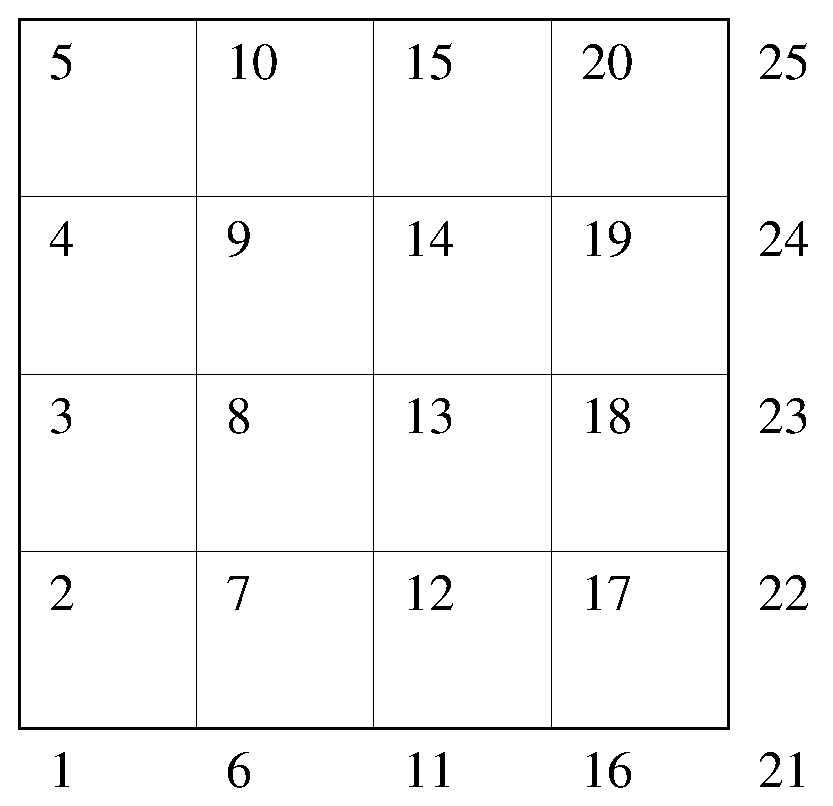
\includegraphics[width=80mm]{FIG/meshglobord.eps}
\caption{Mesh on the original domain. Global ordering.}
\label{figmeshglobord}
\end{center}
\end{figure}

\noindent
{\bf Definition.}
Ordering of nodes or degrees of freedom on particular subdomain which starts from one is called
local \index{local ordering}\index{ordering!local} ordering.

\noindent
The local ordering on particular subdomain looks like the classical ordering of nodes or DOFs on domain.
The local oredring is independent on local orderings on other subdomains. 
Example of the global ordering of nodes is depicted in figure \ref{figmeshlocord}.

\begin{figure}[h]
\begin{center}
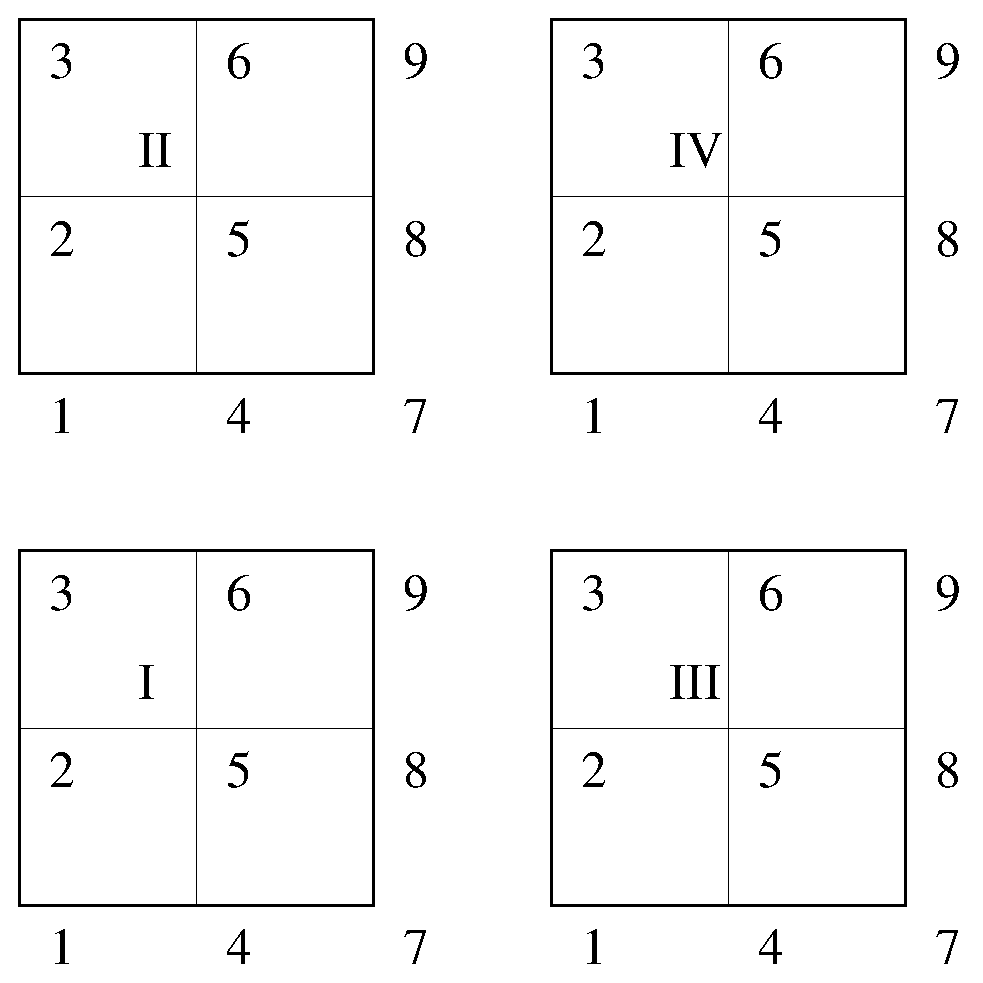
\includegraphics[width=80mm]{FIG/meshlocord.eps}
\caption{Meshes on subdomains obtained by partitioning. Local ordering.}
\label{figmeshlocord}
\end{center}
\end{figure}

\noindent
{\bf Definition.}
Ordering of nodes or degrees of freedom on particular subdomain which is continuous from the first
to the last subdomain is called
global \index{global glued ordering}\index{ordering!global glued} glued ordering.
\label{globgluedorder}

\noindent
The global glued ordering is different from the global ordering because the interface nodes
have at least two different numbers coming from subdomains which share them. The global glued
ordering can be obtained by gluing of local orderings on subdomains where the local numbers
are shifted with respect to the largest number on previous subdomain.
Example of the global glued ordering of nodes is depicted in figure \ref{figmeshglobgluedord}.


\begin{figure}[h]
\begin{center}
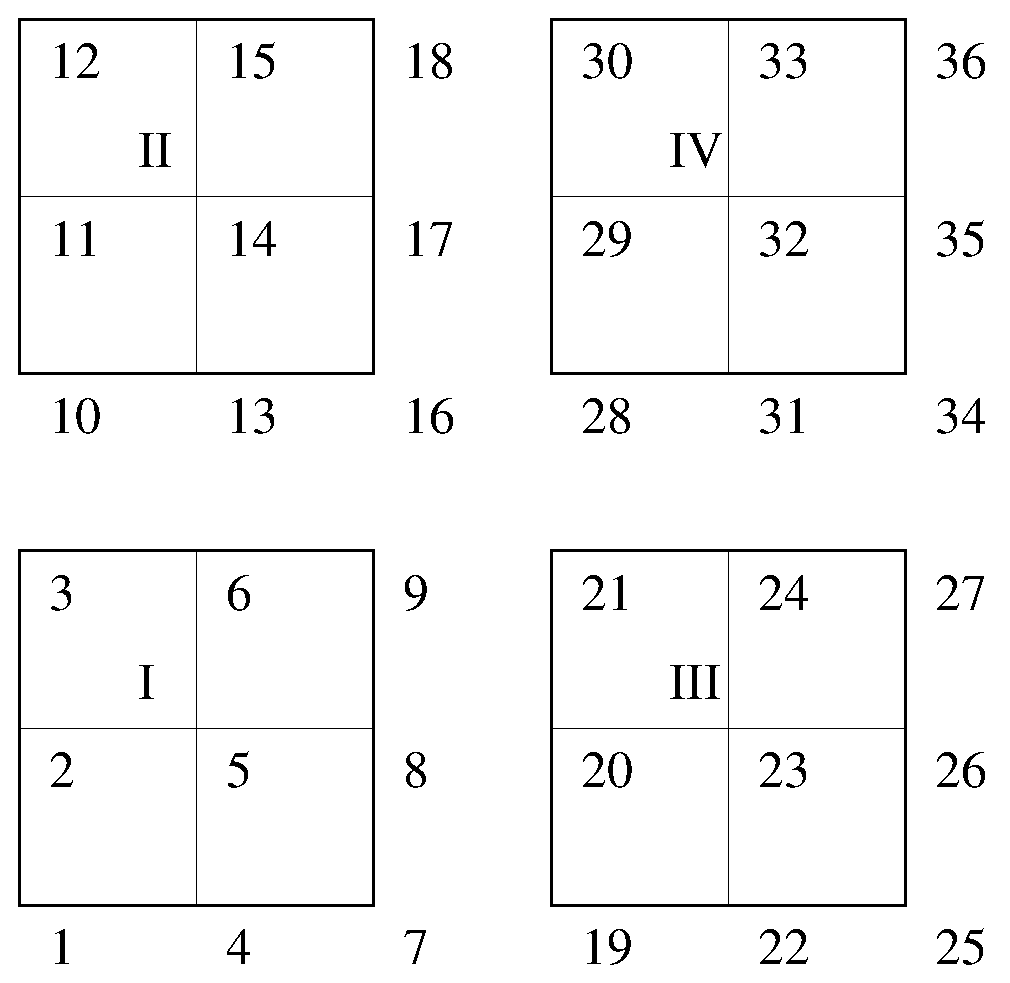
\includegraphics[width=80mm]{FIG/meshglobgluedord.eps}
\caption{Meshes on subdomains obtained by gluing. Global glued ordering.}
\label{figmeshglobgluedord}
\end{center}
\end{figure}

\noindent
{\bf Definition.}
Ordering of nodes or degrees of freedom on the original mesh which covers undecomposed domain is called
negative global \index{negative global ordering}\index{ordering!negative global} ordering if
the interface nodes have their numbers multiplied by minus one.

\noindent
The negative global ordering simplifies searching for the interface nodes and DOFs.
Example of the negative global ordering of nodes is depicted in figure \ref{figmeshnegglobord}.

\begin{figure}[h]
\begin{center}
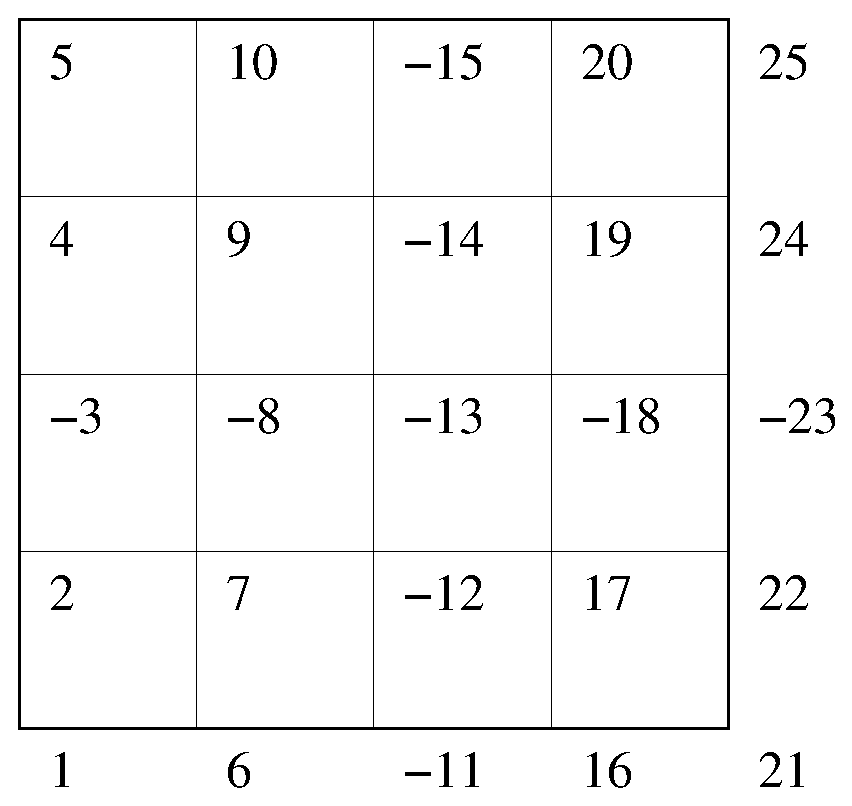
\includegraphics[width=80mm]{FIG/meshnegglobord.eps}
\caption{Mesh on the original domain. Negative global ordering.}
\label{figmeshnegglobord}
\end{center}
\end{figure}

\noindent
{\bf Definition.}
Ordering of interface nodes or degrees of freedom only on the whole problem is called
coarse \index{coarse ordering}\index{ordering!coarse} ordering.

\noindent
The coarse ordering is important in domain decomposition methods beacuse it assures
compatibility among subdomains.
Example of the coarse ordering of nodes is depicted in figure \ref{figmeshcoarseord}.

\begin{figure}[h]
\begin{center}
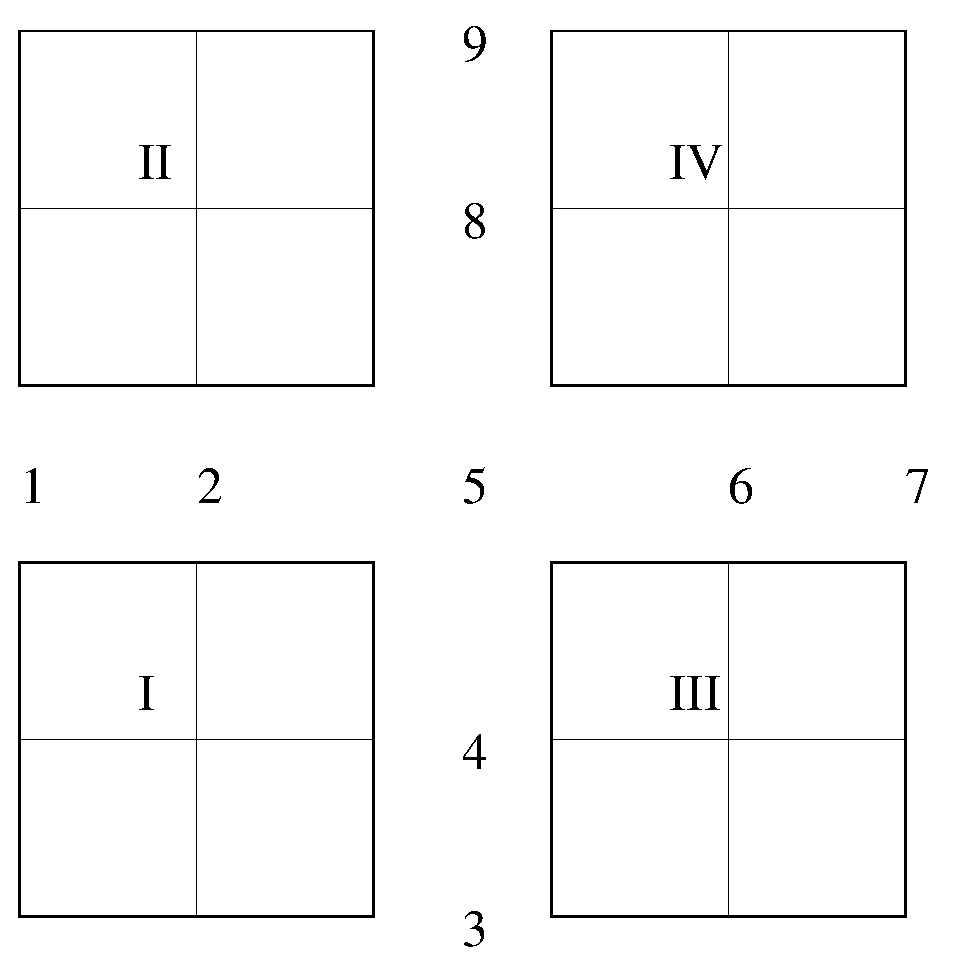
\includegraphics[width=80mm]{FIG/meshcoarseord.eps}
\caption{Coarse ordering.}
\label{figmeshcoarseord}
\end{center}
\end{figure}


Domain decomposition methods contain at least two levels of computation. The local
level deals with subdomains while the coarse level deals with the interface.
Notation coarse follows from the fact, that the interface is similar to a coarse
mesh which can be obtained by elimination of internal nodes or DOFs.
Two orderings of nodes and DOFs are used. The local ordering is used on the local
level and the coarse ordering is used on the coarse level.

The crucial point is correct connection between local and coarse ordering.
The global ordering and the global glued ordering are auxiliary tools for
establishing of the connection between local and coarse ordering.


Connection between local and coarse ordering is created with the help of
\index{\sf ltg}\index{array!{\sf ltg}} array ltg.
Format of the array ltg depends on the variable meshdescription (\ref{sectmeshdescription}).
\index{\sf meshdescription}\index{variable!{\sf meshdescription}}


{\tt
1 2 3 6 7 8 11 12 13
\newline
3 4 5 8 9 10 13 14 15
\newline
11 12 13 16 17 18 21 22 23
\newline
13 14 15 18 19 20 23 24 25
}

{\tt
0 0 1 0 0 2 3 4 5
\newline
1 0 0 2 0 0 5 8 9
\newline
3 4 5 0 0 6 0 0 7
\newline
5 8 9 6 0 0 7 0 0
}


{\tt
1 2 -3 6 7 -8 -11 -12 -13
\newline
-3 4 5 -8 9 10 -13 -14 -15
\newline
-11 -12 -13 16 17 -18 21 22 -23
\newline
-13 -14 -15 -18 19 20 -23 24 25
}


%%%%%%%%%%%%%%%%%%%%%%%%%%%%%%%%%%%%%%%%%%%%%%%%%%%%%%%%
%%%%%%%%%%%%%%%%%%%%%%%%%%%%%%%%%%%%%%%%%%%%%%%%%%%%%%%%
%%%%%%%%%%%%%%%%%%%%%%%%%%%%%%%%%%%%%%%%%%%%%%%%%%%%%%%%
%%%%%%%%%%%%%%%%%%%%%%%%%%%%%%%%%%%%%%%%%%%%%%%%%%%%%%%%
\section{Implementation}

{\bf variant: boundary nodes}

\begin{itemize}
\item
mefel\_init (int argc, char *argv[],stochdriver *stochd) (mefelinit.cpp)

\item
$\Uparrow$ read (XFILE *in) (mechtop.cpp)

\item
$\Uparrow$ Gtm--$>$read\_seq\_top (Mp--$>$ssle--$>$feti.ns,in) --- creates object stop of the class seqtop,

\item
$\Uparrow$ stop--$>$read\_ltg (XFILE *in) (seqtop.cpp) --- allocates and reads array ltg,
local to global correspondence,
ltg[i][j]=k - the j-th node on the i-th subdomain has coarse number k,
k$>$-1 - number of coarse unknown,
k=-1 - the node is internal node,
\newline
$\Uparrow$ stop--$>$read\_nnsd (in); --- allocates and reads array nnsd,
array containing number of nodes on subdomains,
it contains nproc components,
nnsd[i]=j - j nodes are defined on the i-th subdomain,


\item 
gt--$>$stop--$>$compute\_multiplicity (out); 
\newline
array nbnd is allocated, 
array containing list of numbers of boundary/interface nodes on subdomains,
it contains ns components,
nbnd[i]=j - the i-th domain contains j boundary/interface nodes,
\newline
multip is allocated, 
array containing number of subdomains which each boundary/interface node belongs to,
it contains tnnp or tnbn components, it depends on the type of mesh description,
multip[i]=j - the i-th node belongs to j subdomains,
\newline
nodmultip is allocated,
array containing number of subdomains which share the nodes,
it contains ns, nnsd[i] components,
nodmultip[i][j]=k - the j-th node of the i-th subdomain belongs to k subdomains,
\newline
tnbn - total number of interface (boundary) nodes is computed, 


\item
gt--$>$stop--$>$find\_boundary\_nodes (out);
\newline
lgnbn is allocated, 
array containing list of global numbers of interface nodes,
lgnbn[i][j]=k - the j-th interface node on the i-th subdomain has global number k,
\newline
lnbn is allocated,
array containing numbers of boundary nodes,
it contains ns, nbnd[i] components,
lnbn[i][j]=k - the j-th boundary node on the i-th subdomain has local number k,
\newline
nind is allocated,
array containing list of numbers of internal nodes on subdomains,
it contains ns components,
nind[i]=j - the i-th domain contains j internal nodes,
\newline
lnin is allocated,
array containing numbers of internal nodes,
it contains ns, nind[i] components,
lnin[i][j]=k - the j-th internal node on the i-th subdomain has local number k,


\item
gt--$>$stop--$>$rewrite\_ltg (); --- array ltg is rewritten,

\item
object selnodfeti of the class seqselnodes (feti.ns,gt--$>$stop--$>$nnsd,fetinodes,gt--$>$stop--$>$md,out,1); is allocated,
\newline
nsndom is allocated,
numbers of selected nodes,
nsndom[i]=j - there are j selected nodes on the i-th subdomain,
\newline
lsnl is allocated,
list of selected nodes - local numbers,
lsnl[i][j]=k - the j-th selected node on the i-th subdomain has local number k,
lsnl contains ns,nsn[i] components,
\newline
lsng is allocated,
list of selected nodes - global numbers,
lsng[i][j]=k - the j-th selected node on the j-th subdomain has global/coarse number k,
lsng contains ns, nsn[i] components,


\item
selnodfeti--$>$nodes\_on\_master (gt--$>$nn,out);
\newline
gnn is allocated,
group node numbers (see partop.h),
gnn[i][j]=k - the j-th selected node on the i-th subdomain has group number k,
\newline
tnsn - total number of selected nodes is computed,

\item
selnodfeti--$>$node\_multiplicity (out);
\newline
nodmultip is allocated,
node multiplicity,
nodmultip[i]=j - the i-th selected node is shared by j subdomains,
it contains tnsn components,

\item
selnodfeti--$>$number\_all\_dofs (gt,out);
\newline
ndofdom is allocated,
array of numbers of DOFs on subdomains,
it contains prescribed values before code number generation,
after code number generation, only unknown (unconstrained DOFs) are taken into account,
array is rewritten in the function schur\_ordering,
ndofdom[i]=j - the i-th subdomain contains j DOFs,

\item
selnodfeti--$>$ndofn\_on\_master (gt,out);
\newline
ndofnmas is allocated,
array of DOFs at selected nodes,
ndofnmas[i][j]=k - the j-th node on the i-th subdomain contains k DOFs,

\item
selnodfeti--$>$dof\_indicators (gt,out);
\newline
dofmas is allocated,
array of DOFs or indicators on master,
dofmas[i][j][k]=l - the k-th DOF at the j-th selected node on the i-th subdomain has value l,


\item
selnodfeti--$>$group\_local\_nodes (out);
\newline
ljn is allocated,
list of joint nodes to selected nodes assumed as coarse nodes,
ljn[i][j]=k - the j-th node connected to the i-th coarse node has local number k,
ljn contains tnsn rows and nodmultip columns,
\newline
lsn is allocated,
list of subdomain numbers which contain connected nodes to coarse nodes,
lsn[i][j]=k - the j-th node connected to the i-th coarse node belongs to the k-th subdomain,
lsn contains tnsn rows and nodmultip columns,


\item
selnodfeti--$>$dof\_feti (out);
\newline
ndofnsn is allocated,
array of numbers of DOFs for selected nodes,
ndofnsn[i]=j - the i-th selected node (in group ordering) has j DOFs,
it contains tnsn components,
\newline
doffeti is allocated,
code numbers / indicators for FETI method,
doffeti[i][j][k]=l - the k-th DOF on the j-th connected node to the i-th coarse node has code number / indicator l,

\item
selnodfeti--$>$number\_contrib (out);
\newline
ndofdom is allocated,
array of numbers of DOFs on subdomains,
it contains prescribed values before code number generation,
after code number generation, only unknown (unconstrained DOFs) are taken into account,
array is rewritten in the function schur\_ordering,
ndofdom[i]=j - the i-th subdomain contains j DOFs,
\newline
ncndom is allocated,
number of contributing nodes in the FETI method,
ncndom[i]=j - the i-th subdomain contributes to the coarse problem by j nodes,

\item
selnodfeti--$>$contrib\_dofs (gt,out);
\newline
ndofdom
array of numbers of DOFs on subdomains,
it contains prescribed values before code number generation,
after code number generation, only unknown (unconstrained DOFs) are taken into account,
array is rewritten in the function schur\_ordering,
ndofdom[i]=j - the i-th subdomain contains j DOFs,
\newline
ldof
list of code numbers which contribute to the coarse problem,
ldof[i][j]=k - the j-th DOF on the i-th subdomain has local code number k,
\newline
cndom
code numbers on master,
cndom[i][j]=k - the j-th DOF on the i-th subdomain has group code number k,


\item
feti.initiate (selnodfeti,gt,out);
\newline
ncdofd
array of numbers of unknowns (DOFs) contributing to the coarse problem
ncdofd contains nproc components
ncdofd[i]=j - the i-th subdomains contributes to coarse problem by j contributions
\newline
edofs is allocated
array containing code numbers contributing to the coarse problem
extracted values from subdomains to the coarse problem
edofs[i][j]=k - the j-th components contributing to the coarse problem from the i-th subdomains has number k
\newline
ccn
array of coarse code numbers
it contains tnbn rows and ncdofd[i] columns
ccn[i][j]=k - the j-th contribution from the i-th subdomain goes to the k-th coarse unknown

\item
feti.assemble\_subdom\_unknowns (gt,out);
\newline
nsid
node-subdomain correspondence
nsid[i]=j - the i-th node belongs to the j-th subdomain
\newline
ndofdom
numbers of DOFs on subdomains
ndofdom[i]=j - the i-th subdomain contains j DOFs
\newline
cndom
list of DOFs on subdomains
cndom[i][j]=k - the j-th DOF on the i-th subdomain has number k


\end{itemize}

{\bf variant: boundary nodes}
\begin{itemize}
\item
mefel\_init (int argc, char *argv[],stochdriver *stochd) (mefelinit.cpp)

\item
$\Uparrow$ read (XFILE *in) (mechtop.cpp)

\item
$\Uparrow$ Gtm--$>$read\_seq\_top (Mp--$>$ssle--$>$feti.ns,in) --- creates object stop of the class seqtop,

\item
mefel\_init (mefelinit.cpp) $=>$ Mt--$>$read (mechtop.cpp) $=>$ Gtm--$>$read\_seq\_top (gtopology.cpp) $=>$ stop--$>$read\_nnsd (in); (seqtop.cpp) --- allocates and reads array nnsd,
array containing number of nodes on subdomains,
it contains nproc components,
nnsd[i]=j - j nodes are defined on the i-th subdomain,
\newline
$\Uparrow$ stop--$>$read\_ltg (XFILE *in) (seqtop.cpp) --- allocates and reads array ltg,
local to global correspondence,
ltg[i][j]=k - the j-th node on the i-th subdomain has coarse number k,
k$>$-1 - number of coarse unknown,
k=-1 - the node is internal node,

\end{itemize}

%%%%%%%%%%%%%%%%%%%%%%%%%%%%%%%%%%%%%%%%%%%%%%%%%%%%%%%%%%%%%%%%%%%%%%%%
%%%%%%%%%%%%%%%%%%%%%%%%%%%%%%%%%%%%%%%%%%%%%%%%%%%%%%%%%%%%%%%%%%%%%%%%
%%%%%%%%%%%%%%%%%%%%%%%%%%%%%%%%%%%%%%%%%%%%%%%%%%%%%%%%%%%%%%%%%%%%%%%%
%%%%%%%%%%%%%%%%%%%%%%%%%%%%%%%%%%%%%%%%%%%%%%%%%%%%%%%%%%%%%%%%%%%%%%%%
\section{Sequential execution of domain decomposition algorithms}

\begin{itemize}
\item
finite element mesh in the JKTK format has to be prepared, the file with mesh may be
named mesh.aux
\item
input file to METIS decomposer has to be prepared, the code metisprep may be used,
{\tt metisprep mesh.aux mesh.txt}
\item
the mesh has to be decomposed into n submeshes, e.g.
{\tt partdmesh mesh.txt n}, file mesh.txt.epart.n will be created,
\item
one file with all submeshes in the JKTK format has to be generated,
{\tt seqdd mesh.aux mesh.txt.epart.n mesh.top n}, the file mesh.top is in the
JKTK format which is extended at the end by the list of numbers of nodes on 
subdomains and for each subdomain there is list of global node numbers
\end{itemize}

%%%%%%%%%%%%%%%%%%%%%%%%%%%%%%%%%%%%%%%%%%%%%%%%%%%%%%%%%%%%%%%%%%%%%%%%
%%%%%%%%%%%%%%%%%%%%%%%%%%%%%%%%%%%%%%%%%%%%%%%%%%%%%%%%%%%%%%%%%%%%%%%%
%%%%%%%%%%%%%%%%%%%%%%%%%%%%%%%%%%%%%%%%%%%%%%%%%%%%%%%%%%%%%%%%%%%%%%%%
%%%%%%%%%%%%%%%%%%%%%%%%%%%%%%%%%%%%%%%%%%%%%%%%%%%%%%%%%%%%%%%%%%%%%%%%
\section{Automatic Subdomains Detection}

Automatic subdomain detection could be used only for conforming meshes and
twodimensional problems at this time.
Automatic subdomain detection is used e.g. in problems hemivariational inequalities.

It is based on global glued ordering (see \ref{globgluedorder}).

gtopology::auto\_subdom\_detection

\begin{itemize}
\item
gtopology::edges --- function assembles list of adjacent nodes to nodes (adjacnodes),
array of objects gedges of the class gedge are allocated and initiated
\item
gtopology::edgenode\_sorting () --- function sorts first and last nodes on edges
\item
gtopology::prev\_next\_edges --- function searches for previous and next edges for each edge
\item
gtopology::edge\_series () --- function searches for series of edges
\item
gtopology::edge\_elem --- function assignes numbers of element to edges
\item
gtopology::edge\_dirvect () --- function computes direction vectors of edges
\item
gtopology::edge\_normvect () --- function computes direction vectors of edges
\item
gtopology::normvectorient () --- function checkes orientation of normal vectors
\item
gtopology::create\_ltg (FILE *out) --- 
\end{itemize}


%%%%%%%%%%%%%%%%%%%%%%%%%%%%%%%%%%%%%%%%%%%%%%%%%%%%%%%%%%%%%%%%%%%%%%%%
%%%%%%%%%%%%%%%%%%%%%%%%%%%%%%%%%%%%%%%%%%%%%%%%%%%%%%%%%%%%%%%%%%%%%%%%
%%%%%%%%%%%%%%%%%%%%%%%%%%%%%%%%%%%%%%%%%%%%%%%%%%%%%%%%%%%%%%%%%%%%%%%%
%%%%%%%%%%%%%%%%%%%%%%%%%%%%%%%%%%%%%%%%%%%%%%%%%%%%%%%%%%%%%%%%%%%%%%%%
\section{Sequential Schur Complement Method}

nnsd - numbers of nodes on subdomains
9 9 9 9

ltg 

 1  2  3  6  7  8 11 12 13

11 12 13 16 17 18 21 22 23

 3  4  5  8  9 10 13 14 15

13 14 15 18 19 20 23 24 25

tnnp=25

amultip - number of subdomains which each node belongs to
 1 1 2 1 1 1 1 2 1 1 2 2 4 2 2 1 1 2 1 1 1 1 2 1 1

tnbn=9

nbnd  - numbers of boundary/interface nodes on subdomains

5 5 5 5

nind - numbers of internal nodes on subdomains

4 4 4 4

nodmultip - 

 1 1 2 1 1 2 2 2 4

 2 2 4 1 1 2 1 1 2

 2 1 1 2 1 1 4 2 2

 4 2 2 2 1 1 2 1 1


lnbn - local numbers of interface/boundary nodes

 3 6 7 8 9

 1 2 3 6 9

 1 4 7 8 9

 1 2 3 4 7

lnbn - local numbers of internal nodes

 1 2 4 5

 4 5 7 8

 2 3 5 6

 5 6 8 9


ggnbn - global glued numbers of interface/boundary nodes on subdomain


 3 6 7 8 9

10 11 12 15 18

19 22 25 26 27

28 29 30 31 34


ggnin - global glued numbers of internal nodes on subdomain

 1 2 4 5

13 14 16 17

20 21 23 24 

32 33 35 36

icnbn - coarse numbers of interface/boundary nodes on subdomain


 1 2 3 4 5

 3 4 5 8 9

 1 2 5 6 7

 5 6 7 8 9

icmultip - coarse-local correspondence 

 coarse node      0, number of nodes  2

 coarse node      1, number of nodes  2

 coarse node      2, number of nodes  2

 coarse node      3, number of nodes  2

 coarse node      4, number of nodes  4

 coarse node      5, number of nodes  2

 coarse node      6, number of nodes  2

 coarse node      7, number of nodes  2

 coarse node      8, number of nodes  2


ggnbncn - global glued numbers of boundary/interface nodes

 coarse node      0   ggn      3, sub.   1   ggn     19, sub.   3

 coarse node      1   ggn      6, sub.   1   ggn     22, sub.   3

 coarse node      2   ggn      7, sub.   1   ggn     10, sub.   2

 coarse node      3   ggn      8, sub.   1   ggn     11, sub.   2

 coarse node      4   ggn      9, sub.   1   ggn     12, sub.   2   ggn     25, sub.   3   ggn     28, sub.   4

 coarse node      5   ggn     26, sub.   3   ggn     29, sub.   4

 coarse node      6   ggn     27, sub.   3   ggn     30, sub.   4

 coarse node      7   ggn     15, sub.   2   ggn     31, sub.   4

 coarse node      8   ggn     18, sub.   2   ggn     34, sub.   4


nsndom - numbers of slected nodes on subdomains
5 5 5 5

ggnsn - global glued numbers of selected nodes

  3  6  7  8  9

 10 11 12 15 18

 19 22 25 26 27

 28 29 30 31 34

snndofdom - numbers of DOFs on subdomains

10 10 10 10

snndofnmas - numbers of DOFs on selected nodes

2 2 2 2 2

2 2 2 2 2

2 2 2 2 2

2 2 2 2 2

sndofmas - DOFs indicators on master

  0  0
  1  0
  1  0
  1  0
  1  0

  1  0
  1  0
  1  0
  1  0
  1  0

  0  0
  1  0
  1  0
  1  0
  1  0

  1  0
  1  0
  1  0
  1  0
  1  0

tndofsn=8

cndom - code numbers of Schur ordering

1 2 3 4

2 3 4 7 8

1 4 5 6

4 5 6 7 8

ndofdom - number of DOFs on subdomains 
6 9 6 9

cndom - array of code numbers of DOFs on subdomains 

 1 2 13 14 15 16

 3 4 5 6 17 18 19 20 21

 7 8 22 23 24 25

 9 10 11 12 26 27 28 29 30


adr in skyline

 0 1 3 5 9 14 19

 0 1 3 6 10 15 21 27 34 42

 0 1 3 6 10 15 21

 0 1 3 6 10 15 21 28 36 45


%%%%%%%%%%%%%%%%%%%%%%%%%%%%%%%%%%%%%%%%%%%%%%%%%%%%%%%%%%%%%%%%%%%%%%%%
%%%%%%%%%%%%%%%%%%%%%%%%%%%%%%%%%%%%%%%%%%%%%%%%%%%%%%%%%%%%%%%%%%%%%%%%
%%%%%%%%%%%%%%%%%%%%%%%%%%%%%%%%%%%%%%%%%%%%%%%%%%%%%%%%%%%%%%%%%%%%%%%%
%%%%%%%%%%%%%%%%%%%%%%%%%%%%%%%%%%%%%%%%%%%%%%%%%%%%%%%%%%%%%%%%%%%%%%%%
\section{Sequential FETI Method}
12. 7. 2012

Mp--$>$ssle--$>$prepare\_data (Ndofm,Gtm,Out); in mefelinit.cpp

\hspace{10mm} top--$>$stop--$>$coarse\_local\_map (top,out);

\hspace{20mm}  seqtop::compute\_multiplicity (top,out);

\hspace{30mm}  seqtop::assemble\_multip (out);

\hspace{30mm}  seqtop::coupled\_dofs (top,out);

\hspace{30mm}  seqtop::assemble\_nbnd\_nind (out);

\hspace{30mm}  seqtop::assemble\_nodmultip (out);

\hspace{30mm}  seqtop::assemble\_dofind (top,out);

\hspace{20mm}  seqtop::node\_local\_numbers (out);

\hspace{20mm}  seqtop::node\_global\_glued\_numbers (out);

\hspace{20mm}  seqtop::node\_coarse\_numbers (out);

\hspace{20mm}  seqtop::node\_coarse\_global\_glued\_map (out);

\hspace{20mm}  seqtop::node\_coarse\_local\_map (out);

\hspace{10mm}  ndof[0]=selnodfeti--$>$prepare\_feti (feti.fetiimpl,top,out);

\hspace{20mm}  seqselnodes::define\_feti\_implementation (fi);

\hspace{20mm}  seqselnodes::node\_coarse\_numbers (out);

\hspace{20mm}  seqselnodes::number\_contrib\_dofs (top,out);

\hspace{20mm}  seqselnodes::dof\_feti (top,out);

\hspace{20mm}  seqselnodes::top--$>$cngen=1;

\hspace{20mm}  seqselnodes::ndof = top--$>$codenum\_generation (out);

\hspace{20mm}  seqselnodes::contrib\_dofs\_ln (top,out);

\hspace{20mm}  seqselnodes::contrib\_dofs\_cn (out);

\hspace{10mm}   feti.initiate (selnodfeti,top,out);

\hspace{10mm} feti.assemble\_subdom\_unknowns (top,out);

\noindent
{\color{red} void seqtop::assemble\_multip (FILE *out)}
the function assembles the array {\sf bmultip} or {\sf amultip},
the function computes the variables {\sf tnnp} or {\sf tnbn}.

\noindent
{\color{red} void seqtop::coupled\_dofs (gtopology *top,FILE *out)}
the function searches for coupled DOFs which are shared by interfaces
the number of coupled DOFs on interfaces {\sf ncdof} is determined
if {\sf ncdof}$>0$, arrays {\sf coupdofmas} and {\sf coupdof}
are allocated and assmebled

\noindent
{\color{red} void seqtop::update\_multip (gtopology *top,FILE *out)}
the function updates node multiplicity,
the attributes the total number of boundary nodes {\sf tnbn} and
the total number of nodes in problem (if possible, this number cannot be
obtained in the case of md=bound\_nodes) {\sf tnnp},
array {\sf amultip} array of all node multiplicity, it is assembled if md=all\_nodes
array {\sf bmultip} array of interface/boundary node multiplicity, it is assembled if md=bound\_nodes
array {\sf nodmultip} array of node multiplicity (on all subdomains)

\noindent
{\color{red} void seqtop::assemble\_nbnd\_nind (FILE *out)}
the function assembles the arrays {\sf nbnd} and {\sf nind}

\noindent
{\color{red} void seqtop::assemble\_nodmultip (FILE *out)}
the function assembless the array {\sf nodmultip}

\noindent
{\color{red} void seqtop::assemble\_dofind (gtopology *top,FILE *out)}
the function assembless the array {\sf dofind} if it has not been assembled yet


\noindent
{\color{red} void seqtop::node\_local\_numbers (FILE *out)}
the function assembles local numbers of nodes
{\sf lnbn} - local numbers of interface/boundary nodes
{\sf lnin} - local numbers of internal nodes

\noindent
{\color{red} void seqtop::node\_global\_glued\_numbers (FILE *out)}
the function assembles global glued numbers of nodes
{\sf ggnbn} - global glued numbers of interface/boundary nodes
{\sf ggnin} - global glued numbers of internal nodes

\noindent
{\color{red} void seqtop::node\_coarse\_numbers (FILE *out)}
the function assembles coarse numbers of nodes
{\sf icnbnmas} - coarse numbers of interface/boundary nodes
{\sf icmultip} - number of multiplicity of boundary/interface nodes

\noindent
{\color{red} void seqtop::node\_coarse\_global\_glued\_map (FILE *out)}
the function assembles coarse - global glued numbers map
{\sf ggnbncn} - global glued numbers of boundary/interface nodes of the coarse node
{\sf sid} - subdomain id of interface/boundary nodes of the coarse node

\noindent
{\color{red} void seqtop::node\_coarse\_local\_map (FILE *out)}
the function assembles coarse - local numbers map
{\sf lnbncn} - local numbers of boundary/interface nodes of the coarse node
{\sf sid} - subdomain id of interface/boundary nodes of the coarse node













\section{List of attributes}
\begin{itemize}
\item
{\sf amultip (long *amultip;)} array containing number of subdomains which each node belongs to,
it contains {\sf tnnp} components,
{\sf amultip[i]=j} - the i-th node belongs to j subdomains,
the array is assembled in the function {\sf assemble\_multip (FILE *out)}

\item
{\sf bmultip (long *bmultip;)} array containing number of subdomains which each boundary/interface node belongs to, it contains {\sf tnbn} components,
{\sf bmultip[i]=j} - the i-th interface/boundary node belongs to j subdomains,
the array is assembled in the function {\sf assemble\_multip (FILE *out)}

\item
{\sf coupdof (long **coupdof;)} the array containing indicators of coupled DOFs,
it has {\sf ns, ncdof} components,
{\sf coupdof[i][j]=k} - the j-th coupled DOFs on the i-th subdomain is shared by k nodes,
array is allocated in the function {\sf coupled\_dofs}

\item
{\sf coupdofmas (long *coupdofmas;)} array containing suspicious indicators of coupled DOFs,
it has {\sf ncdof} components,
{\sf coupdofmas[i]=0} - the i-th coupled DOF is not a boundary/interface DOF,
{\sf coupdofmas[i]=1} - the i-th coupled DOF is a boundary/interface DOF,
array is allocated in the function {\sf coupled\_dofs}

\item
{\sf dofind (long **dofind;)} array containing DOF indicators,
if there are coupled DOFs, it is not enough to deal with nodes,
DOFs have to be split to internal and boundary/interface,
it has {\sf nn, ndofn[i]} components ({\sf nn} is the total number of nodes)
{\sf dofind[i][j]=0} - the j-th DOF in the i-th node is internal,
{\sf dofind[i][j]=1} - the j-th DOF in the i-th node is boundary/interface,
the array is allocated in the function {\sf update\_multiplicity}


\item
{\sf ggnbn (long **ggnbn;)} array containing global glued numbers of boundary/interface nodes,
it contains {\sf ns, nbnd[i]} components,
{\sf ggnbn[i][j]=k} - the j-th boundary/interface node on the i-th subdomain has global glued number k
array is allocated in the function {\sf node\_global\_glued\_numbers}

\item
{\sf ggnbncn (long **ggnbncn;)} global glued numbers of boundary/interface nodes appropriate to coarse node,
it contains global glued numbers of boundary/interafce nodes of each coarse node
it contains {\sf tnbn} rows and {\sf icmultip[i]} columns,
{\sf ggnbncn[i][j]=k} - the j-th node shared by the i-th coarse node has global glued number k,
aray is allocated in the function {\sf node\_coarse\_global\_glued\_map}
  
\item
{\sf ggnin (long **ggnin;)} array containing global glued numbers of internal nodes,
it contains {\sf ns, nind[i]} components,
{\sf ggnin[i][j]=k} - the j-th internal node on the i-th subdomain has global glued number k,
array is allocated in the function {\sf node\_global\_glued\_numbers}

\item
{\sf icnbnmas (long **icnbnmas;)} array containing coarse numbers of interface/boundary nodes,
it contains {\sf ns, nbnd[i]} components,
{\sf icnbnmas[i][j]=k} - the j-th boundary node on the i-th subdomain has coarse number k,
the array is allocated in the function {\sf node\_coarse\_numbers}

\item
{\sf icmultip (long *icmultip;)} array containing node multiplicity of boundary/interface nodes,
it contains {\sf tnbn} components,
{\sf icmultip[i]=j} - the i-th boundary/interface node belongs to j subdomains,
array is allocated in the function {\sf node\_coarse\_numbers}

\item
{\sf lnbn (long **lnbn;)} array containing local numbers of interface/boundary nodes
it contains {\sf ns, nbnd[i]} components,
{\sf lnbn[i][j]=k} - the j-th boundary node on the i-th subdomain has local number k,
the array is allocated in the function {\sf node\_local\_numbers}

\item
{\sf lnin (long **lnin;)} array containing local numbers of internal nodes,
it contains {\sf ns, nind[i]} components,
{\sf lnin[i][j]=k} - the j-th internal node on the i-th subdomain has local number k,
array is allocated in the function {\sf node\_local\_numbers}

\item
{\sf ncdof (long ncdof;)} the number of coupled DOFs,
it is determined in the function {\sf coupled\_dofs}

\item
{\sf nodmultip (long **nodmultip;)} array containing number of subdomains which share the nodes,
it contains {\sf ns, nnsd[i]} components,
{\sf nodmultip[i][j]=k} - the j-th node of the i-th subdomain belongs to k subdomains
the array is assembled in the function {\sf update\_multip (gtopology *top,FILE *out)}
or {\sf assemble\_nodmultip (FILE *out)}.
 
\item
{\sf (long **sid;)} subdomain id of interface/boundary nodes appropriate to coarse node,
it contains {\sf tnbn} rows and {\sf icmultip[i]} columns,
{\sf sid[i][j]=k} - the j-th node shared by the i-th coarse node belongs to the k-th subdomain,
array is allocated in the function {\sf node\_coarse\_local\_map} or {\sf node\_coarse\_global\_glued\_map}

\item
{\sf tnbn (long tnbn;)} the total number of interface (boundary) nodes,
this number is determined in the function {\sf compute\_multiplicity}

\item
{\sf tnnp (long tnnp;)} the total number of nodes in the whole problem,
this number cannot be obtained in the case of mesh description = bound\_nodes
this number is determined in the function {\sf compute\_multiplicity}
\end{itemize}


%%%%%%%%%%%%%%%%%%%%%%%%%%%%%%%%%%%%%%%%%%%%%%%%%%%%%%%%%%%%%%%%%%%%%%%%
%%%%%%%%%%%%%%%%%%%%%%%%%%%%%%%%%%%%%%%%%%%%%%%%%%%%%%%%%%%%%%%%%%%%%%%%
%%%%%%%%%%%%%%%%%%%%%%%%%%%%%%%%%%%%%%%%%%%%%%%%%%%%%%%%%%%%%%%%%%%%%%%%
%%%%%%%%%%%%%%%%%%%%%%%%%%%%%%%%%%%%%%%%%%%%%%%%%%%%%%%%%%%%%%%%%%%%%%%%
\section{Sequential FETI Method}

1 \# mesh description - this is boundary nodes description

4 \# the number of subdomains

9 9 9 9

 1  2  3  6  7  8 11 12 13

 3  4  5  8  9 10 13 14 15

11 12 13 16 17 18 21 22 23

13 14 15 18 19 20 23 24 25


tnnp - total number of nodes in whole problem is 25


 node      0  amultip   1

 node      1  amultip   1

 node      2  amultip   2

 node      3  amultip   1

 node      4  amultip   1

 node      5  amultip   1

 node      6  amultip   1

 node      7  amultip   2

 node      8  amultip   1

 node      9  amultip   1

 node     10  amultip   2

 node     11  amultip   2

 node     12  amultip   4

 node     13  amultip   2

 node     14  amultip   2

 node     15  amultip   1

 node     16  amultip   1

 node     17  amultip   2

 node     18  amultip   1

 node     19  amultip   1

 node     20  amultip   1

 node     21  amultip   1

 node     22  amultip   2

 node     23  amultip   1

 node     24  amultip   1


 ncdof - the number of coupled DOFs 0


 total number of boundary nodes in whole problem is 9



 numbers of interface/boundary nodes on each subdomain 


 5 5 5 5


 numbers of internal nodes on each subdomain 

 4 4 4 4


 Multiplicity of nodes on subdomain

 1 1 2 1 1 2 2 2 4

 2 1 1 2 1 1 4 2 2

 2 2 4 1 1 2 1 1 2

 4 2 2 2 1 1 2 1 1



 local numbers of interface/boundary nodes on subdomain (lnbn)

 3 6 7 8 9

 1 4 7 8 9

 1 2 3 6 9

 1 2 3 4 7


 local numbers of internal nodes on subdomain (lnin)

 1 2 4 5

 2 3 5 6

 4 5 7 8

 5 6 8 9


 global glued numbers of interface/boundary nodes on subdomain (ggnbn)

 domain 0
 3 6 7 8 9

 10 13 16 17 18

 19 20 21 24 27

 28 29 30 31 34


 global glued numbers of internal nodes on subdomain (ggnin)

 1 2 4 5

 11 12 14 15

 22 23 25 26

 32 33 35 36


 coarse numbers of interface/boundary nodes on subdomain (icnbnmas)

 domain 0
      0        1
      1        2
      2        3
      3        4
      4        5

 domain 1
      0        1
      1        2
      2        5
      3        6
      4        7

 domain 2
      0        3
      1        4
      2        5
      3        8
      4        9

 domain 3
      0        5
      1        6
      2        7
      3        8
      4        9


 coarse-local correspondence (icmultip)

 coarse node      0, number of nodes  2
 coarse node      1, number of nodes  2
 coarse node      2, number of nodes  2
 coarse node      3, number of nodes  2
 coarse node      4, number of nodes  4
 coarse node      5, number of nodes  2
 coarse node      6, number of nodes  2
 coarse node      7, number of nodes  2
 coarse node      8, number of nodes  2


 coarse-global glued correspondence 

 coarse node      0, number of nodes  2   node 0, global glued number      3, subdomain id    1   node 1, global glued number     10, subdomain id    2
 coarse node      1, number of nodes  2   node 0, global glued number      6, subdomain id    1   node 1, global glued number     13, subdomain id    2
 coarse node      2, number of nodes  2   node 0, global glued number      7, subdomain id    1   node 1, global glued number     19, subdomain id    3
 coarse node      3, number of nodes  2   node 0, global glued number      8, subdomain id    1   node 1, global glued number     20, subdomain id    3
 coarse node      4, number of nodes  4   node 0, global glued number      9, subdomain id    1   node 1, global glued number     16, subdomain id    2   node 2, global glued number     21, subdomain id    3   node 3, global glued number     28, subdomain id    4
 coarse node      5, number of nodes  2   node 0, global glued number     17, subdomain id    2   node 1, global glued number     29, subdomain id    4
 coarse node      6, number of nodes  2   node 0, global glued number     18, subdomain id    2   node 1, global glued number     30, subdomain id    4
 coarse node      7, number of nodes  2   node 0, global glued number     24, subdomain id    3   node 1, global glued number     31, subdomain id    4
 coarse node      8, number of nodes  2   node 0, global glued number     27, subdomain id    3   node 1, global glued number     34, subdomain id    4


 coarse-global glued correspondence 

 coarse node      0   ggn      3, sub.   1   ggn     10, sub.   2
 coarse node      1   ggn      6, sub.   1   ggn     13, sub.   2
 coarse node      2   ggn      7, sub.   1   ggn     19, sub.   3
 coarse node      3   ggn      8, sub.   1   ggn     20, sub.   3
 coarse node      4   ggn      9, sub.   1   ggn     16, sub.   2   ggn     21, sub.   3   ggn     28, sub.   4
 coarse node      5   ggn     17, sub.   2   ggn     29, sub.   4
 coarse node      6   ggn     18, sub.   2   ggn     30, sub.   4
 coarse node      7   ggn     24, sub.   3   ggn     31, sub.   4
 coarse node      8   ggn     27, sub.   3   ggn     34, sub.   4


 coarse-local correspondence 

 coarse node      0, number of nodes  2   node 0, local number      3, subdomain id    1   node 1, local number      1, subdomain id    2
 coarse node      1, number of nodes  2   node 0, local number      6, subdomain id    1   node 1, local number      4, subdomain id    2
 coarse node      2, number of nodes  2   node 0, local number      7, subdomain id    1   node 1, local number      1, subdomain id    3
 coarse node      3, number of nodes  2   node 0, local number      8, subdomain id    1   node 1, local number      2, subdomain id    3
 coarse node      4, number of nodes  4   node 0, local number      9, subdomain id    1   node 1, local number      7, subdomain id    2   node 2, local number      3, subdomain id    3   node 3, local number      1, subdomain id    4
 coarse node      5, number of nodes  2   node 0, local number      8, subdomain id    2   node 1, local number      2, subdomain id    4
 coarse node      6, number of nodes  2   node 0, local number      9, subdomain id    2   node 1, local number      3, subdomain id    4
 coarse node      7, number of nodes  2   node 0, local number      6, subdomain id    3   node 1, local number      4, subdomain id    4
 coarse node      8, number of nodes  2   node 0, local number      9, subdomain id    3   node 1, local number      7, subdomain id    4


 coarse-local correspondence 

 coarse node      0    loc.n.      3, sub.    1    loc.n.      1, sub.    2
 coarse node      1    loc.n.      6, sub.    1    loc.n.      4, sub.    2
 coarse node      2    loc.n.      7, sub.    1    loc.n.      1, sub.    3
 coarse node      3    loc.n.      8, sub.    1    loc.n.      2, sub.    3
 coarse node      4    loc.n.      9, sub.    1    loc.n.      7, sub.    2    loc.n.      3, sub.    3    loc.n.      1, sub.    4
 coarse node      5    loc.n.      8, sub.    2    loc.n.      2, sub.    4
 coarse node      6    loc.n.      9, sub.    2    loc.n.      3, sub.    4
 coarse node      7    loc.n.      6, sub.    3    loc.n.      4, sub.    4
 coarse node      8    loc.n.      9, sub.    3    loc.n.      7, sub.    4


 list of global glued numbers of selected nodes (ggnsn)

 subdomain    0,  number of selected nodes is nsnmas 5
 global glued node number      3
 global glued node number      6
 global glued node number      7
 global glued node number      8
 global glued node number      9
 subdomain    1,  number of selected nodes is nsnmas 5
 global glued node number     10
 global glued node number     13
 global glued node number     16
 global glued node number     17
 global glued node number     18
 subdomain    2,  number of selected nodes is nsnmas 5
 global glued node number     19
 global glued node number     20
 global glued node number     21
 global glued node number     24
 global glued node number     27
 subdomain    3,  number of selected nodes is nsnmas 5
 global glued node number     28
 global glued node number     29
 global glued node number     30
 global glued node number     31
 global glued node number     34


 total number of selected nodes (tnsn)  9


 local numbers of boundary/interface nodes appropriate to selected coarse node (snlnbncn)

 global glued numbers of boundary/interface nodes appropriate to selected coarse node (snggnbncn)

 subdomain id of interface/boundary nodes appropriate to coarse node (snsid)

 sel. n.      0   snicmultip       2
         2       2       0
         0       9       1

 sel. n.      1   snicmultip       2
         5       5       0
         3      12       1

 sel. n.      2   snicmultip       2
         6       6       0
         0      18       2

 sel. n.      3   snicmultip       2
         7       7       0
         1      19       2

 sel. n.      4   snicmultip       4
         8       8       0
         6      15       1
         2      20       2
         0      27       3

 sel. n.      5   snicmultip       2
         7      16       1
         1      28       3

 sel. n.      6   snicmultip       2
         8      17       1
         2      29       3

 sel. n.      7   snicmultip       2
         5      23       2
         3      30       3

 sel. n.      8   snicmultip       2
         8      26       2
         6      33       3


 numbers of contributing DOFs on subdomains (snndofmas)

 subdomain number      1   14
 subdomain number      2   10
 subdomain number      3   10
 subdomain number      4   10

 total number of DOFs in selected nodes (tndofsn)  20

 code numbers for FETI method (doffeti)


 coarse node      1
         0     0        0     0
         0     0        0     0

 coarse node      2
         0     0        1     2
         1     2        0     0

 coarse node      3
         0     0        3     4
         3     4        0     0

 coarse node      4
         0     0        5     6
         5     6        0     0

 coarse node      5
         0     0        7     8        9    10       11    12
         7     8        0     0        0     0        0     0
         9    10        0     0        0     0        0     0
        11    12        0     0        0     0        0     0

 coarse node      6
         0     0       13    14
        13    14        0     0

 coarse node      7
         0     0       15    16
        15    16        0     0

 coarse node      8
         0     0       17    18
        17    18        0     0

 coarse node      9
         0     0       19    20
        19    20        0     0


 array of numbers of DOFs on subdomains at selected nodes (snndofmas)


 list of code numbers which contribute to the coarse problem (lndofmas)
 subdomain      0   snndofmas     12
   -5   -6   -7   -8   -9   -10   -11   -12   -11   -12   -11   -12
 subdomain      1   snndofmas      8
   13   14   19   20   -21   -22   -23   -24
 subdomain      2   snndofmas     10
   25   26   27   28   29   30   -35   -36   -41   -42
 subdomain      3   snndofmas     10
   43   44   45   46   47   48   49   50   55   56

 coarse code numbers on master (cndofmas)

 subdomain number      0 (number of DOFs 12)
      0   1
      1   2
      2   3
      3   4
      4   5
      5   6
      6   7
      7   8
      8   9
      9   10
     10   11
     11   12
 subdomain number      1 (number of DOFs 8)
      0   1
      1   2
      2   7
      3   8
      4   13
      5   14
      6   15
      7   16
 subdomain number      2 (number of DOFs 10)
      0   3
      1   4
      2   5
      3   6
      4   9
      5   10
      6   17
      7   18
      8   19
      9   20
 subdomain number      3 (number of DOFs 10)
      0   11
      1   12
      2   13
      3   14
      4   15
      5   16
      6   17
      7   18
      8   19
      9   20


 check of the array edofs 

 domain 0
 edofs       0      -5
 edofs       1      -6
 edofs       2      -7
 edofs       3      -8
 edofs       4      -9
 edofs       5     -10
 edofs       6     -11
 edofs       7     -12
 edofs       8     -11
 edofs       9     -12
 edofs      10     -11
 edofs      11     -12
 domain 1
 edofs       0       1
 edofs       1       2
 edofs       2       7
 edofs       3       8
 edofs       4      -9
 edofs       5     -10
 edofs       6     -11
 edofs       7     -12
 domain 2
 edofs       0       1
 edofs       1       2
 edofs       2       3
 edofs       3       4
 edofs       4       5
 edofs       5       6
 edofs       6     -11
 edofs       7     -12
 edofs       8     -17
 edofs       9     -18
 domain 3
 edofs       0       1
 edofs       1       2
 edofs       2       3
 edofs       3       4
 edofs       4       5
 edofs       5       6
 edofs       6       7
 edofs       7       8
 edofs       8      13
 edofs       9      14

 kontrola pole ndofmas
 ndofmas      0       12
 ndofmas      1       12
 ndofmas      2       18
 ndofmas      3       18

 kontrola pole cndom
 domain 0
 dom      0  dof      0        1
 dom      0  dof      1        2
 dom      0  dof      2        3
 dom      0  dof      3        4
 dom      0  dof      4        5
 dom      0  dof      5        6
 dom      0  dof      6        7
 dom      0  dof      7        8
 dom      0  dof      8        9
 dom      0  dof      9       10
 dom      0  dof     10       11
 dom      0  dof     11       12
 domain 1
 dom      1  dof      0       13
 dom      1  dof      1       14
 dom      1  dof      2       15
 dom      1  dof      3       16
 dom      1  dof      4       17
 dom      1  dof      5       18
 dom      1  dof      6       19
 dom      1  dof      7       20
 dom      1  dof      8       21
 dom      1  dof      9       22
 dom      1  dof     10       23
 dom      1  dof     11       24
 domain 2
 dom      2  dof      0       25
 dom      2  dof      1       26
 dom      2  dof      2       27
 dom      2  dof      3       28
 dom      2  dof      4       29
 dom      2  dof      5       30
 dom      2  dof      6       31
 dom      2  dof      7       32
 dom      2  dof      8       33
 dom      2  dof      9       34
 dom      2  dof     10       35
 dom      2  dof     11       36
 dom      2  dof     12       37
 dom      2  dof     13       38
 dom      2  dof     14       39
 dom      2  dof     15       40
 dom      2  dof     16       41
 dom      2  dof     17       42
 domain 3
 dom      3  dof      0       43
 dom      3  dof      1       44
 dom      3  dof      2       45
 dom      3  dof      3       46
 dom      3  dof      4       47
 dom      3  dof      5       48
 dom      3  dof      6       49
 dom      3  dof      7       50
 dom      3  dof      8       51
 dom      3  dof      9       52
 dom      3  dof     10       53
 dom      3  dof     11       54
 dom      3  dof     12       55
 dom      3  dof     13       56
 dom      3  dof     14       57
 dom      3  dof     15       58
 dom      3  dof     16       59
 dom      3  dof     17       60

\chapter{Changing domains}

In some cases, a problem is defined on a domain which is developping
in time or during analysis. Casting of concrete structure can serve as
a typical example.

In order to describe domain which is developping, additional tools for
nodes and elements have to be defined. Namely, degrees of freedom
and elements have their time function which indicates whether they
are switched on or off. Usually, the time functions have two values,
where 0 means that the entity is switched off and the value 1 means
that the entity is switched on. In more complicated cases, where
several degrees of freedom are connected, the time function has to return
integer number greater than 1. All degrees of freedom with the same
integer number greater than 1 will have the same code number and they
are assumed to be switched on.

Time functions for degrees of freedom are read as constraints.
It means, that the number of constraints must be equal to the
number of all nodes and the following numbers are not stored in
array cn but in array tgf. The array cn is filled by 1 everywhere.
Time functions for elements are read after code numbers on elements
and before the number of materials. They are stored in variable tgf.


%\input{hangingnodes.tex}
%\input{timecontr.tex}
%%%%%%%%%%%%%%%%%%%%%%%%%%%%%%%%%%%%%%%%%%%%%%%%%%%%%%%%%%
%%%%%%%%%%%%%%%%%%%%%%%%%%%%%%%%%%%%%%%%%%%%%%%%%%%%%%%%%%
%%%%%%%%%%%%%%%%%%%%%%%%%%%%%%%%%%%%%%%%%%%%%%%%%%%%%%%%%%
%%%%%%%%%%%%%%%%%%%%%%%%%%%%%%%%%%%%%%%%%%%%%%%%%%%%%%%%%%
\printindex
\end{document}
